\section{Mračná bodov a ich spracovanie}
\noindent Mračno bodov je kolekcia bodov v 3D priestore, kde každý bod je reprezentovaný pomocou XYZ súradníc, okrem ktorých môže obsahovať doplňujúcu informáciu o ich farbe, intenzite a v prípade potreby, aj ďalších špecifických atribútoch. Spájaním veľkého množstva týchto bodov, do jedného súboru zo spoločným súradnicovým systémom, je možné zachytiť úplnú geometriu akéhokoľvek 3D objektu. Vďaka schopnosti poskytovať priestorové súradnice povrchov objektov sa mračná bodov stali preferovaným typom dát pre 3D vizualizácia rôznorodých prostredí. Mračna bodov sa osvedčili, ako jedny z najvhodnejších zdrojov údajov, najmä pri mapovaní rozsiahlych mestských prostredí, pretože získané 3D body obsahujú priame priestorové súradnice geometrických povrchov, čo výrazne zjednodušuje procesy modelovania povrchov a geometrickej rekonštrukcie. \cite{voxel_grid} 
\newline\begin{figure}[!htbp]
  \centering
  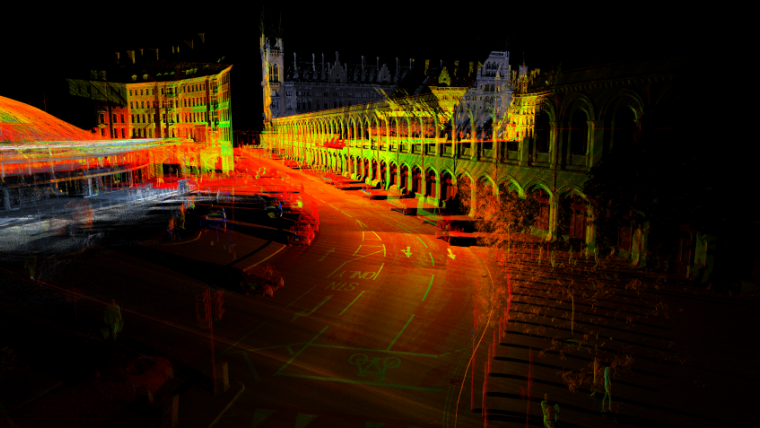
\includegraphics[width=16cm]{img/ukazka_pc.png}
  \caption{Ukážka mračna bodov}
  \label{vzhladobr}
\end{figure}	
\newline\indent Mračna bodov ďalej často nachádzajú využitie v rôznych oblastiach, ako je počítačové videnie, modelovanie terénu, robotika či v rámci medicíny. Spôsoby získavania mračna bodov zahŕňajú rôzne metódy a techniky, pričom každá ponúka jedinečné výhody. Medzi najpopulárnejšie prístupy v oblasti robotiky a priemyslu patrí využitie \acrshort{lidar}-u, stereo kamery a hĺbkovej kamery.

\subsection{Dátové štruktúry pre spracovanie mračna bodov}
\noindent Neupravené mračná bodov sú obvykle neštruktúrované, majú nerovnomernú hustotu bodov a navyše, ich kvalita môže byť odlišná v rôznych častiach, čo býva považované za nevhodné pre ich adekvátnu použiteľnosť. Okrem toho pri mračnách bodov získaných z viacerých zdrojov je zvyčajne veľké množstvo prekrývajúcich bodov, čo zbytočne zvyšuje pamäťové a výpočtové nároky. \cite{voxel_grid} \cite{struktury} \newline\indent Pri mnohých algoritmoch je kritické získať informácie o susedných bodoch, avšak v prípade veľkých a neštruktúrovaných mračien je táto úloha časovo a výpočtovo náročná. Preto pre tento účel existujú dátové štruktúry, ktoré umožňujú organizáciu mračna bodov do efektívnejších usporiadaní.

\subsubsection{Voxelová mriežka}
\noindent Voxelová mriežka (z ang. Voxel grid) je zložená z voxelov, ktoré sa dajú charakterizovať, ako elementárne bloky 3D priestoru. Môžeme si ich predstaviť, ako 3D analógiu pixelov. Majú síce tvar kvádrov so stenami, rohmi a hranami, ale dátovo nie sú nikdy uložené ako celé kvádre. Namiesto toho sa vo voxelovej reprezentácií používa buď stredný bod alebo rohové body (t.j. vrcholy) kvádra pre jeho celú reprezentáciu. Keď sa dva voxely dotýkajú stenou, rohom alebo hranou, sú považované za susedné. Celé mračno bodov je takto rozdelené na osobitné voxely, pričom body vo vnútri daného voxelu sú reprezentované týmto voxelom a zároveň daný voxel je reprezentovaný týmito bodmi. To znamená, že každý voxel je charakterizovaný pomocou počtu, farby, intenzity a rozloženia daných bodov, z čoho sa dajú vyvodiť užitočné informácie. \cite{voxel_grid} 
\begin{figure}[!htbp]
  \centering
  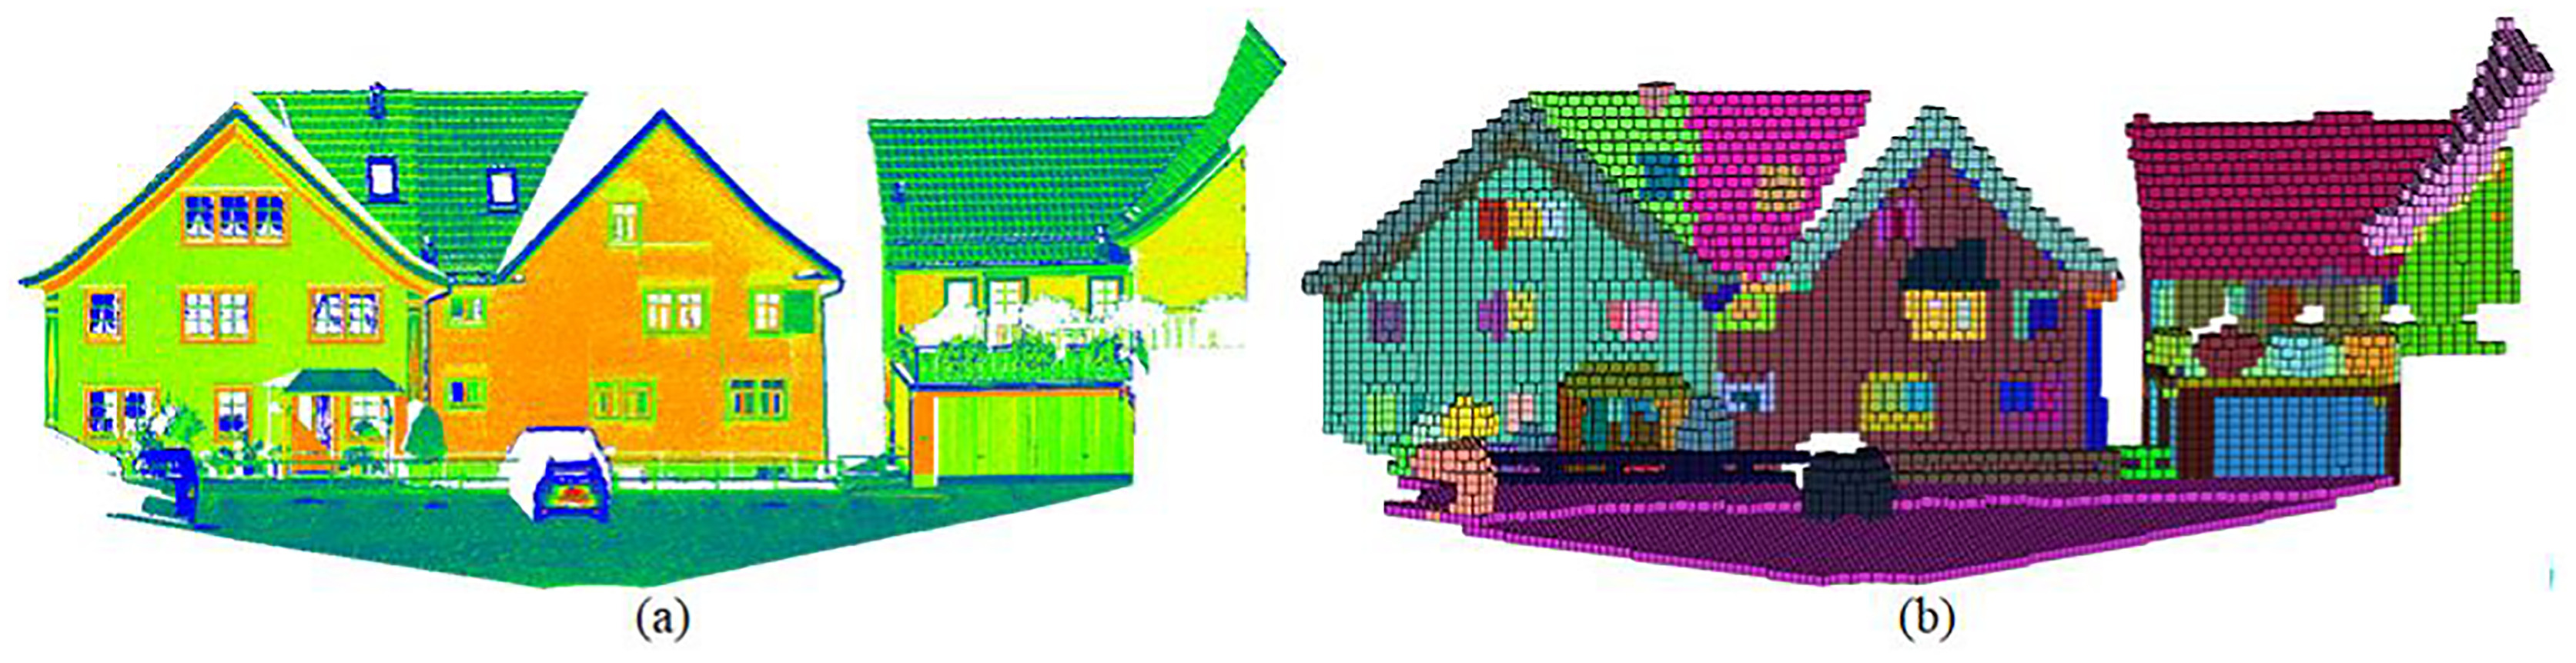
\includegraphics[width=15cm]{img/pc_vs_vox.jpg}
  \caption{Voxelová reprezentácia mračna bodov - (a) Originálne mračno bodov (b) Voxelová reprezentácia \cite{voxel_grid}}
  \label{voxel_example}
\end{figure}
\newline\indent Vo všeobecnosti, pri voxelizácií mračien bodov existujú štyri kroky. Prvý krok spočíva v výpočte ohraničenia mračna bodov, ktoré definuje priestor, ktorý sa má rozdeliť. V druhom kroku je definovaný priestor rastrovaný do pravidelných buniek tvaru kvádra s určitou veľkosťou. Potom je mračno bodov segmentované na malé časti týmito bunkami. Nakoniec sú rozdelené podmnožiny bodov reprezentované voxelmi, pričom sa z týchto bodov môžu vypočítať príslušné vlastnosti. \cite{voxel_grid}
\newline\indent Vďaka svojím vlastnostiam nachádzajú voxelové mriežky uplatnenie v mnohých oblastiach, ako sú predspracovanie údajov, modelovanie, registrácia, segmentácia a klasifikácia mračien bodov. 

\subsubsection{K-d strom}
\noindent K-d strom (k-dimenzionálny strom), je špecializovaná dátová štruktúra používaná na efektívnu organizáciu viacrozmerných dát. K-d strom funguje tak, že organizuje viacrozmerný priestor do hierarchickej binárnej stromovej štruktúry. Primárne sa používa na rýchle vyhľadávanie najbližšieho suseda, čo je kritická operácia v rôznych aplikáciách, ako je robotika, \acrshort{lidar} odometria a mapovanie a práca s mračnami bodov. \cite{kd_tree_new} \cite{kd_tree_old} 
\newline\begin{figure}[!htbp]
  \centering
  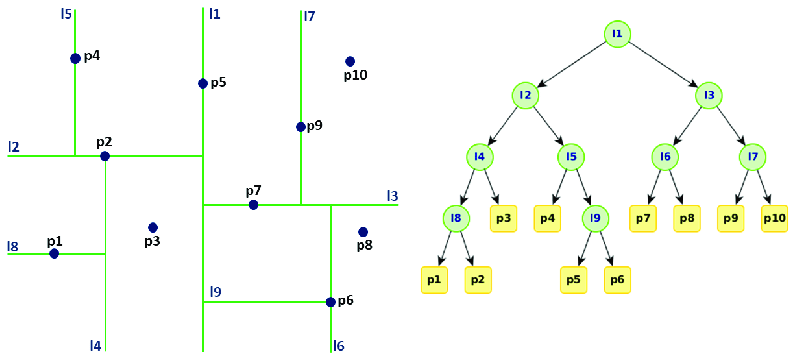
\includegraphics[width=14cm]{img/kd-tree.png}
  \caption{Reprezentácia k-d stromu v 2D priestore \cite{kd_tree}}
  \label{kd_tree}
\end{figure}
\newline\indent Vytvorenie k-d stromu spočíva v postupnom delení priestoru pozdĺž všetkých dimenzií, pričom ako bod delenia volíme hodnotu mediánu bodov v danom intervale. Tento spôsob vedie ku vzniku vyváženého stromu, až ku vzniku stromu, kde každá podmnožina obsahuje len jeden bod. Pri vytváraní stromu pomocou mediánu je časová zložitosť O(n log\textsubscript{2} n). Je možné použiť aj iné spôsoby rozdelenia ako medián, avšak tie nemusia vždy zabezpečiť rovnovážne vytvorenie stromu. \cite{kd_tree_old} 
\newline\indent Ako už bolo spomínané hlavným využitím k-d stromov v oblasti mračien bodov je vyhľadávanie najbližších susedov. Ak je už k-d strom vytvorený, algoritmus začína v koreni stromu a rekurzívne ním prechádza, pričom si vyberá vetvu, ktorá je najbližšie k zadanému bodu. Tento proces pokračuje, pokým sa nedosiahne listový uzol. Najbližší sused sa následne urči spätným pohybom po jednotlivých vetvách a kontrolovaním bližších susedov v ostatných vetvách. \cite{kd_tree_old}

\subsubsection{Oktálový strom}
\noindent Oktálový strom je dátová štruktúra navrhnutá na manipuláciu s 3D dátami, najmä mračnami bodov získaných zo zariadení ako laserové skenery. Organizuje priestor do kociek (alebo kvádrov), pričom každá kocka môže byť rozdelená na ďalších osem menších kociek. Oktánový strom je analógiou pre kvadrátový strom využívaný v 2D priestore. Kľúčovým konceptom tejto štruktúry je efektívne ukladanie dát prostredníctvom delenia priestoru len tam, kde sú existujúce body. \cite{oct_tree} 
\newline\begin{figure}[!htbp]
  \centering
  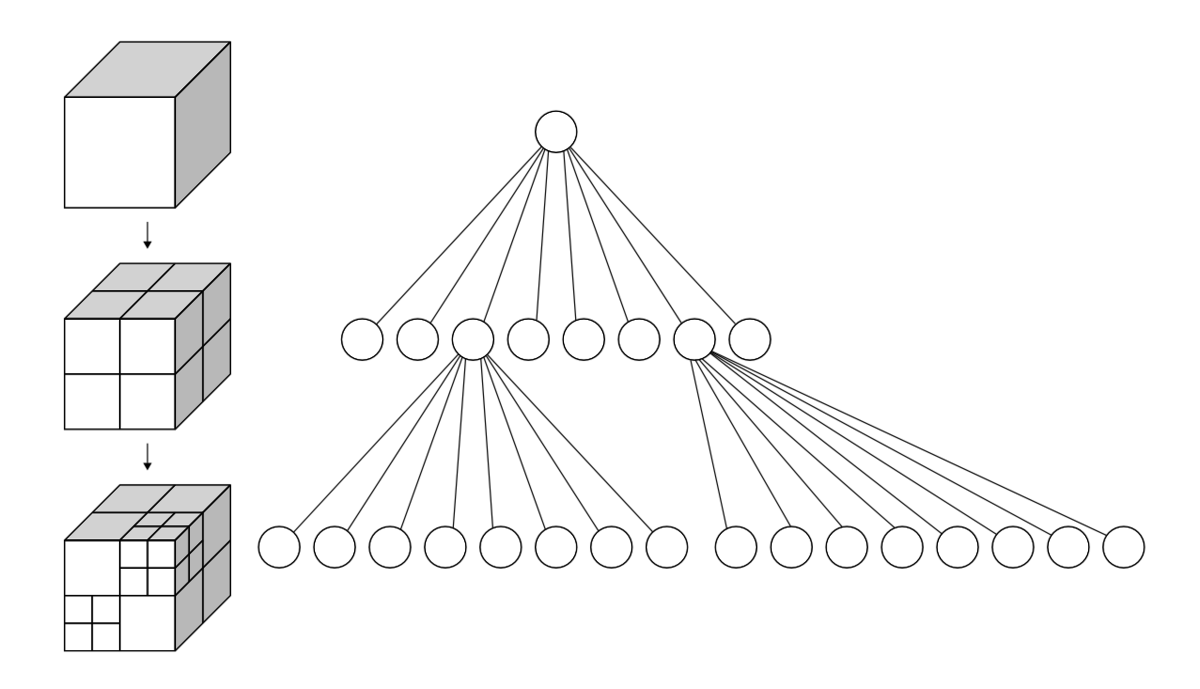
\includegraphics[width=12cm]{img/octree_full.png}
  \caption{Tradičná reprezentácia oktálového stromu \cite{oct_tree_img}}
  \label{oct_tree1}
\end{figure}
\newline\indent V procese tvorby oktálového stromu dochádza ku rekurzívnemu deleniu 3D priestoru na osem menších kociek, ktoré pokračuje až do splnenia určených zastavovacích podmienok. Tieto podmienky môžu zahŕňať dosiahnutie maximálnej úrovne delenia, čo zodpovedá najmenšiemu rozmeru kocky, alebo môžu byť viazané na minimálny počet bodov, pri ktorom delenie pokračuje. Kocky pre ktoré bolo delenie ukončené, sú označené ako tzv. listy a obsahujú informácie o všetkých príslušných bodoch. \cite{oct_tree}
\newline\indent Aj napriek tomu, že oktalový strom je považovaný za pamäťovo efektívnejšiu verziu voxelovej mriežky, má niekoľko nedostatkov, ktoré je možné vylepšiť. Optimalizovaná implementácia oktálového stromu eliminuje zbytočné dáta v pamäti a využíva ju efektívnejšie, pričom zachováva rýchle prístupové operácie. Na rozdiel od tradičných implementácií, ktoré ukladajú redundantné informácie o prázdnych bunkách, táto optimalizovaná verzia minimalizuje využívanie pamäte tým, že dynamicky pridáva pamäť len pre potrebné uzly a listy. Napriek zníženiu miesta v pamäti udržiava efektívne prístupové operácie z časovou zložitosťou O(log n). \cite{oct_tree}
\newline\begin{figure}[!htbp]
  \centering
  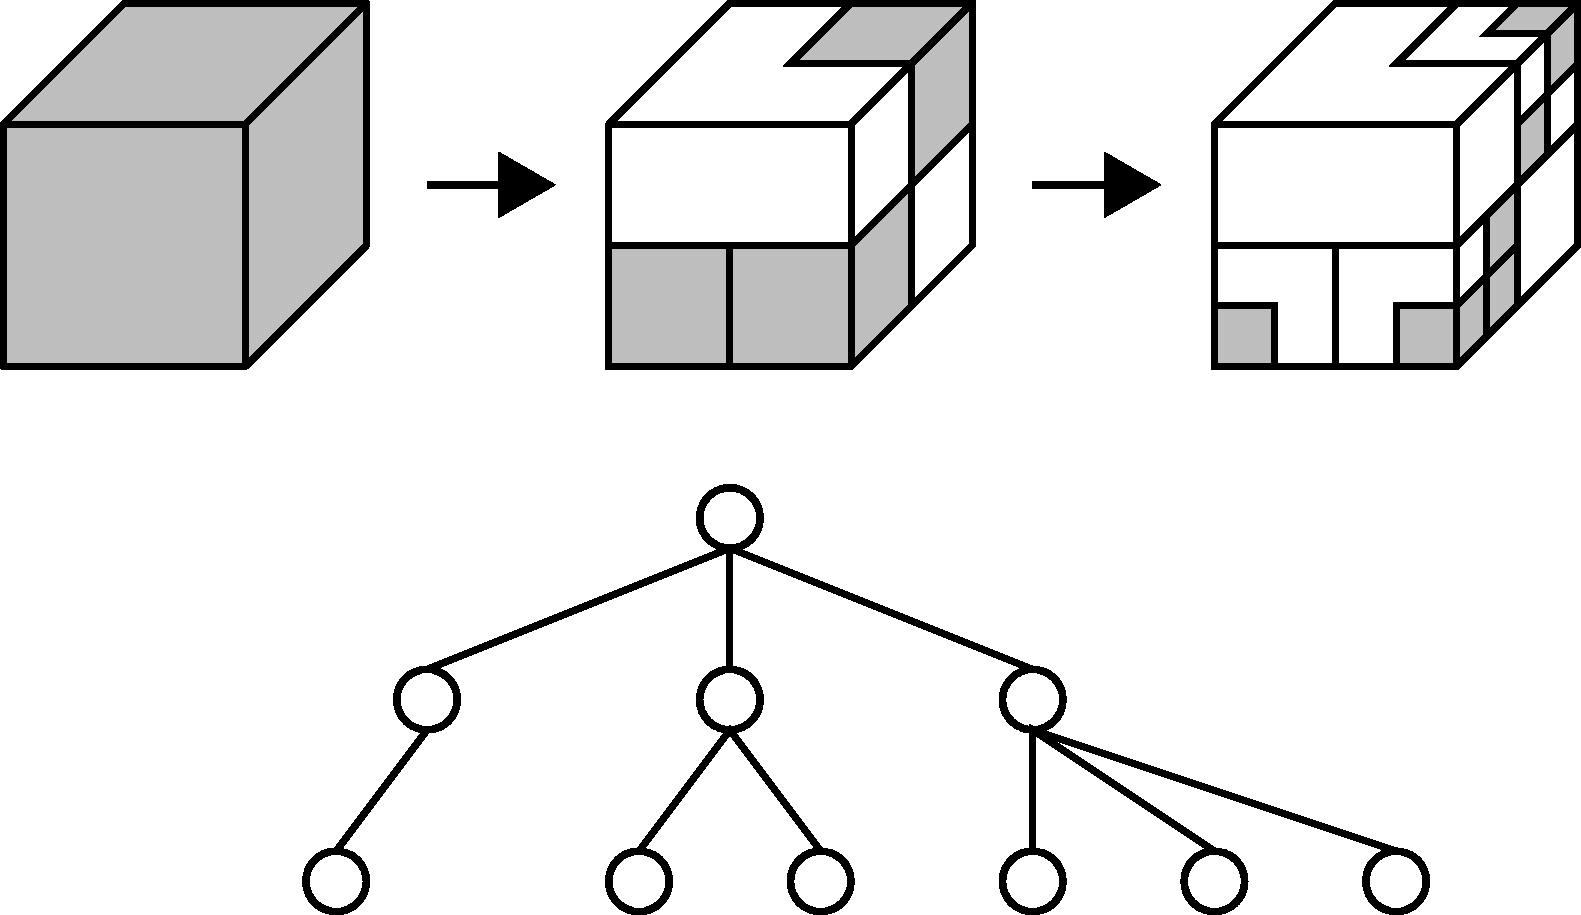
\includegraphics[width=11cm]{img/oct_tree_part.jpg}
  \caption{Optimalizovaná reprezentácia oktálového stromu (Bunky obsahujúce body označené šedou farbou) \cite{oct_tree}}
  \label{oct_tree2}
\end{figure}
\newline\indent Vďaka svojím vlastnostiam a efektívnej štruktúre nachádzajú oktálové stromy využitie v mnohých oblastiach, ako sú počítačové videnie, robotika, grafika a vizualizácia. V prípade robotiky a práce s mračnami bodov sa využívajú pre nájdenie najbližšieho suseda, ale aj kompresiu dát a podvzorkovanie.

\subsection{Filtrácia mračna bodov}
\noindent Mračná bodov získavané z rôznych typov senzorov, či už cenovo dostupných alebo drahých, často trpia prítomnosťou šumu a odľahlých hodnôt, ktoré sú výsledkom obmedzení samotných senzorov, vplyvu osvetlenia, či charakteru povrchu. Tieto nepresnosti vyžadujú využitie rôznych filtračných operácií, aby sa zabezpečila presnosť a vhodnosť pre ich ďalšie spracovanie. Prístupy filtrácie mračien bodov možno kategorizovať do niekoľkých skupín, medzi ktoré patria štatisticky založené metódy alebo metódy založené na susednosti. \cite{point_cloud_filtering}

\subsubsection{Štatisticky založené metódy} \label{section::sor}
\noindent Štatistické metódy detekcie odľahlých hodnôt spočívajú v použití štatistických konceptov na identifikáciu výnimočných (odlišných) hodnôt v súbore údajov. Využívajú koncepty, ako sú priemer, medián, štandardná odchýlka, kvartály a vzdialenosti, na identifikáciu hodnôt, ktoré sa výrazne odchyľujú od očakávanej distribúcie, čo naznačuje, že patria medzi odľahlé hodnoty. Medzi bežné metódy detekcie odľahlých hodnôt patria metódy ako Z-skóre, Chauvenetovo kritérium, Grubbsov test a Dixonov Q-test. 
\newline\indent Populárnou metódou pre filtrovanie mračien bodov je \acrshort{sor} (Statistical outlier removal). Metóda spočíva vo vypočítaní priemernej vzdialenosti medzi každým bodom a jeho \textit{K} najbližšími susedmi pomocou \acrshort{knn} algoritmu. Predpokladajúc, že tieto vzdialenosti nasledujú normálne rozdelenie, algoritmus aplikuje sigma pravidlo na základe zvoleného násobiteľa štandardnej odchýlky \textit{N}. A teda, ak priemerná vzdialenosť bodu a jeho susedov presahuje \textit{N} štandardných odchýlok priemernej vzdialenosti celého súboru, potom je bod považovaný za odľahlú hodnotu. Úpravou parametrov, ako je počet susedov \textit{K} a násobiteľ štandardnej odchýlky \textit{N}, je možné jemne nastaviť citlivosť algoritmu na odľahlé hodnoty. \cite{statistical_filter} 
\begin{figure}[!htbp]
  \centering
  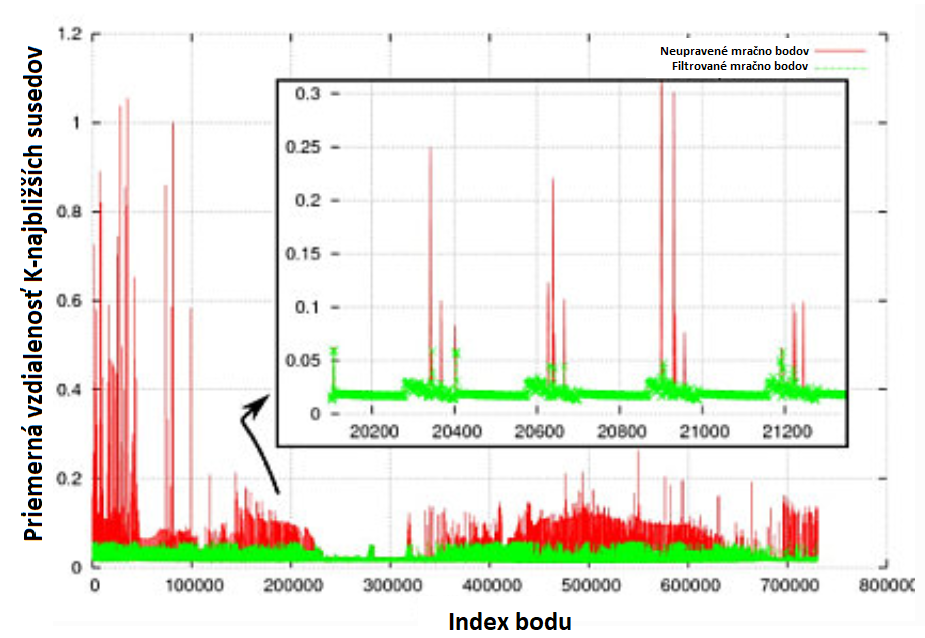
\includegraphics[width=14cm]{img/sor_principal.png}
  \caption{Princíp filtrovania odľahlých bodov pomocou \acrshort{sor} \cite{SOR_img}}
  \label{sor_principal}
\end{figure}

\subsubsection{Metódy založené na susednosti} \label{section::ror}
\noindent Metódy filtrovania založené na susedstve určujú vhodnosť bodu na základe jeho podobnosti s okolitými bodmi, čo výrazne ovplyvňuje účinnosť a efektivitu filtračného prístupu. Podobnosť medzi susednými bodmi môže byť definovaná ich vzájomnou vzdialenosťou, polohou, podobnosťou intenzity, farby alebo inými užitočnými vlastnosťami. \cite{point_cloud_filtering}
\newline\indent Jednou zo základných metód založených na susedstve je \acrshort{ror} (Radius outlier removal). Táto metóda je založená na určení minimálneho počtu susedov a polomeru v ktorom budú vyhľadávaní. Ak je počet nájdených susedov menší ako \textit{K}, je bod považovaný za odľahlý. Na Obr. \ref{ror_principal} môžeme vidieť princíp tejto metódy.
\begin{figure}[!htbp]
  \centering
  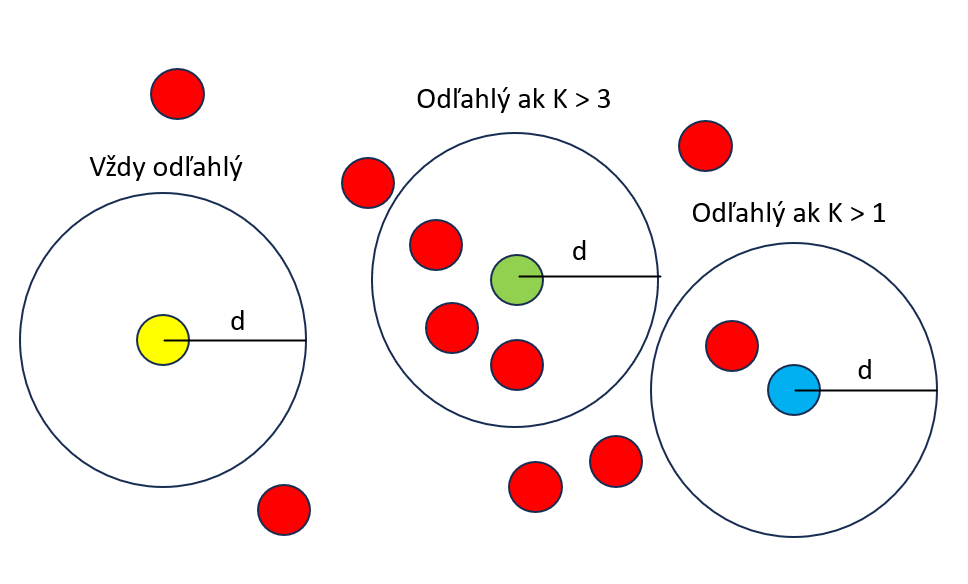
\includegraphics[width=12cm]{img/ros_principal.png}
  \caption{Princíp filtrovania odľahlých bodov pomocou \acrshort{ror} v 2D}
  \label{ror_principal}
\end{figure}

\newpage\subsection{Podvzorkovanie mračna bodov}
\noindent Metódy pre redukciu mračien bodov sú kľúčovým krokom pre zníženie pamäťových požiadaviek, zlepšenie výpočtovej efektívnosti a redukciu nežiaduceho šumu. Tieto metódy vo výsledku zmenšujú veľkosť mračien bodov, čo ich robí jednoduchšie pre manipuláciu, vizualizáciu a spracovanie. Snažia  sa dosiahnuť rovnováhu medzi znižovaním zložitosti a uchovaním kľúčových informácií, čo je podstatná vlastnosť pre ich ďalšie spracovanie. Vieme ich rozdeliť do dvoch základných skupín, bežné metódy a adaptívne metódy pre podvzorkovanie mračien bodov.

\subsubsection{Bežné podvzorkovacie metódy}
\noindent Bežné podvzorkovacie metódy obvykle vykonávajú rovnomerné alebo pravidelné zmenšenie počtu bodov. Tieto metódy nerozlišujú, akú úlohu napĺňajú jednotlivé body, čo môže viesť k potenciálnemu strateniu dôležitých čŕt alebo informácií v oblastiach, ktoré by mohli vyžadovať presnejšie podvzrokovanie.
\begin{enumerate}
  \item\textbf{Podvzorkovanie pomocou voxelovej mriežky} - Táto metóda rozdeľuje vstupné mračno bodov do voxelovej mriežky preddefinovaných rozmerov. Následne prechádza cez všetky vytvorené voxely, pričom ak voxel obsahuje aspoň jeden bod, bod najbližší ku ťažisku alebo samotné ťažisko reprezentuje všetky body vo voxely. Vstupným parametrom tejto metódy je veľkosť strán voxelu, čo ovplyvňuje úroveň zmenšenia a zachovaných detailov. Táto metóda dosahuje rovnomerné rozdelenie bodov v mračne, ale nezachováva potrebné detaily.
  \item\textbf{Náhodné podvzorkovanie} - Metóda náhodného podvzorkovania je založená na náhodnom výbere bodov z pôvodného mračna bodov, až do dosiahnutia stanoveného počtu. Napriek tomu, že táto metóda je jednoduchá a rýchla, nedosahuje rovnomerné rozdelenie bodov a nezachováva detaily, čo je obzvlášť pravda, ak má vstupné mračno bodov nerovnomernú hustotu. 
  \item\textbf{Rovnomerné podvzorkovanie} - Metóda spočíva v systematickom výbere bodov z pôvodného mračna s definovaným intervalom. Teda z celého mračna bodov vyberáme každý k-ty bod, čo znamená, že táto metóda je závislá od uloženého poradia bodov, a preto je vhodná, len pre určité mračná bodov. V prípade, že má vstupné mračno bodov nerovnomernú hustotu bodov, 
  výstupné mračno bude mať nerovnomerné rozdelenie.
  \item\textbf{Podvzorkovanie na základe najvzdialenejšieho bodu} - Táto metóda sa zameriava na dodržaní najväčšieho možného rozostupu bodov. Ako prvý sa vyberie náhodný bod, po čom sa iteratívne vyberá najvzdialenejší bod od aktuálneho vybraného, až dokým sa nedosiahne požadovaný počet bodov. Táto metóda dosahuje rovnomerné rozdelenie bodov a pri porovnaní s predošlými metódami, najlepšie opisuje geometriu objektov.
\end{enumerate}
\begin{figure}[!htbp]
  \centering
  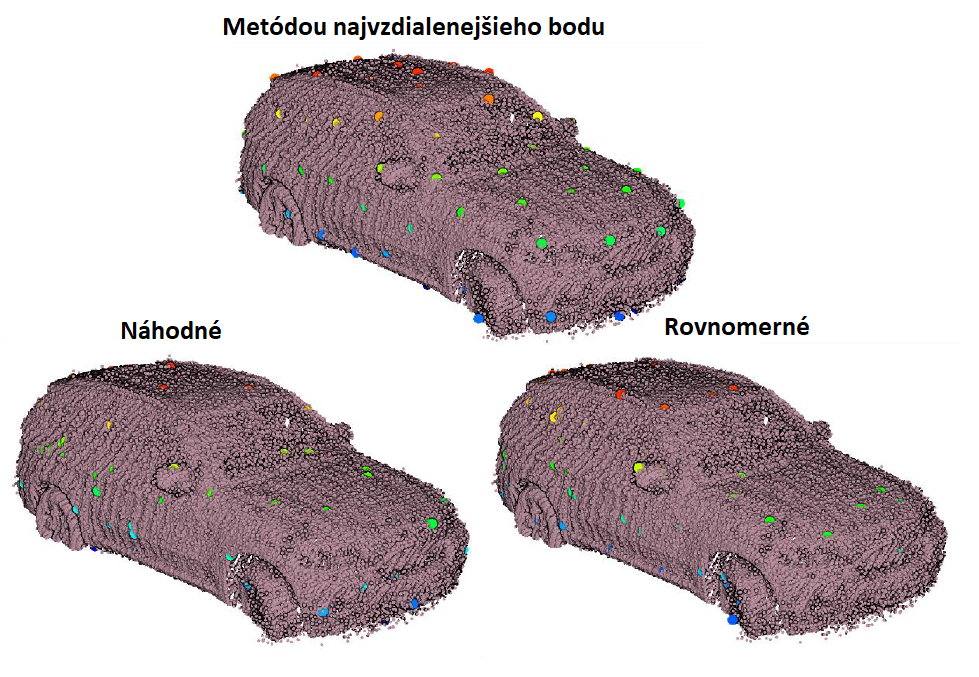
\includegraphics[width=15cm]{img/downsample.png}
  \caption{Ukážka rôznych metód podvzorkovania \cite{downsample_img}}
  \label{downsample}
\end{figure}

\subsubsection{Adaptívne podvzorkovacie metódy}
\noindent Adaptívne metódy podvzorkovania sa snažia zachovať dôležité body, ktoré opisujú detaily a zároveň efektívne odstrániť tie menej dôležité. Výber dôležitých bodov robia na základe viacerých charakteristík, pričom zohľadňujú faktory, ako lokálna hustota bodov, zakrivenie alebo iné geometrické vlastnosti.
\begin{enumerate}
  \item\textbf{Podvzorkovanie na základe krivosti} - Táto metóda využíva informácie o normálach alebo krivosti povrchu na určenie ich dôležitosti. Body vo rovnejších alebo menej zakrivených oblastiach môžu byť odstránené agresívnejšie, ako tie v oblastiach s vyššou krivosťou. Posudzovaním týchto geometrických vlastností je možné selektívne uchovávať body, ktoré prispievajú viac k celkovému tvaru alebo štruktúre objektu a zachovať dôležité detaily.
  \item\textbf{Podvzorkovanie na základe rovinnosti/susednosti} - Táto metóda využíva PCA (Principal Component Analysis) na charakterizáciu lokálnych susedstiev v mračnách bodov. PCA analyzuje vlastné čísla kovariančných matíc a zaraduje tieto susedstvá do troch hlavných kategórií: rovinné, lineárne/cylindrické alebo drsné. Po kategorizácii sa metóda zameriava na odhad hustoty bodov v každom type regiónu, pričom používa matematické vzorce prispôsobené individuálne pre každú kategóriu. Následne, na základe znalostí týchto susedstiev, môže selektívne preferovať odstránenie bodov v oblastiach, ktoré vykazujú rovinný charakter a majú hustotu bodov vyššiu, ako stanovenú užívateľom, zatiaľ čo v ostatných oblastiach aplikujeme menej agresívne podvzorkovanie. Pre lepšie pochopenie fungovania tejto metódy sa odkazujte na priložený článok. \cite{adaptive_downsampling_neighborhood}
\end{enumerate}
\begin{figure}[!htbp]
  \centering
  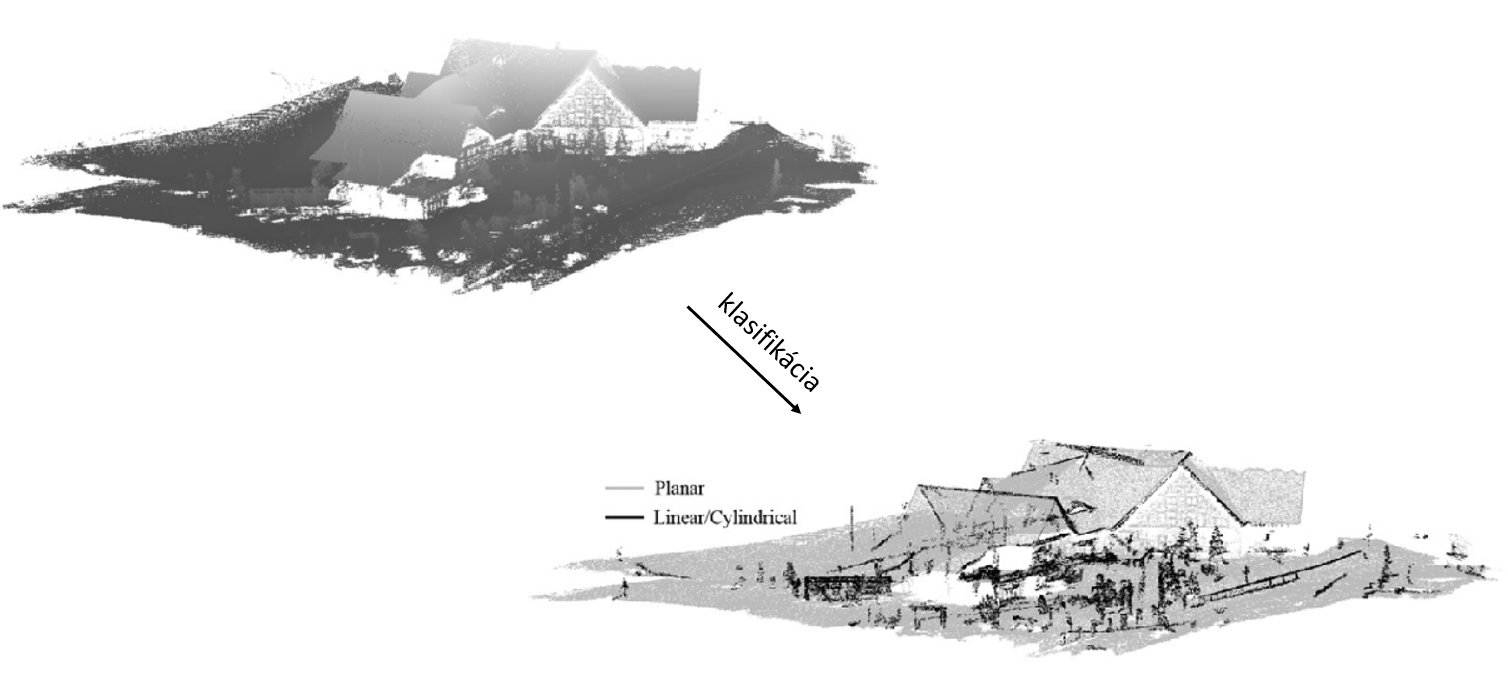
\includegraphics[width=15cm]{img/planar_example.png}
  \caption{Ukážka klasifikácie dôležitých bodov pomocou metódy založenej na rovinnosti \cite{adaptive_downsampling_neighborhood}}
  \label{noname}
\end{figure}

\subsection{Segmentácia}
\noindent Segmentácia je proces rozdelenia väčšieho celku údajov na menšie významovo odlišné časti, na základe určitých charakteristík alebo vlastností. V kontexte mračien bodov alebo počítačového videnia, segmentácia rozdeľuje údaje na jednotlivé časti, na základe vlastnosti, ako sú farba, textúra, geometria a ďalšie. V prípade mračien bodov pomáha segmentácia rozlíšiť rôzne objekty alebo povrchy v scéne, čím pomáha pri úlohách, ako klasifikácia objektov, rekonštrukcia povrchu, navigácia robotov. Celkovo segmentácia slúži, ako základný krok pri extrahovaní významných informácií zo scény, čo umožňuje hlbšiu analýzu, porozumenie a využitie segmentovaných komponentov pre ďalšie účely. 
\subsubsection{Segmentačné metódy}
\noindent V tejto podkapitole preskúmame rôzne prístupy navrhnuté pre segmentáciu mračien bodov, pričom ich vieme rozdeliť do piatich zakladných kategórií (Obr. \ref{segmentation_methods}).
\begin{figure}[!htbp]
  \centering
  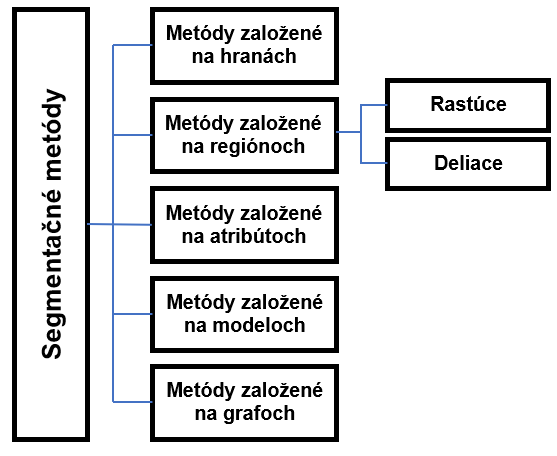
\includegraphics[width=11cm,height=7.5cm]{img/segmentation_methods.png}
  \caption{Rozdelenie segmentačných metód}
  \label{segmentation_methods}
\end{figure}
\begin{enumerate} 
 \item\textbf{Metódy založené na hranách} - Tieto metódy sa zameriava na detekciu hrán, pomocou rôznych prístupov, ako sú identifikácia výrazných zmien intenzity, zmien orientácie normálových vektorov alebo výpočtu gradientu. Tieto metódy zvyčajne pozostávajú z dvoch fáz. Prvou je detekcia hrán, kde sa vytvárajú obrysy hraníc regiónov na základe lokálnych zmien vlastností povrchu, pričom v druhej fáze sa vnútorne body zoskupia, čím sa vytvoria samostatné segmenty. Aj keď tieto metódy umožňuje rýchlu segmentáciu, často sa stretávajú s problémami presnosti kvôli citlivosti na šum a variáciám hustoty mračien bodov. V 3D priestore môžu detegovať nespojité hrany, čo komplikuje identifikáciu uzavretých segmentov bez ďalších dodatočných krokov. \cite{segmetation_survey} 
 \item\textbf{Metódy založené na regiónoch} - Metódy založené na regiónoch využívajú informáciu o okolitých bodoch s podobnými vlastnosťami na vytvorenie izolovaných regiónov a následne zisťujú odlišnosti medzi týmito regiónmi. Metódy založené na regiónoch sú odolnejšie voči šumu, ako metódy založené na hranách, avšak majú problém s nadmerným alebo nedostatočným segmentovaním a presným určovaním hraníc regiónov. Tieto metódy delíme do dvoch kategórií:  \cite{segmetation_survey} 
 \begin{itemize}
    \item\textbf{Rastúce} (z ang. seeded-region) začínajú výberom určitého počtu začiatočných bodov, a z týchto bodov následne každý región rastie pridaním susedných bodov, ak spĺňajú určité kritériá kompatibility. Medzi tieto kritéria patrí vzdialenosť, intenzita alebo rovnosť susedných bodov. \cite{segmetation_survey}  
    \item\textbf{Deliace} (z ang. unseeded-region) najprv zoskupia všetky body do jedného regiónu. Potom začína proces delenia na menšie regióny a pokračuje, až pokým zvolená miera vhodnosti presahuje stanovený prah. \cite{segmetation_survey}
 \end{itemize}
 \item\textbf{Metódy založené na atribútoch} - Tieto metódy využívajú vypočítané charakteristiky (atribúty) jednotlivých bodov, ako sú priestorové súradnice, hustota, povrchová textúra a ďalšie, na zoskupovanie podobných bodov. Tieto atribúty usmerňujú zhlukovacie algoritmy, ktoré vytvárajú odlišné segmenty na základe podobnosti atribútov s cieľom izolovať rôzne povrchy alebo objekty v mračne bodov. Aj keď sú tieto metódy flexibilné a presné, ich presnosť silno závisí od presnosti odvodených atribútov.
 \item\textbf{Metódy založené na modeloch} - Tieto metódy sa snažia nájsť a kategorizovať body na základe ich reprezentácie pomocou základných tvarov. Využívajú základné geometrické tvary, ako guľa, kužeľ, rovina a valec na zoskupovanie bodov s podobnými matematickými vlastnosťami. Sú rýchle a robustné voči šumu, ale môžu sa stretnúť s problémami pri práci s rôznorodými alebo komplexnými mračnami bodov. \cite{ransac}
 \item\textbf{Metódy založené na grafoch} - Tieto metódy vnímajú body, ako vzájomne prepojené vrcholy pomocou hrán, pričom hrany reprezentujúce vzťahy medzi susediacimi bodmi. Využívajú štruktúry grafov, kde zohľadňujú rôzne kritériá, ako sú farba, normály alebo pravdepodobnostné modely. Tieto metódy sú známe svojou presnosťou a efektívnosťou, najmä v robotických aplikáciách. Napriek tomu, že sú schopné pracovať so šumom alebo rôznorodými dátami, môžu čeliť problémom s spracovaním v reálnom čase a často vyžadujú predchádzajúce znalosti alebo špecializované nastavenia senzorov. \cite{segmetation_survey}\cite{graph_based}
\end{enumerate}

\subsubsection{DBSCAN}
\noindent \acrshort{dbscan} (Density-Based Spatial Clustering of Applications with Noise) je populárny zhlukovací algoritmus, používaný pre analýzu priestorových dát a segmentáciu mračien bodov. Tento algoritmus využíva princíp toho, že zhluky sú oblasti s vysokou hustotou, oddelené miestami s nižšou hustotou bodov. Algoritmus dynamicky identifikuje zhluky na základe hustoty bodov, bez predpokladu fixného počtu zhlukov alebo konkrétnych tvarov. \cite{DBSCAN_original} 
\newline\indent \acrshort{dbscan} pracuje s dvomi vstupnými parametrami: \textit{Eps} a \textit{MinPts}. \textit{Eps} definuje polomer prehľadávaného okolia, zatiaľ čo \textit{MinPts} určuje minimálny počet bodov v rámci \textit{Eps} potrebných na vytvorenie hustej oblasti. Nastavenie týchto parametrov je kľúčové pre správne fungovanie algoritmu, a preto existuje heuristika, ktorá ich určuje na základe ``najtenšieho'' zhluku, ktorý nie je považovaný za šum. \cite{DBSCAN_original}
\newline\indent Princíp fungovania algoritmu vieme rozdeliť do niekoľkých bodov:
\begin{enumerate}
    \item Pre každý bod zo súboru sa vypočíta počet bodov ležiacich v okolí určeným \textit{Eps} hodnotou. Na základe tejto hodnoty sú body zaradené do troch kategórií.  
    \item Body, ktoré majú tento počet väčší, ako hraničná hodnota \textit{MinPts} sú považované za jadrové, naopak tie ktoré ju majú menšiu, ale zároveň sú  v \textit{Eps} okolí iného jadrového bodu, sú považované za hraničné. Zvyšné body sú zaradené medzi šumové.
    \item Následne sa vytvárajú zhluky pomocou spájania jadrových bodov, ktoré ležia vo svojom \textit{Eps} okolí, pričom sú ohraničené hraničnými bodmi. Body šumu nie sú zaradené do žiadnych zhlukov.
\end{enumerate}

\subsubsection{K-means}
\noindent K-means je populárny algoritmus pre zhlukovanie súborov dát, ktorý rozdeľuje dáta do \textit{K} odlišných a neprekrývajúcich sa zhlukov. Jeho cieľom je minimalizovať rozptyl vzdialeností vo vnútri zhlukov prostredníctvom iteratívneho priraďovania bodov ku najbližšiemu centru, pričom centrá zhlukov, sú aktualizované, až do dosiahnutia konvergencie. \cite{K-means}
\newline\indent Princíp fungovania algoritmu vieme rozdeliť do niekoľkých bodov:
\begin{enumerate}
    \item Výber K náhodných bodov zo súboru a označenie ich za centrá. 
    \item Následne sa všetky body priraďujú ku svojmu najbližšiemu centru.
    \item Zo priemeru združených bodov sa vypočíta nové centrum.
    \item Predošlé body sa opakujú až dokým jednotlivé centrá nezkonvergujú do svojej optimálnej  polohy (ich poloha sa už výrazne nemení).
\end{enumerate}
\indent Aj napriek tomu, že K-means algoritmus má jednoduchý princíp fungovania, náhodný výber počiatočných centier môže viesť ku uväzneniu v lokálnom minime, a pre optimálny výsledok, je potrebné, aby bol algoritmus spustený niekoľkokrát. Určenie správneho počtu zhlukov \textit{K} predstavuje ďalší problém. S rastúcim \textit{K} klesá rozptyl, ktorý sa snažíme minimalizovať. Aby sa zabránilo jeho nekonečnému nárastu existuje tzv. lakťová metóda (z ang. elbow method), pri ktorej z grafu pre rôzne hodnoty \textit{K} vieme nájsť zlom, pri ktorom rozptyl začne klesať výrazne pomalšie. \cite{K-means}
\begin{figure}[!htbp]
  \centering
  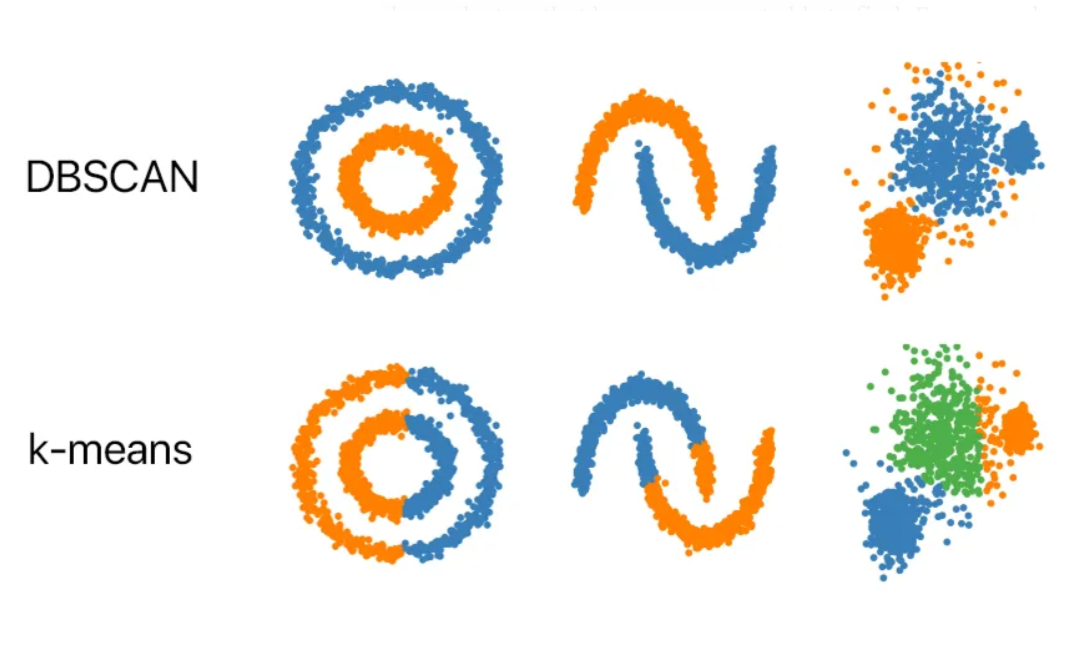
\includegraphics[width=13cm]{img/DBSCAN_vs_Kmeans.png}
  \caption{Porovnanie segmentácie pomocou DBSCAN a K-means algoritmu \cite{DBSCANvsKmeans}}
  \label{DBSCAN_vs_Kmeans}
\end{figure} 

\subsubsection{RANSAC}
\noindent \acrshort{ransac} (Random Sample Consensus) je metóda používaná na odhad parametrov matematického modelu zo súboru dát, ktorý môže obsahovať odľahlé hodnoty alebo chyby. Na rozdiel od tradičných metód, ktoré sa snažia zahrnúť väčšinu údajov a eliminovať odľahlé hodnoty, \acrshort{ransac} funguje tým, že začína s minimálnym množstvom údajov a postupne ho rozširuje o konzistentné údaje na vytvorenie spoľahlivého modelu. \cite{RANSAC_original}
\newline\indent Metóda začína výberom \textit{N} bodov zo celého súboru, pričom \textit{N} predstavuje najmenší potrebný počet bodov pre vyjadrenie modelu. Následne sa pre vybrané body vypočítava zvolený model (napr. priamka, krivka, plocha). Pre daný model sa identifikujú body, ktoré súhlasia s modelom v rámci definovanej tolerancie a zaznamenáva sa ich počet. Tieto kroky sa iteratívne opakujú, až do dosiahnutia definovaného počtu iterácií, alebo až kým nie je splnená ukončovacia podmienka (napr. nájdenie modelu s dostatočným počtom bodov). Ak je identifikácia ukončená nájdením dostatočného počtu bodov, \acrshort{ransac} využíva vyhladzovaciu techniku, ako je napríklad metóda najmenších štvorcov, na výpočet vylepšeného odhadu parametrov modelu zo všetkých príslušných bodov. \cite{RANSAC_original}
\begin{figure}[!htbp]
  \centering
  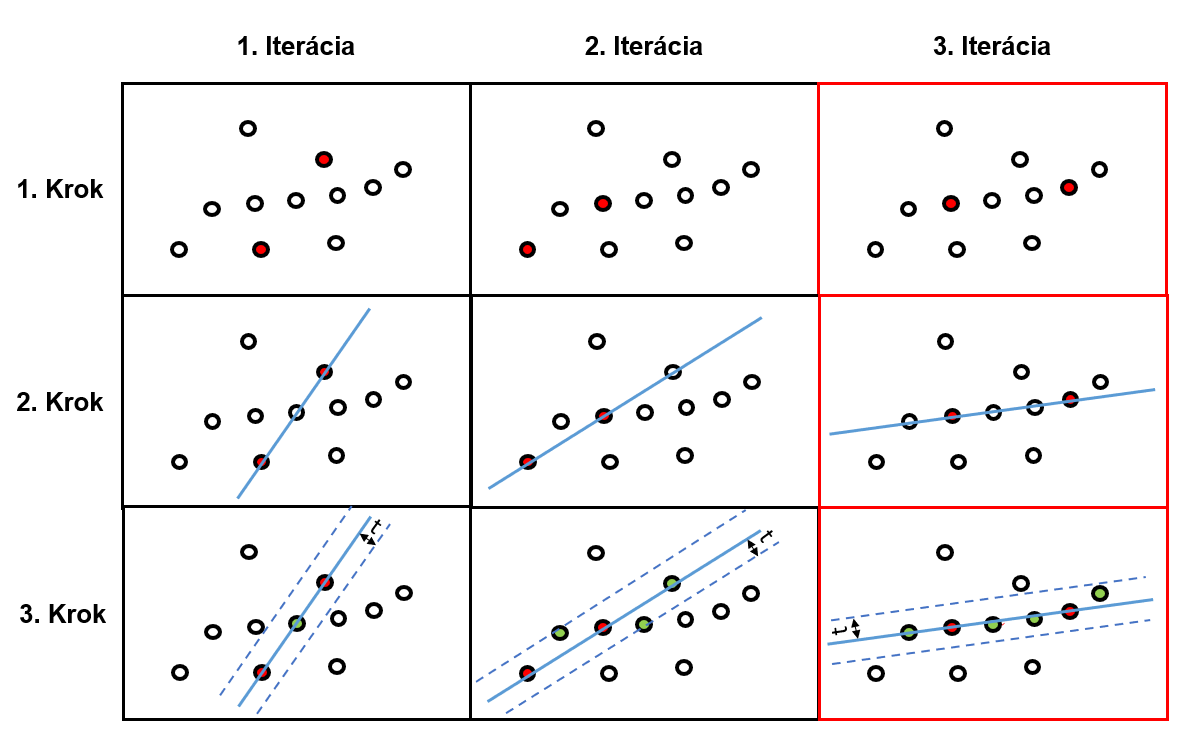
\includegraphics[width=16cm]{img/ransac_img.png}
  \caption{Postup \acrshort{ransac} algoritmu pre odhad parametrov modelu priamky}
  \label{ransac}
\end{figure} 

\section{Rekonštrukcia a spracovanie povrchu}
\noindent Rekonštrukcia povrchu, či už z fotiek alebo mračien bodov, sa stala v posledných rokoch populárnou témou vďaka rýchlemu vývoju výpočtovej techniky, ale aj cenovému sprístupneniu skenerov, ktoré ponúkajú slušné výsledky. Tento proces nachádza vysoké využitie v oblastiach, ako sú robotika, počítačová vízia, mapovanie, ale aj kultúrne dedičstvo. V týchto oblastiach sa stretávame so scénami, ktoré obsahujú objekty so rôznymi rozmermi, a zachovanie presnosti a zníženie pamäťovej náročnosti je náročnou a dôležitou úlohou. Pre tento účel sa vyvinulo mnoho rôznych metód, ktoré majú svoje výhody aj nevýhody.
\begin{figure}[!htbp]
  \centering
  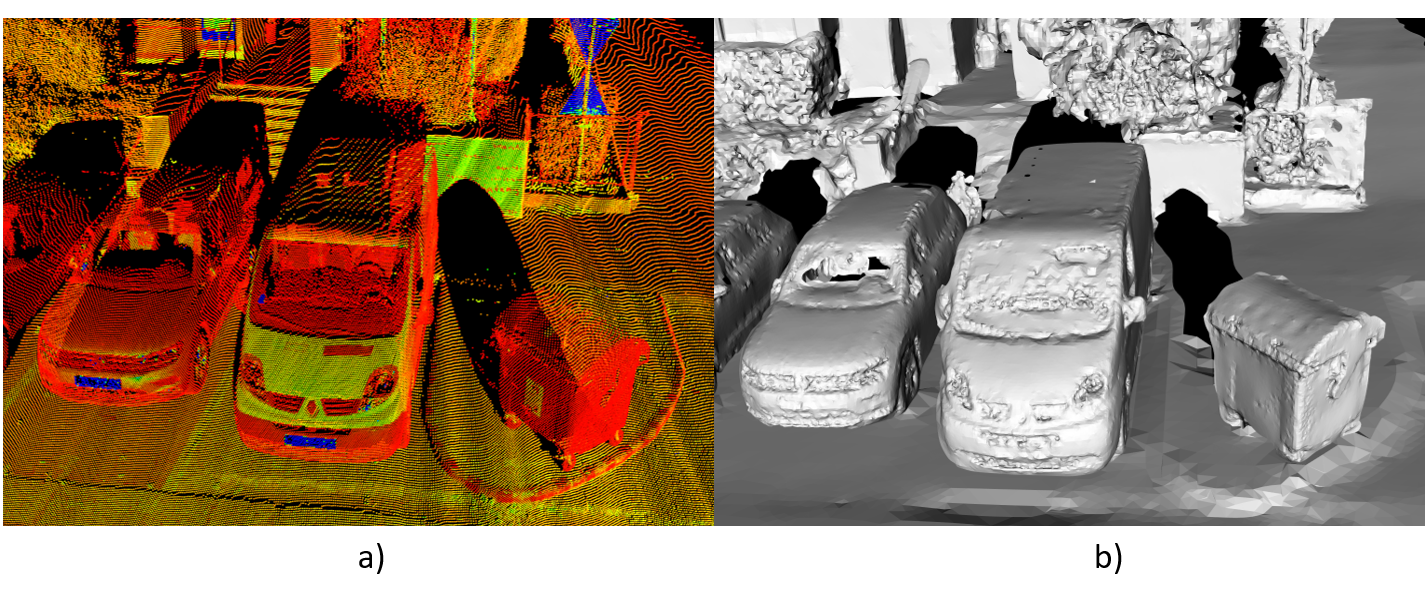
\includegraphics[width=16cm, height=8cm]{img/mesh_example.png}
  \caption{Ukážka rekonštrukcie povrchu - (a) mračno bodov (b) zrekonštruovaný povrch}
  \label{recons}
\end{figure} 
\newline\indent Jednotlivé metódy vieme rozdeliť do dvoch základných skupín na základne ich prístupu, ku generovaniu povrchu.
\begin{enumerate}
    \item\textbf{Explicitné metódy} - Využívajú explicitnú reprezentáciu povrchu (primitívne tvary), čo znamená, že vytvorený povrch bude ležať priamo na bodoch mračna. Ich nevýhodou je vysoká citlivosť na šum, ako aj časová náročnosť na výpočet.
    \item\textbf{Implicitné metódy} - Využívajú Implicitnú reprezentáciu povrchu, a teda povrch je charakterizovaný funkciami, ktorých izo-kontúry tesne aproximujú body mračna. Rekonštrukcia implicitných plôch spočíva vo vyhľadávaní funkcie, ktorá najlepšie vyhovuje vstupným bodom, pričom následne vyžaduje dodatočné spracovanie pre vizualizáciu. Metóda Marching Cubes patrí medzi najpoužívanejšie metódy pre generovanie trojuholníkových plôch z implicitnej reprezentácie. \cite{Reconstruction_general}
\end{enumerate}

\subsection{Metódy pre rekonštrukciu povrchu}
\noindent V tejto podkapitole sa zameriame na principiálne fungovanie konkrétnych metód pre rekonštrukciu povrchu. Ako už bolo povedané, metódy delíme na explicitné a implicitné, pričom väčšina z uvedených metód bude implicitná, nakoľko sú odolnejšie voči šumu a výpočtovo menej náročné. 
\subsubsection{Marching cubes} \label{sec:marching_cubes}
\noindent Metóda marching cubes je jednou z najpoužívanejších metód pre rekonštrukciu povrchu. Táto metóda je založená rozdelení priestoru do voxelovej mriežky, pričom každý voxel tvorí osem vrcholov. Každému vrcholu je priradená hodnota podľa toho, či sa nachádza vnútri (hodnota 1) alebo mimo prehľadávaného povrchu (hodnota 0), podľa hraničnej úrovne nastavenej od užívateľa. Pre osem vrcholov existuje 256 rôznych konfigurácii, čo môže byť pomerne zložité na spracovanie. Preto sa tieto konfigurácie redukujú na 14 vzorov (Obr. \ref{marchingCubes}) vďaka symetrickým vlastnostiam, čím sa zároveň minimalizuje pravdepodobnosť chýb. \cite{MarchingCubeas_origin}
\newline\indent Výhodou tejto metódy je, že pre svoju funkciu nepotrebuje odhad normál, ale naopak, pôvodná verzia ponúka výpočet normál pomocou gradientu. Tieto normály je možno následne využiť pri vizualizácií a tieňovaní výsledného povrchu. Na druhú stranu jednou z hlavných nevýhod je využitie voxelovej mriežky, čo môže pri veľkých mračnách bodov viesť, ku rýchlemu naplneniu RAM pamäte. Pre odstránenie tohto problému je nutná úprava pôvodnej metódy, ktorá rozdelí prehľadávaný priestor na viacero častí a na konci ich spojí.
\begin{figure}[!htbp]
  \centering
  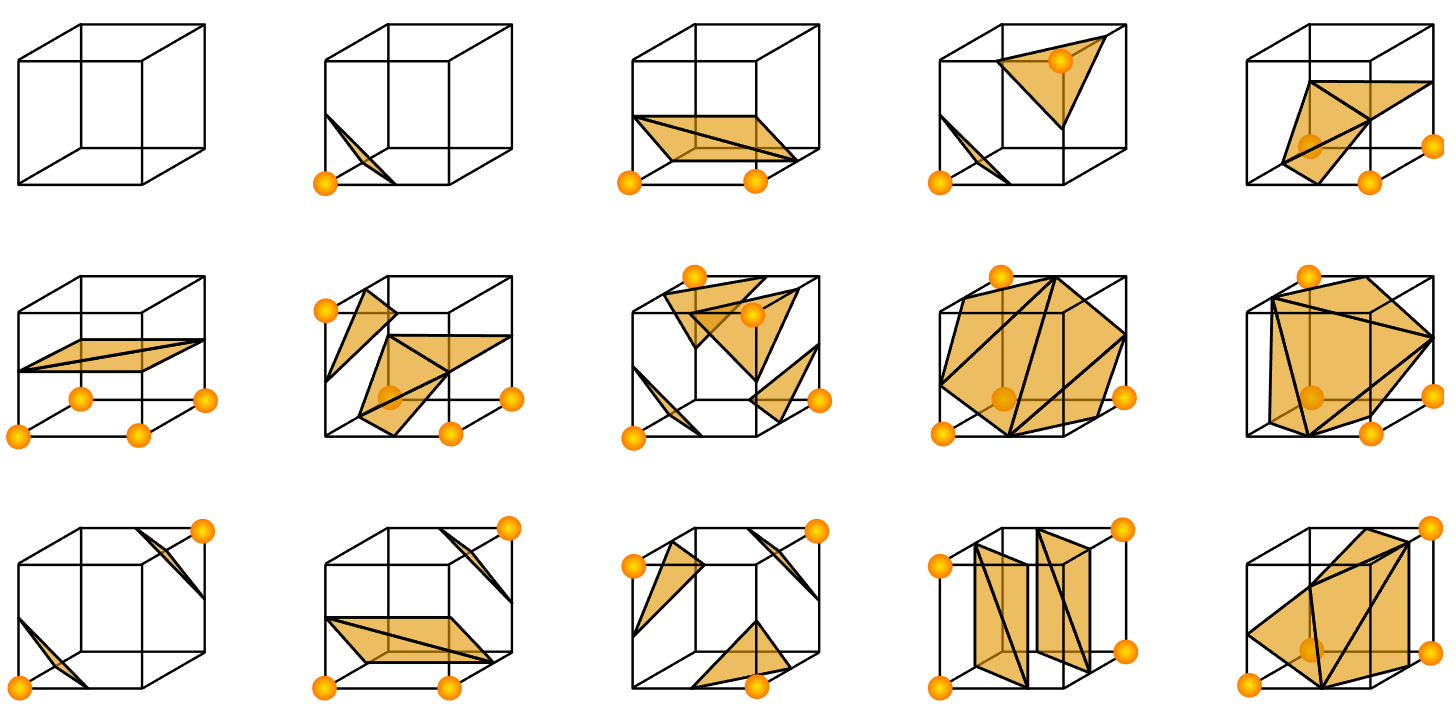
\includegraphics[width=16cm, height=8.5cm]{img/marching_cubes.png}
  \caption{Rôzne možnosti konfigurácie voxelov \cite{MarchCubes_img}} 
  \label{marchingCubes}
\end{figure} 
\subsubsection{Poisson} \label{sec:poisson}
\noindent Táto metóda ukazuje, že rekonštrukciu povrchu z orientovaných bodov môže byť vyriešená, ako priestorový Poissonov problém. Formulácia pomocou Poissonovej metódy zohľadňuje všetky body naraz, bez použitia heuristického priestorového delenia alebo prelínania, a je preto vysoko odolná voči šumu. \cite{poisson_origin}
\newline\indent Táto metóda využíva implicitný prístup pre reprezentáciu povrchu, konkrétne sa zameriava na výpočet 3D indikačnej funkcie $\chi$ (definovanej, ako 1 pre body vnútri modelu a 0 pre body mimo modelu viď Obr. \ref{fig:poisson}) a následne získanie zrekonštruovanej plochy extrahovaním vhodnej izo-kontúry. Dôležitým poznatkom je, že medzi orientovanými bodmi získanými z povrchu modelu a indikačnou funkciou modelu, existuje integrálny vzťah. Konkrétne, gradient indikačnej funkcie je vektorové pole, ktoré je nulové takmer všade (keďže funkcia indikátora je konštantná takmer všade), okrem bodov blízkych povrchu, kde je rovné normálam smerujúcim do vnútra povrchu. S tohto dôvodu, vzorky orientovaných bodov možno považovať za vzorky gradientu indikačnej funkcie modelu. \cite{poisson_origin}
\begin{figure}[!htbp]
  \centering
  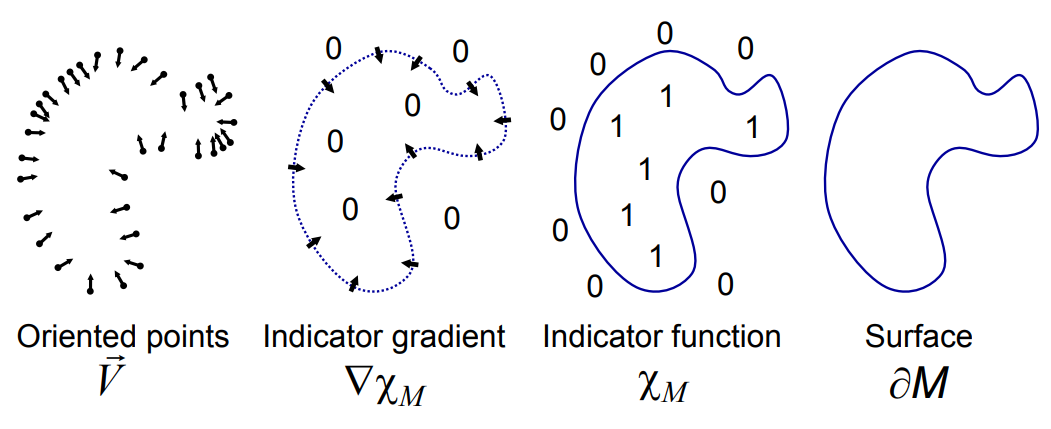
\includegraphics[width=14cm]{img/poisson.png}
  \caption{Ukážka Poissonovej rekonštrukcie v 2D \cite{poisson_origin}} 
  \label{fig:poisson}
\end{figure} 
\newline\indent Úloha výpočtu indikačnej funkcie sa zjednodušuje na hľadanie skalárnej funkcie $\chi$, ktorej gradient najlepšie aproximuje dané vektorové pole $\vec{V}$, definované množinou vzoriek. Keď sa použije operátor divergencie, táto úloha sa pretransformuje do štandardného Poissonového problému, kde je cieľom vypočítať $\chi$, tak aby jeho Laplacián (divergencia gradientu), bol rovný divergencii vektorového poľa $\vec{V}$. \cite{poisson_origin}
\begin{equation}
    \Delta \chi \equiv \nabla \cdot \nabla \chi = \nabla \cdot \vec{V}
    \label{eq:poisson}
\end{equation}
\indent Ako už bolo skôr uvedené, táto metóda vytvára globálne riešenie, ktoré využíva všetky body naraz. To jej umožňuje vytvoriť vodotesný a hladký povrch, čo môže byť výhoda oproti iným metódam. Naopak metóda potrebuje na vstup orientované body a je teda nutné mať informáciu o normálach, čo môže byť problém, ak je rekonštruovaný objekt nasnímaný z viacerých snímkov.   

\subsubsection{Ball pivoting}
\noindent Hlavný princíp fungovania tejto metódy, je celkom jednoduchý. Uvažujme body v priestore, na ktoré položíme $\rho$-guľu (guľa s rádiusom $\rho$), pričom uvažujeme, že hustota bodov je dostatočne veľká na to, aby cez nich guľa nevedela prejesť bez dotyku. Metóda začína rekonštrukciu položením $\rho$-gule na povrch, tak aby sa dotýkala troch náhodných bodov. Následne sa guľa udržuje v kontakte s dvoma pôvodnými bodmi a obtáča sa (z ang. pivot), až dokým nenarazí na ďalší bod. Trojica bodov, s ktorými je guľa v kontakte, tvorí nový trojuholník a pridáva sa ku existujúcemu povrchu. Proces sa opakuje prechádzaním po okraji súčasnej hranice povrchu, až dokým neboli prejdené všetky hranice a nepribudol žiadny nový trojuholník. \cite{ball_pivot_origin}
\newline\indent Aj napriek jednoduchosti a priamočiarosti, má táto metóda svoje nedostatky. Ako môžeme vidieť na Obr. \ref{fig:ball_pivot}, metóda funguje dobre, ak pracuje v ideálnych podmienkach. V prípade, ak sú body neuniformné (častí prípad mračien bodov), guľa nedokáže premostiť ku ďalšiemu bodu a v povrchu vznikajú diery. Rovnaký prípad nastáva, aj keď je polomer gule príliš veľký a rekonštruovaný objekt obsahuje detaily s príliš veľkým zakrivením.
\begin{figure}[!htbp]
  \centering
  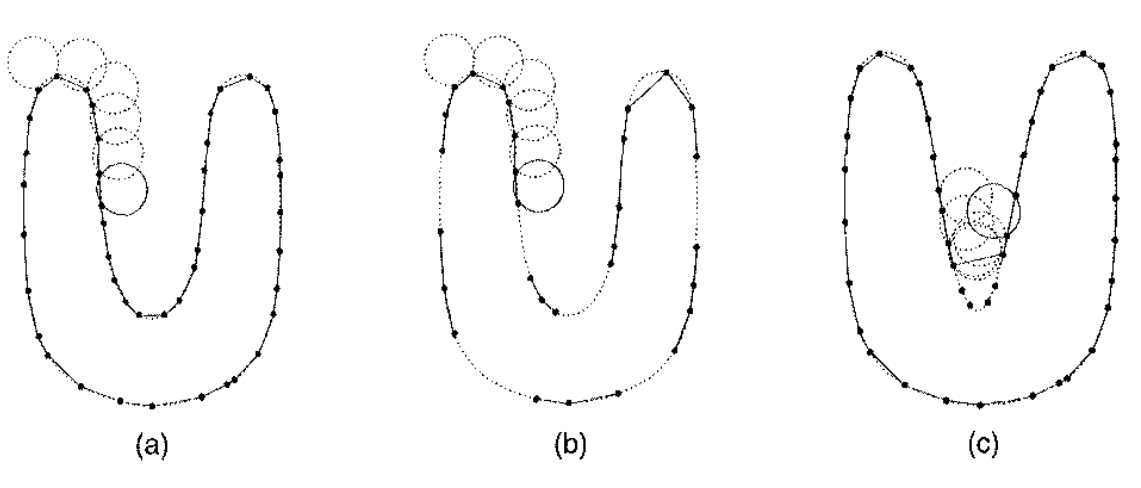
\includegraphics[width=16cm]{img/ball_pivoting.png}
  \caption{Ukážka ball-pivoting rekonštrukcie v 2D - (a) Ideálny prípad (b) mála a neuniformná hustota bodov (c) príliš veľké zakrivenie (väčšie ako 1/$\rho$) \cite{poisson_origin}} 
  \label{fig:ball_pivot}
\end{figure} 

\subsubsection{MLS}
\noindent \acrshort{mls} (Moving least squares) je trieda, ktorá zastrešuje viacero metód, ktoré pristupujú ku rekonštrukcií povrchu, tak že aproximuje jednotlivé body pomocou polynómu nízkeho rádu (kubický, kvadratický), čo zároveň ponúka možnosť podvzorkovania alebo nadvzorkovania. \cite{MLS_survey}
\newline\indent Za predpokladu, že skalárna hodnota $v_i$, je priradená ku každej vstupnej vzorke $p_i$, je potom zrekonštruovaná plocha v $x$ definovaná, ako hodnota v $x$ viacrozmerného polynómu $g_x$, ktorý najlepšie aproximuje susedstvo bodu $x$ v zmysle váženej metódy najmenších štvorcov \cite{MLS_survey}:
\begin{equation}
    g_x = \arg\min_{g}\sum\omega(||x-p_i||)(g(p_i)-v_i)^2
    \label{eq:mls}
\end{equation}
\indent kde $\omega$ je váhová funkcia, ktorá priraďuje väčší vplyv bodom, ktoré sú bližšie ku aktuálne hodnotenému bodu. Táto váhová funkcia taktiež pôsobí, ako forma dolnopriepustného filtra, pomáhajúc zmierniť vplyv šumu na vstupných dátach. Okrem toho, sa \acrshort{mls} metódy vedia prispôsobiť nerovnomerným hustotám vzorkovania, tým že podľa potreby využijú rozdielnu váhovú funkciu, ktorá sa vie adaptívne prispôsobiť vzorkovacej hustote. Táto prispôsobivosť, je dôležitá pre zachovanie presnosti pri práci s neuniformnými dátami, čo je častý prípad mračien bodov. \cite{MLS_survey}
\begin{figure}[!htbp]
  \centering
  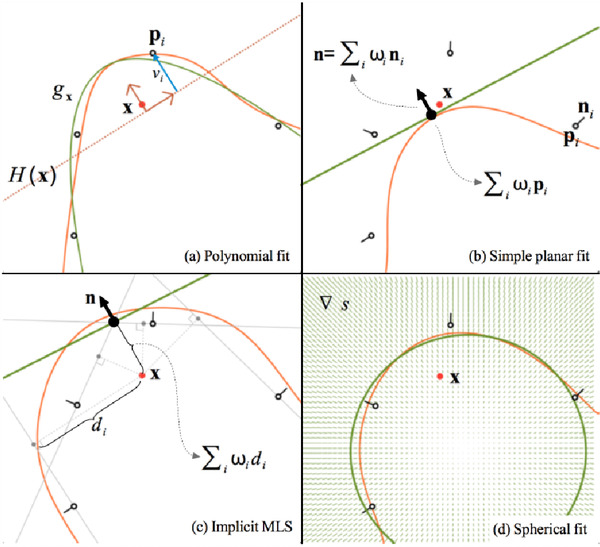
\includegraphics[width=13cm]{img/MLS.jpg}
  \caption{Ukážka princípu pre viacero variantov MLS v 2D. Miestne aproximácie vypočítané pre hodnotiaci bod $x$ sú znázornené zelenou farbou. Oranžové krivky zodpovedajú rekonštruovaným izo-kontúram. \cite{MLS_survey}} 
  \label{fig:MLS}
\end{figure} 

\subsubsection{MPU}
\noindent \acrshort{mpu} (Multi-level partition of unity) je metóda, ktorá bola špecificky vytvorená na rýchlu a presnú rekonštrukciu povrchu s veľkého súboru orientovaných bodov (body, ktoré obsahujú jednotkové normály). Názov metódy vyplýva zo podstaty fungovania \acrshort{mpu}, a to že sa skladá zo viacerých vážených funkcií, ktoré sa spočítavajú do jedna pre všetky body v doméne. Táto metóda ponúka adaptívny chybovo kontrolovaný odhad funkcie vzdialenosti od povrchu, čo znamená, že odhad je presný v blízkosti povrchu a hrubý ďaleko od povrchu. \cite{MPU_orig}
\newline\indent Pre vytvorenie implicitnej reprezentácie povrchu sa najprv všetky body rozdelia pomocou oktálového stromu. V každej bunke stromu sa vytvorí po častiach kvadratická funkcia (lokálna tvarová funkcia), ktorá sa snaží napasovať na body v bunke. Hodnota týchto funkcií nadobúda hodnotu 0 v blízkosti bodov, pozitívnu hodnotu vo vnútri a negatívnu (vonku) ďaleko od bodov. V prípade, že dosiahnutá presnosť je stále malá, bunka v oktálovom strome sa znovu rozdelí a celý proces sa opakuje, až dokým nie je dosiahnutá požadovaná presnosť (viď. Obr. \ref{fig:MPU}). Na záver v miestach, kde sa stretávajú hranice buniek, sú tvarovacie funkcie spojené dokopy na základe váh z funkcií rozdelenia jednoty (z ang. partition of unity functions). \cite{MPU_orig}
\begin{figure}[!htbp]
  \centering
  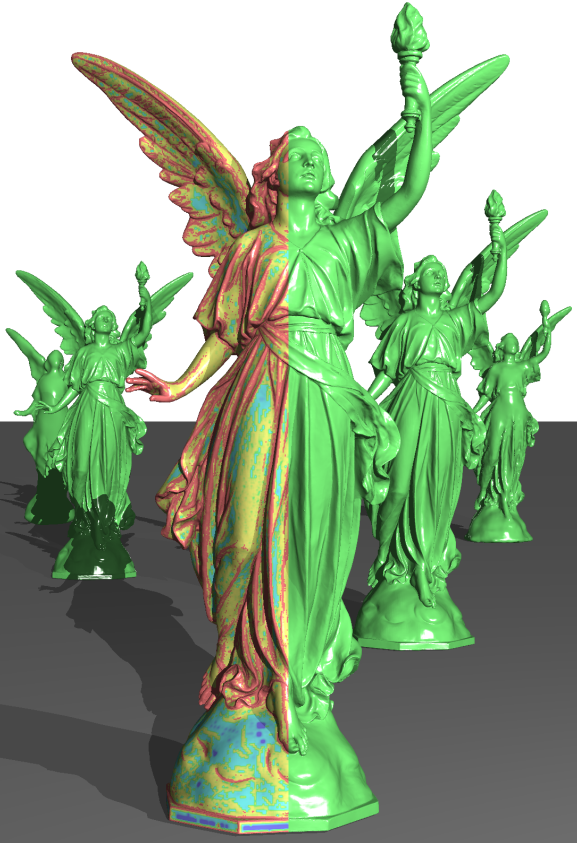
\includegraphics[width=8.5cm, height=10.5cm]{img/MPU_img.png}
  \caption{Ukážka rekonštrukcie pomocou \acrshort{mpu} implicit. Ľavá časť modelu je ofarbená podľa hĺbky rozdelenia, s tým že stúpa od modrej až po červenú. Modely v pozadí sú rekonštruované so stúpajúcou chybou v odhade. \cite{MPU_orig}} 
  \label{fig:MPU}
\end{figure} 

\subsection{Metódy pre zjednodušenie povrchu}
\noindent V mnohých prípadoch sa po rekonštrukcií povrchu z mračien bodov stretávame s tým, že povrch daného modelu obsahuje zbytočne veľa polygónov, pričom by ho bolo možné vyjadriť menším počtom a zároveň zachovať celkový tvar. V tejto podkapitole sa preto budeme zaoberať metódami, ktoré sa zameriavajú na zjednodušenie topológie povrchu, pričom ich delíme na lokálne a globálne metódy.  

\subsubsection{Lokálne metódy} \label{sec:decimation}
\noindent Lokálne metódy sú oproti globálnym bežnejšie, a preto sa budeme zaoberať hlavne nimi. Tieto metódy pristupujú k zjednodušovaniu iteratívnou aplikáciou lokálneho operátora na malú sadu bodov, čím vytvoria povrch s menším počtom prvkov. Využívajú chybové alebo nákladové (z ang. cost) funkcie, ktoré usmerňujú proces zjednodušovania, a taktiež ponúkajú presnú kontrolu výsledných atribútov povrchu (počet polygónov, hranice chýb pre vrcholy). \cite{mesh_simplification}
\begin{enumerate}
    \item\textbf{Decimácia vrcholov (z ang. Vertex decimation)} - Tento prístup pracuje s jedným vrcholom, ktorý sa vymaže a následne sa snaží zaplátať vytvorenú dieru na základe klasifikačnej schémy o susedstve. Výber vrcholu, ktorý bude vymazaný, je spojený so vzdialenosťou od roviny, ktorá je aproximovaná pomocou spriemerovania normál, ťažísk a plôch okolitých trojuholníkov. Vzdialenosť vrcholu od tejto roviny slúži, ako miera chyby pre jeho odstránenie, pričom vrcholy ležiace na hladkých častiach sú uprednostňované pred tými, ktoré opisujú ostré zmeny (detaily). \cite{mesh_simplification}
    \begin{figure}[!htbp]
      \centering
      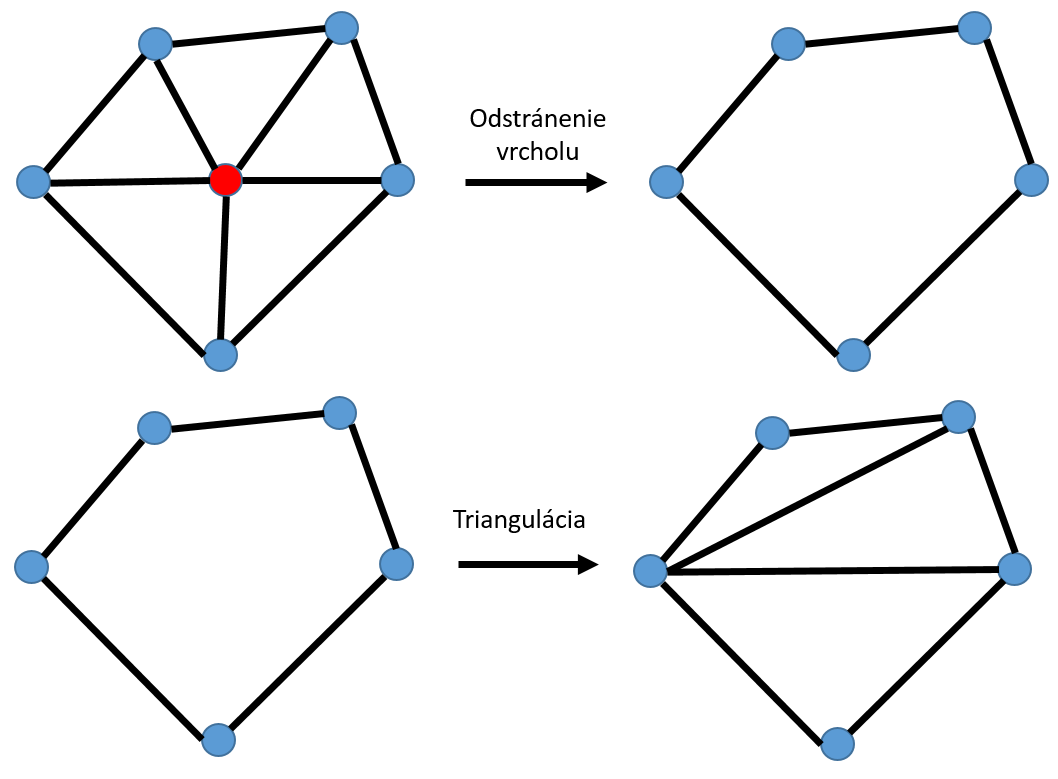
\includegraphics[width=12cm, height=8.5cm]{img/vertex_decim.png}
      \caption{Ukážka decimácie vrcholu v 2D} 
      \label{fig:vertex_decim}
    \end{figure} 
    \item\textbf{Kolaps strán (z ang. Edge collapse)} - V tejto metóde pracujeme s dvoma vrcholmi naraz, pričom ich výber môže byť vykonávaný ako v predošlej metóde. Táto metóda funguje na základe odstraňovania strán medzi vybranými vrcholmi, a teda zlučuje ich do jedného, pričom vždy ostarni dva trojuholníky. Ukázalo sa, že výber pozície nového vrcholu nie je až tak jasný, nakoľko uloženie do stredu medzi pôvodnými vrcholmi nie je optimálne. Vyvinulo sa preto niekoľko prístupov, ktoré rozhodujú o novom uložení a medzi najpopulárnejšie patrí prístup na základe kvadratickej chyby, ktorý je založený na umocnenej vzdialenosti vrcholov od aproximovanej roviny okolitých trojuholníkov. Tento prístup nájde optimálnu polohu nového vrcholu, tak aby sa zachovali aj ostré zmeny v povrchu.
    \begin{figure}[!htbp]
      \centering
      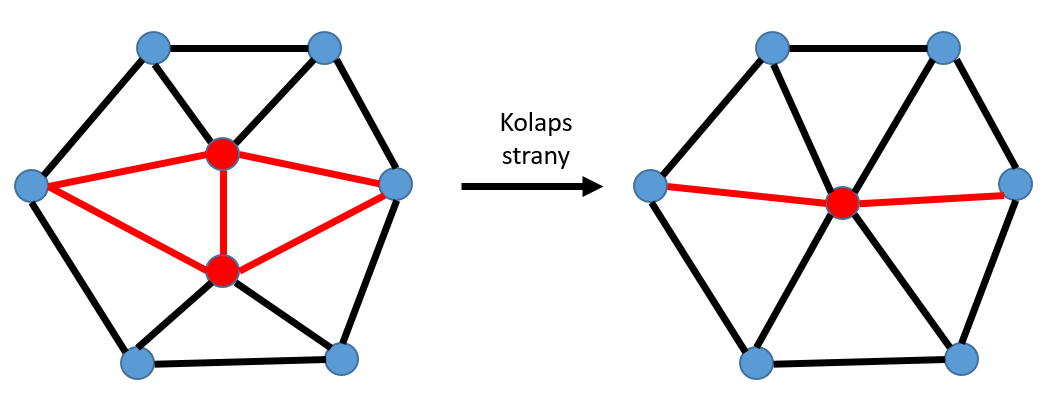
\includegraphics[width=12 cm]{img/edge_collapse.png}
      \caption{Ukážka kolapsu strany v 2D} 
      \label{fig:Edge_collapse}
    \end{figure} 
\end{enumerate}

\subsubsection{Globálne metódy}
\noindent Ako to už vyplýva z mena, globálne metódy pristupujú ku spracovaniu povrchu ako celku a na rozdiel od lokálnych metód, ktoré využívajú iteratíve procesy, globálne metódy analyzujú celý povrch naraz, aby dosiahli jeho zjednodušenie.
\begin{enumerate}
    \item\textbf{Zhlukovanie vrcholov (z ang. Vertex clustering)} - Táto metóda je založená na priradení váhy každému vrcholu, na základe jeho dôležitosti. Pre vrcholy susedné ku veľkým trojuholníkom a vrcholy v zakrivených oblastiach, je priradená väčšia váha, ako pre vrcholy v hladkých oblastiach a vedľa malých trojuholníkov. Celý priestor v ktorom sa povrch nachádza sa rozdelí pomocou voxelovej mriežky. Na záver sa všetky vrcholy v danej bunke mriežky zoskupia do vrcholu s najväčšou váhou, čím sa zníži celkový počet vrcholov. Táto metóda je výpočtovo veľmi efektívna, jej presnosť sa dá upravovať pomocou rozlíšenia voxelovej mriežky, ale taktiež vie zmeniť topológiu povrchu nepredvídateľným spôsobom. \cite{mesh_simplification}
\end{enumerate}

\newpage\vfill
\begin{figure}[ht]
  \centering
  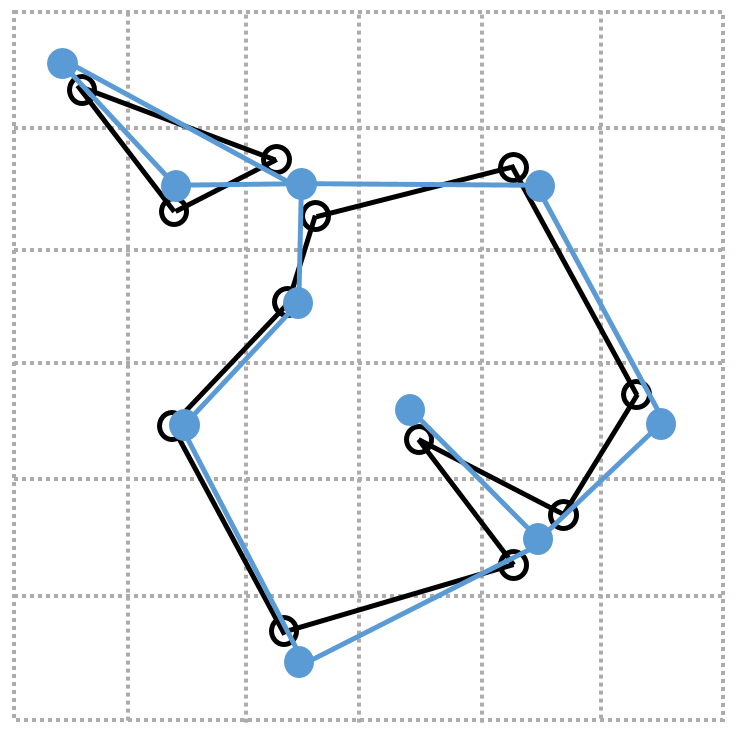
\includegraphics[width=10cm]{img/vertex_clustering.png}
  \caption{Ukážka zhlukovania vrcholov v 2D. Originálne vrcholy (čierne), po úprave (modré), pre viditeľnosť posunuté od stredu mriežky} 
  \label{fig:verte_cluster}
\end{figure} 
\vfill\clearpage

\section{Špecifikácia cieľov}
\noindent Po úspešnom zhrnutí rôznych prístupov pre spracovanie mračien bodov a rekonštrukciu povrchu v predošlých kapitolách, môžeme prejsť na návrh nášho riešenia. Navrhovaný algoritmus využije skôr spomínané metódy na predspracovanie mračna bodov, aby potom následná rekonštrukcia povrchu dosahovala lepšie výsledky, zatiaľ čo sa pokúsime o zníženie celkovej pamäťovej náročností na uloženie modelov. 
\newline\indent Tento proces môžeme rozdeliť do následujúcich bodov:
\begin{enumerate}
    \item Odstránenie odľahlých bodov
    \item Separácia bodov zeme a objektov
    \item Zhlukovanie bodov objektov do supervoxelov
    \item Segmentácia objektov
    \item Podvzorkovanie mračna bodov
    \item Rekonštrukcia povrchu
    \item Textúrovanie povrchu
\end{enumerate}

\section{Použité súbory dát}
\noindent Pred samotnou implementáciou navrhnutého riešenia si v krátkosti predstavíme mračná bodov, s ktorými budeme pracovať. Pre účely tejto práce nám bolo poskytnutých päť rozdielnych mračien bodov, pričom dve boli použité na vývoj a testovanie, a zvyšné boli použité na validáciu a overenie riešenia.
\newline\indent Pre získanie poskytnutých mračien bodov boli použité dva rozdielne \acrshort{lidar}-y. Mračno bodov mestskej časti s bytovkami (Obr. \ref{fig:SD1}) a mračno bodov mestskej časti s kruhovým odjazdom (Obr. \ref{fig:SD2}) boli namerané pomocou Optech CL-360 \acrshort{lidar}-u, zatiaľ čo mračno bodov parkoviska pri obchodoch (Obr. \ref{fig:SD3}), mračno bodov ulice so trolejbusovou zastávkou (Obr. \ref{fig:SD4}) a mračno bodov dedinskej časti (Obr. \ref{fig:SD5}) boli namerané pomocou Hesai XT-32 \acrshort{lidar}-u. V prípade prvých štyroch súborov dát bol \acrshort{lidar} pripevnený na streche auta, zatiaľ čo v posledom bol pripevnený na dronovi a dáta boli získane zo vzduchu.
\newline\indent  Pre jednoduchosť sa budú po zvyšok práce jednotlivé mračná bodov označovať, ako $SDx$, kde x je číslo súboru dát.

\begin{figure}[!htbp]
  \centering
  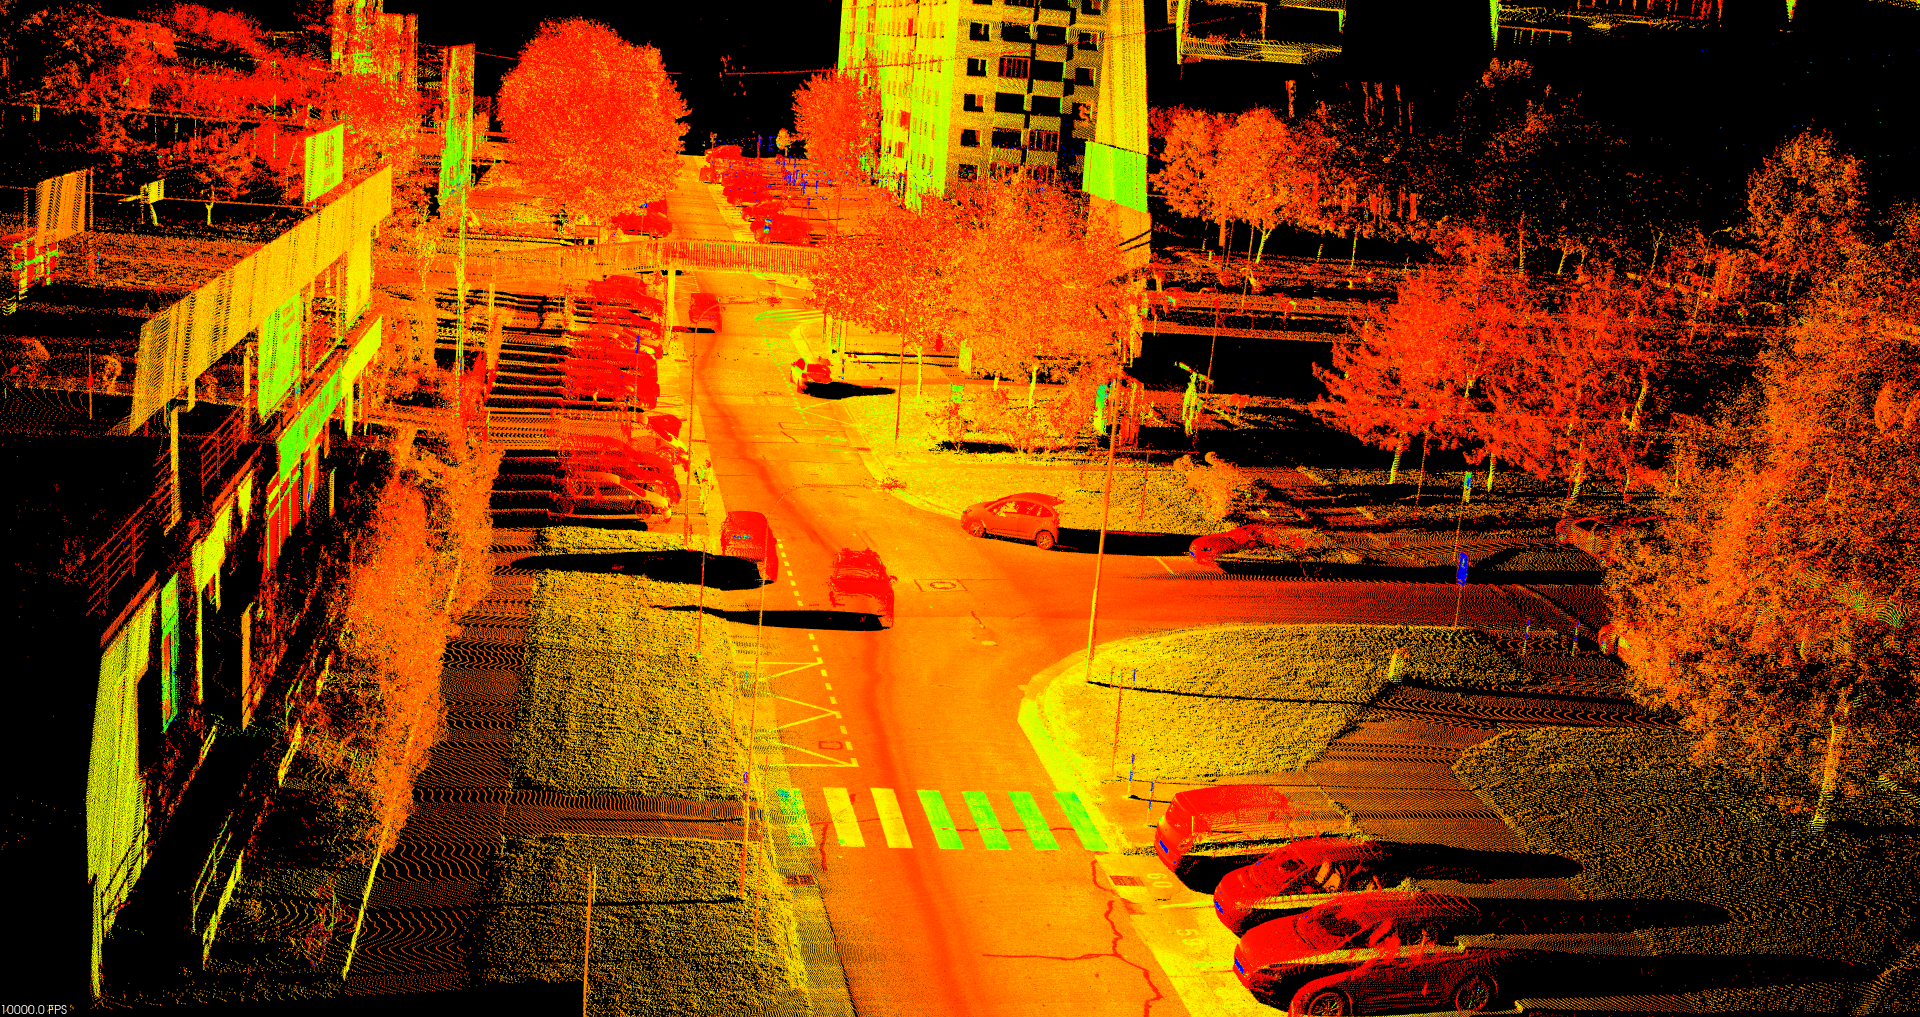
\includegraphics[width=16cm, height=10cm]{img/SD1_example.png}
  \caption{Mračno bodov mestskej časti s bytovkami - $SD1$ (Optech CL-360)} 
  \label{fig:SD1}
\end{figure} 

\begin{figure}[!htbp]
  \centering
  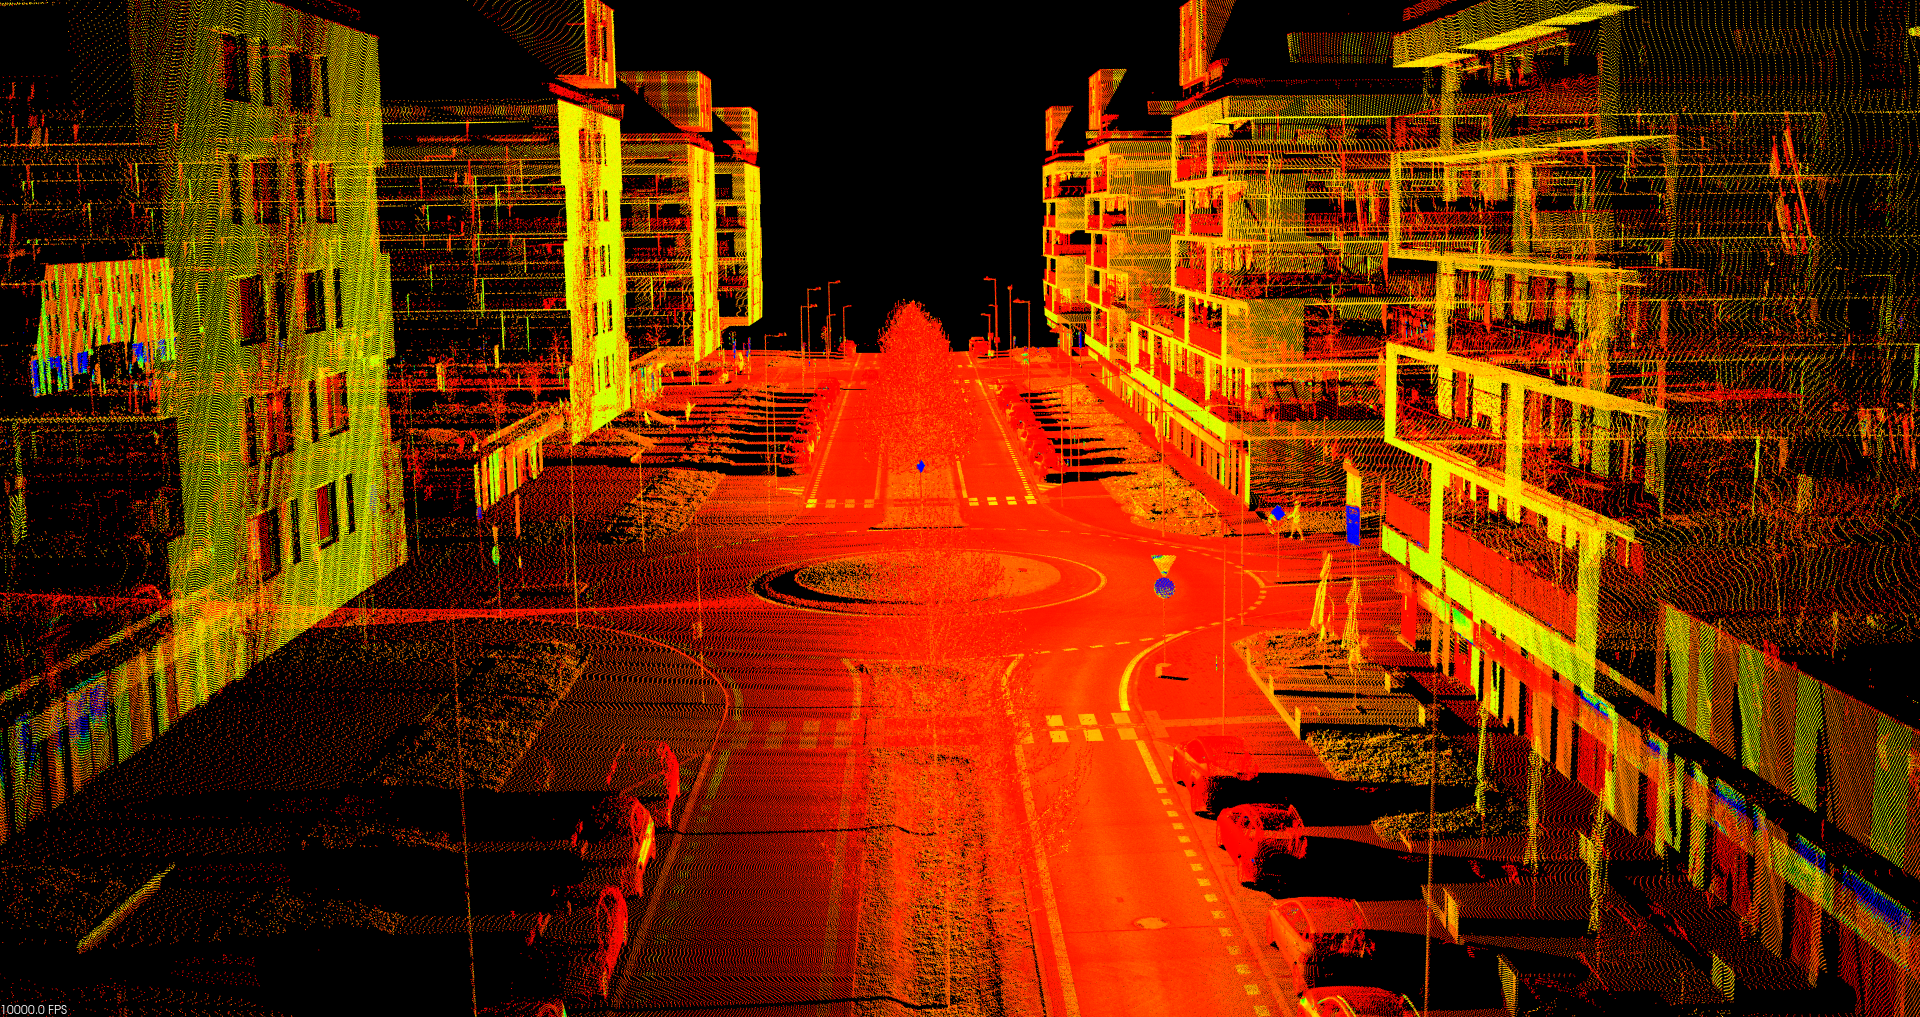
\includegraphics[width=16cm, height=10cm]{img/SD2_example.png}
  \caption{Mračno bodov mestskej časti s kruhovým odjazdom - $SD2$ (Optech CL-360)} 
  \label{fig:SD2}
\end{figure} 

\begin{figure}[!htbp]
  \centering
  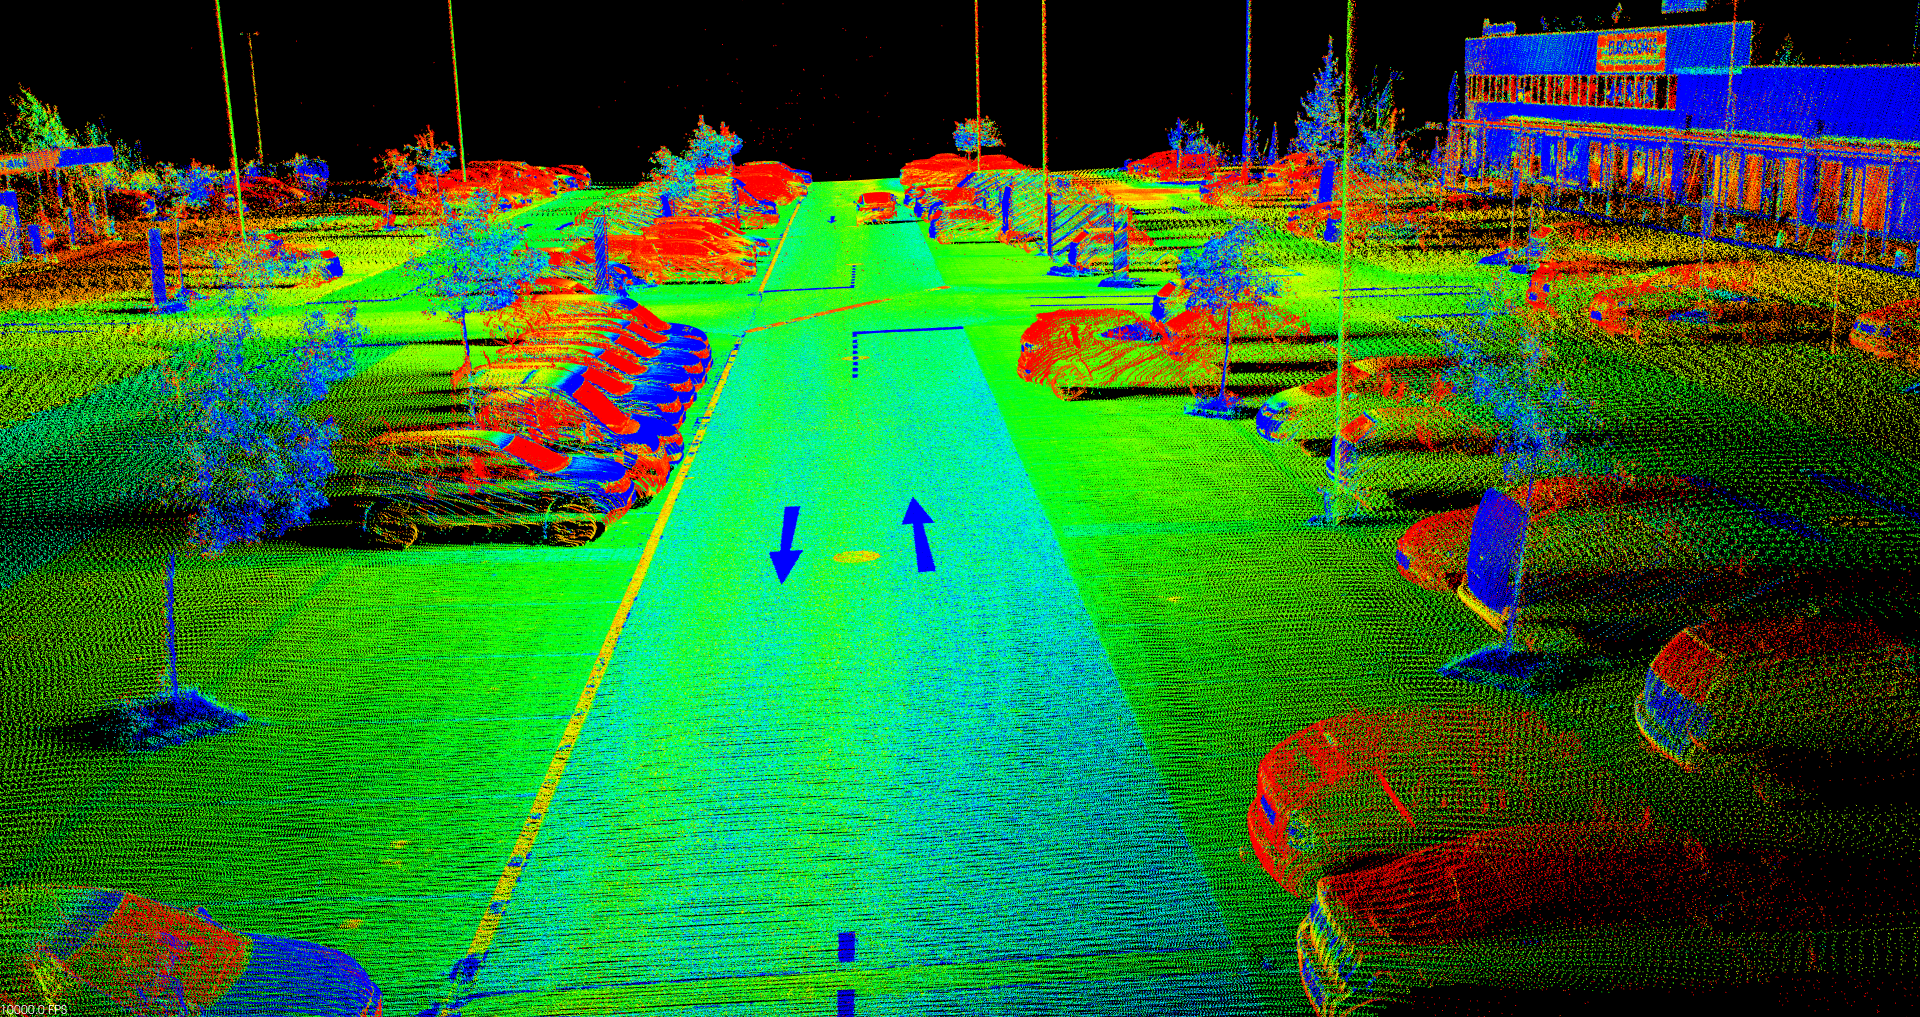
\includegraphics[width=16cm, height=10cm]{img/SD3_example.png}
  \caption{Mračno bodov parkoviska pri obchodoch - $SD3$ (Hesai XT-32)} 
  \label{fig:SD3}
\end{figure} 

\begin{figure}[!htbp]
  \centering
  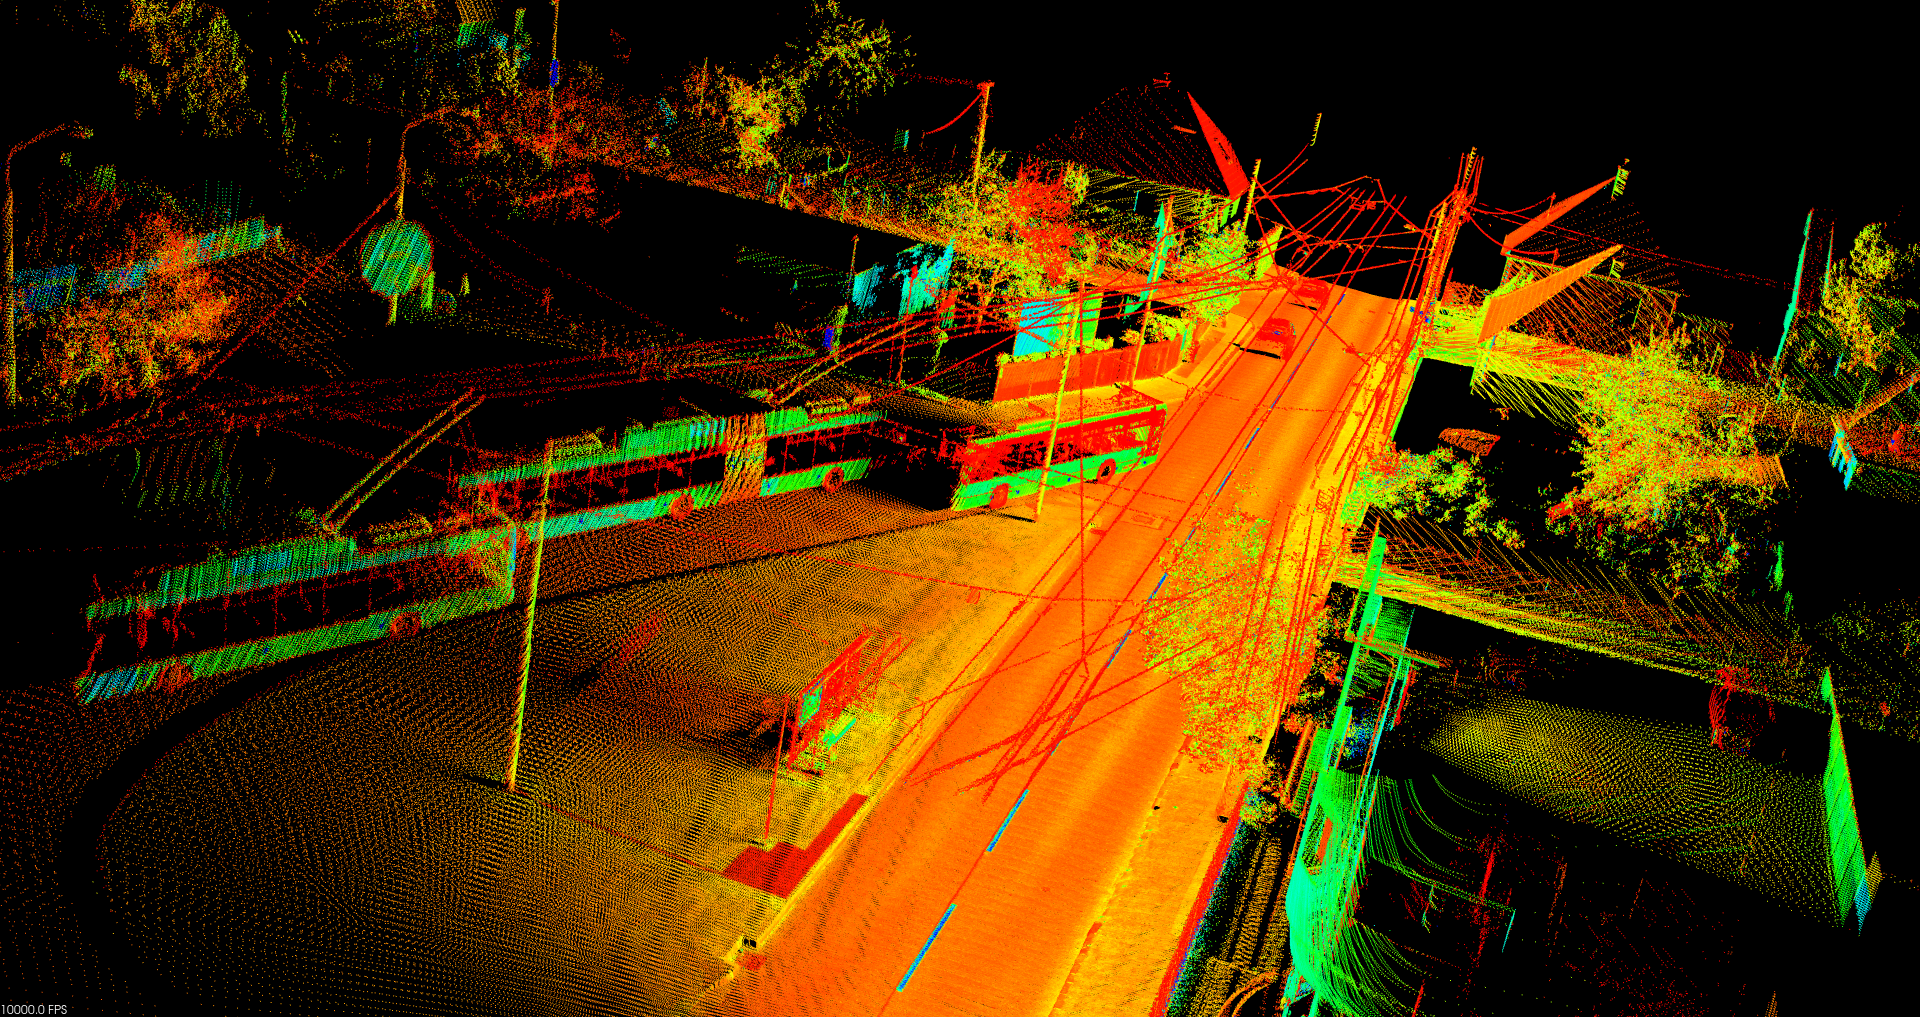
\includegraphics[width=16cm, height=10cm]{img/SD4_example.png}
  \caption{Mračno bodov ulice so trolejbusovou zastávkou - $SD4$ (Hesai XT-32)} 
  \label{fig:SD4}
\end{figure} 

\begin{figure}[!htbp]
  \centering
  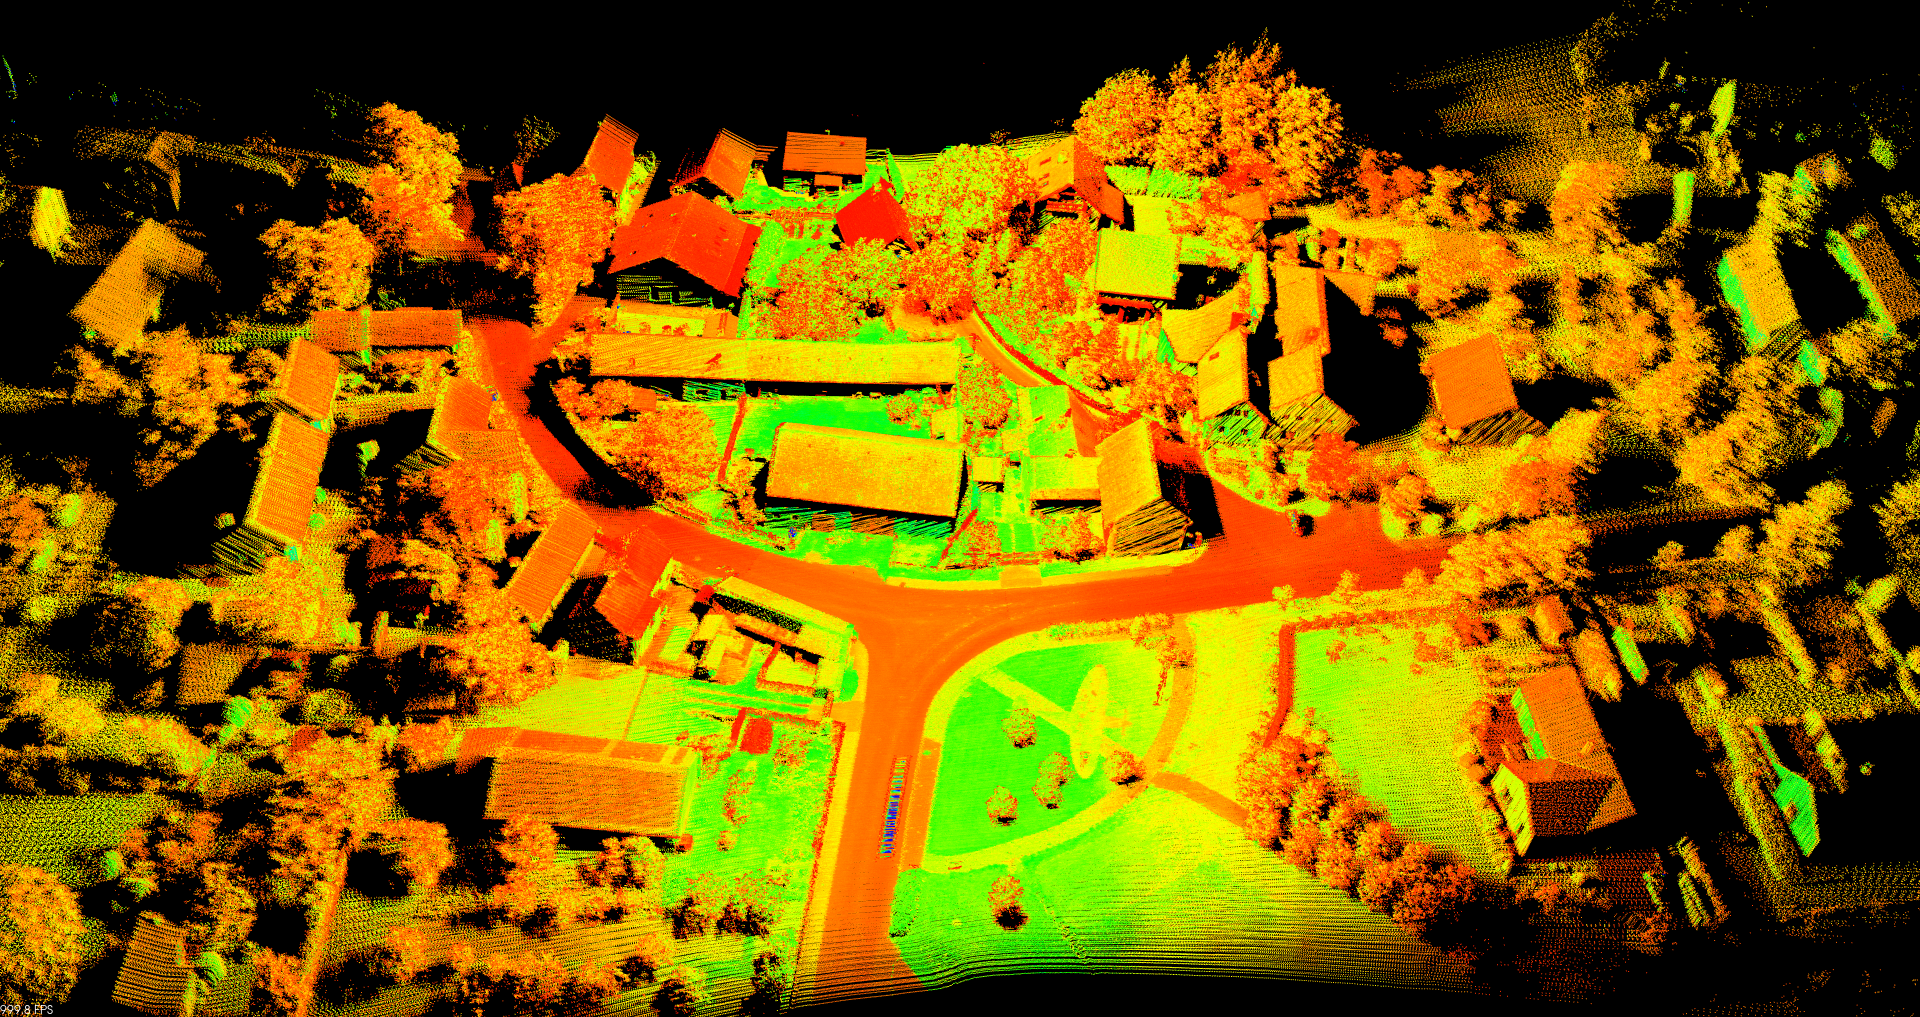
\includegraphics[width=16cm, height=10cm]{img/SD5_example.png}
  \caption{Mračno bodov dedinskej časti - $SD5$ (Hesai XT-32)} 
  \label{fig:SD5}
\end{figure} 

\section{Realizácia riešenia}
\noindent V tejto kapitole sa budeme zaoberať konkrétnou implementáciou vyššie špecifikovaných cieľov. Na implementáciu budeme používať programovací jazyk C++ v prostredí Visual Studio, pričom sa hlavne zameriame na využitie existujúcich implementácií algoritmov z \acrshort{pcl} knižnice.

\subsection{Odstránenie odľahlých bodov}
\noindent Ako už bolo uvedené v úvodnej kapitole, mračná bodov často obsahujú body, ktoré nereprezentujú reálny povrch objektov a nazývame ich odľahlé. Tieto body vznikajú z rôznych dôvodov, ako sú šum v systéme snímača, prekrytie snímača, lesklé alebo priehľadné povrchy objektov a mnoho ďalších. Odfiltrovanie týchto bodov je dôležitým krokom pri spracovaní mračien bodov, nakoľko ich odstránením nie len znížime celkový počet bodov, ale aj zabezpečíme, že nasledovné kroky budú mať vyššiu úspešnosť, či už ide o segmentáciu alebo samotnú rekonštrukciu povrchu. 
\newline\indent Pre samotné odstránenie odľahlých bodov nám \acrshort{pcl} knižnica ponúka dve rýchle a efektívne metódy, \acrshort{ror} (Radial outlier removal) a \acrshort{sor} (Statistical outlier removal). Prvá s týchto metód nám ponúka odstránenie bodov, ktoré nemajú minimálny počet susedov v definovanom rádiuse. Táto metóda je ale parametricky závislá od hustoty mračna bodov a pre rozdielne súbory dát nefunguje rovnako, a preto sme sa rozhodli, že budeme pokračovať so \acrshort{sor} metódou. Táto metóda počíta so priemernou vzdialenosťou každého bodu a jeho K najbližších susedov, na základe čoho vyhodnocuje, ktoré body sú odľahlé (presnejšie vysvetlené v kapitole \ref{section::sor}). 
\newline\indent Metóda nám ponúka nastavenie počtu najbližších susedov a násobiteľ prahu štandardnej odchýlky. Tieto dva parametre nám umožňujú nastavenie agresívnosti filtru a po vyskúšaní viacerých kombinácií, sme dospeli ku hodnotám:
\begin{itemize}
    \setlength\itemsep{0.2em}
    \item Počet najbližších susedov (z ktorých sa počíta priemer) = 20
    \item Násobiteľ prahu štandardnej odchýlky = 2,0
\end{itemize}
pre ktoré sme dosiahli dobrý pomer odstránenia nepotrebných (riedkych) bodov a zachovania podstatných bodov. Ukážku dosiahnutých výsledkov môžeme vidieť na Obr. \ref{fig:outlier}.

\newpage\vfill
\begin{figure}[ht]
  \centering
  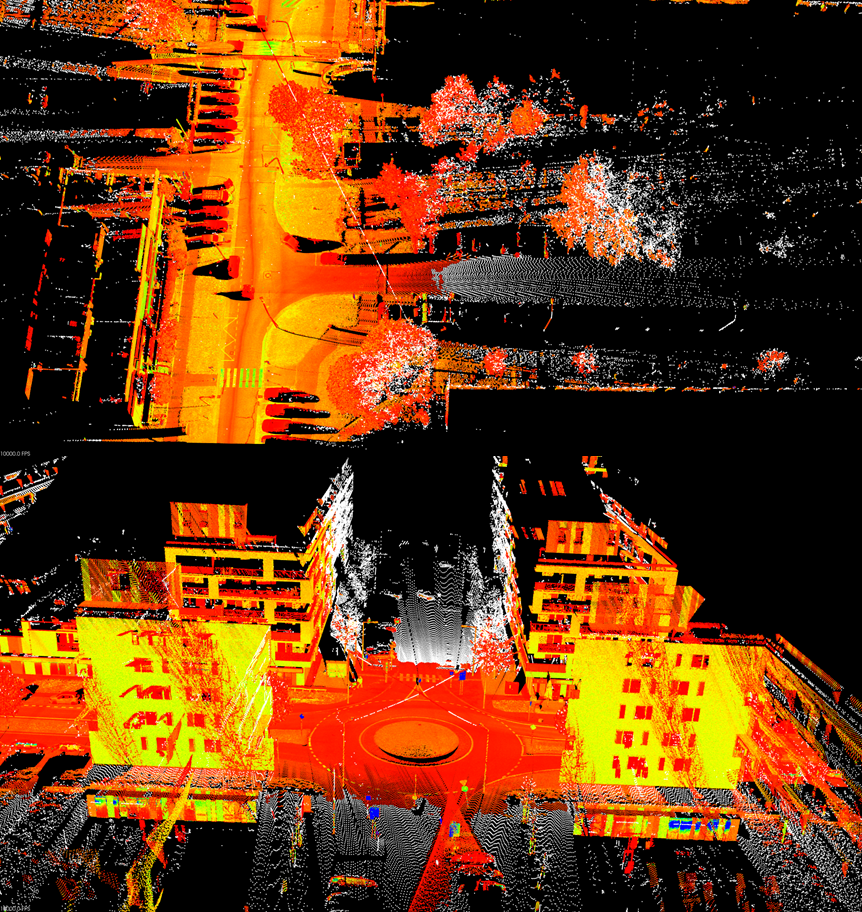
\includegraphics[width=16cm, height=19cm]{img/outlier_removal.png}
  \caption{Výsledné mračná bodov (pôvodná farba) po odstránení odľahlých bodov (biele farba) pomocou \acrshort{sor} metódy ($SD1$ hore, $SD2$ dole)} 
  \label{fig:outlier}
\end{figure} 
\vfill\clearpage

\begin{table}
    \begin{center}
        \begin{tabular}{|c || c | c | c| c|} 
         \hline
         &  \thead{Pôvodný počet \\ bodov} &
            \thead{Nový počet \\ bodov} &
            \thead{Zmenšenie mračna \\ bodov [\%]} &
            \thead{Potrebná \\ pamäť [MB]} \\ [0.5ex] 
         \hline\hline
         \textbf{SD1} & 15 667 351 & 15 477 814 & 1,21 & 221,70 \\ 
         \hline
         \textbf{SD2} & 5 297 511 & 5 144 894 & 2,89 & 176,20 \\
         \hline
         \textbf{SD3} &  9 924 233 & 9 797 094 & 1,29 & 140,20 \\
         \hline
         \textbf{SD4} & 5 462 647 & 5 344 810 & 2,16 & 76,40 \\
         \hline
         \textbf{SD5} & 7 544 836 & 7 297 335 & 3,28 & 104,70 \\
         \hline
        \end{tabular}
    \caption{Porovnanie veľkosti pôvodných a filtrovaných mračien bodov, pre jednotlivé súbory dát}
    \end{center}
\end{table}

\subsection{Separácia bodov zeme a objektov}
\noindent Po odfiltrovaní odľahlých bodov je ďalším hlavným cieľom segmentovať mračno bodov na jednotlivé objekty. Pred samotnou segmentáciou je vhodné separovať body zeme (terénu) od bodov jednotlivých objektov, nakoľko v drvivej väčšine prípadov, sú tieto body navzájom spojené iba so samotnou zemou.
\newline\indent Pre tento účel využijeme progresívny morfologický filter. Princíp tohto filtra spočíva vo využití matematickej operácie otvárania (kombinácia erózie a následnej dilatácie), ktorá sa aplikuje na body v tzv. “okne”. Ak je toto okno väčšie ako objekt reprezentovaný bodmi vo vnútri, objekt je odstránení, zatiaľ čo väčšie objekty sú zachované. Táto metóda začína vytvorením mriežky s počiatočnou veľkosťou okna, pričom odstraňuje menšie objekty. Postupným zväčšovaním tohto okna odstraňuje stále väčšie objekty, až kým nedosiahne maximálnu veľkosť okna, kedy by mali byť zachované len body zeme. \cite{morph_filter}
\newline\indent V našej práci využijeme implementáciu z \acrshort{pcl} knižnice, konkrétne využijeme jeho aproximáciu, keďže jeho plná verzia je výpočtovo a časovo veľmi náročná. Metóda ponúka viacero nastaviteľných parametrov, pričom pre následujúcu konfiguráciu sme dosiahli najlepšie výsledky (viď. Obr. \ref{fig:ground_sep}). 

\begin{itemize}
    \setlength\itemsep{0.2em}
    \item Maximálna veľkosť okna = 18
    \item Veľkosť bunky = 0,1
    \item Sklon = 2,85
    \item Počiatočná vzdialenosť (nad parametrizovaným povrchom) = 0,1
    \item Maximálna vzdialenosť (nad parametrizovaným povrchom) = 2,5
\end{itemize}

\newpage\vfill
\begin{figure}[ht]
  \centering
  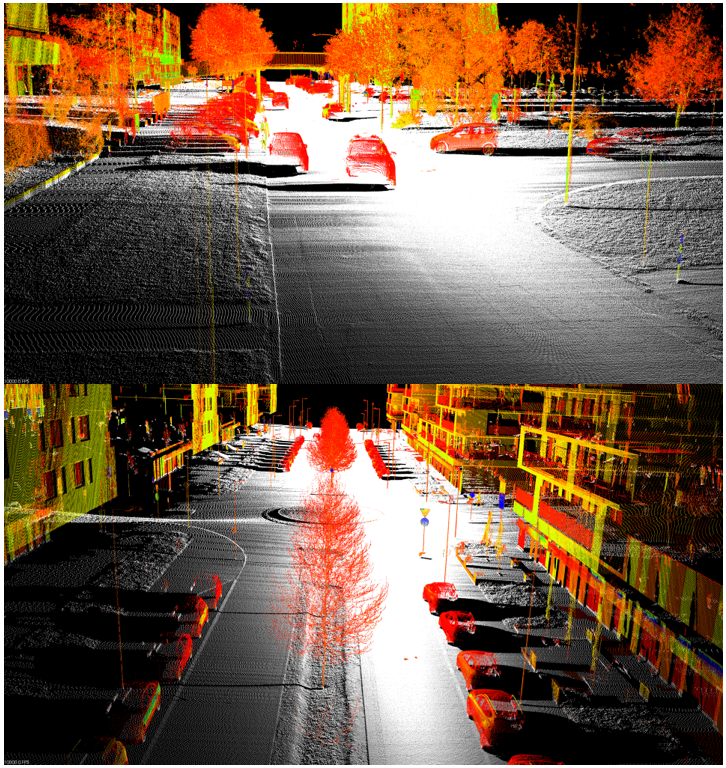
\includegraphics[width=16cm, height=19cm]{img/morph_filter.png}
  \caption{Mračná bodov objektov (pôvodná farba) po separácií bodov zeme (biele farba) pomocou aproximácie morfologického filtra ($SD1$ hore, $SD2$ dole)} 
  \label{fig:ground_sep}
\end{figure} 
\vfill\clearpage

\begin{table}
    \begin{center}
        \begin{tabular}{|c || c | c | c|} 
         \hline
          & \textbf{Počet bodov zeme} & \textbf{Počet bodov objektov} & \textbf{Pomer bodov zeme a objektov[\%]} \\ [0.5ex] 
         \hline\hline
         \textbf{SD1} & 8 455 280 & 7 022 534 & 54,63 - 45,37 \\ 
         \hline
         \textbf{SD2} & 3 075 670 & 2 069 224 & 59,78 - 40,22 \\
         \hline
         \textbf{SD3} &  5 260 628 & 4 536 466 & 53,70 - 46,30 \\
         \hline
         \textbf{SD4} & 3 321 577 & 2 023 233 & 62,15 - 37,85 \\
         \hline
         \textbf{SD5} & 3 206 050 & 4 091 285 & 43,93 - 56,07 \\ 
         \hline
        \end{tabular}
    \caption{Porovnanie pomeru bodov zeme a objektov, pre jednotlivé súbory dát}
    \label{table::ground_separation}
    \end{center}
\end{table}

\subsection{Zhlukovanie bodov objektov do supervoxelov}
\noindent Pre účely použitia nasledujúcej segmentačnej metódy, je potrebne mračno bodov zoskupiť do tzv. supervoxelov, ktoré predstavujú významovo väčšie celky, ktoré majú podobné vlastnosti, zatiaľ čo sa snažia nepresahovať hranice objektov. Tieto zhluky taktiež predstavujú vyššiu úroveň reprezentácie mračna bodov, čím redukujú výpočtovú náročnosť ďalších procesov, zatiaľ čo uchovávajú dôležité štrukturálne informácie. 
\newline\indent Zoskupenie mračna bodov vykonáme pomocou \acrshort{pcl} knižnice, ktorá obsahuje triedu Supervoxel Clustering. Táto trieda vykonáva zhlukovanie využitím \acrshort{vccs} (Voxel Cloud Connectivity Segmentation), čo je nová metóda, ktorá využíva rastový variant k-means zhlukovania, pričom body označuje priamo do voxelov štruktúry oktálového stromu. Pomocou oktálového stromu efektívne uchováva graf súslednosti 26 susedov (spojený hranou, tvárou alebo vrcholom), pričom tento graf je vo veľkej miere použitý pre rast regiónov zhlukov, ako aj pre uchovanie súslednosti výsledných supervoxelov. Rast supervoxelov je riadený normalizovanými priestorovými, farebnými a normálovými vzdialenosťami, pričom prvá meria priestorový rozsah, druhá meria rozdiel farby v RGB priestore a posledná meria uhol medzi normálami povrchu. \cite{supervoxelClustering}
\newline\indent Trieda Super-voxel Clustering ponúkala nastavenie piatich parametrov, pričom hodnota rozlíšenia voxelov, rozlíšenia počiatočných bodov a dôležitosť normál hrala najvýznamnejšiu úlohu. Výsledná konfigurácia parametrov je nasledovná:

\begin{itemize}
    \setlength\itemsep{0.2em}
    \item Rozlíšenie voxelov = 0,1
    \item Rozlíšenie počiatočných bodov (z ang. seed)  = 1,0
    \item Dôležitosť normál = 1,0
    \item Dôležitosť farby = 0,2
    \item Priestorová dôležitosť = 0,2
\end{itemize}

\newpage\vfill
\begin{figure}[ht]
  \centering
  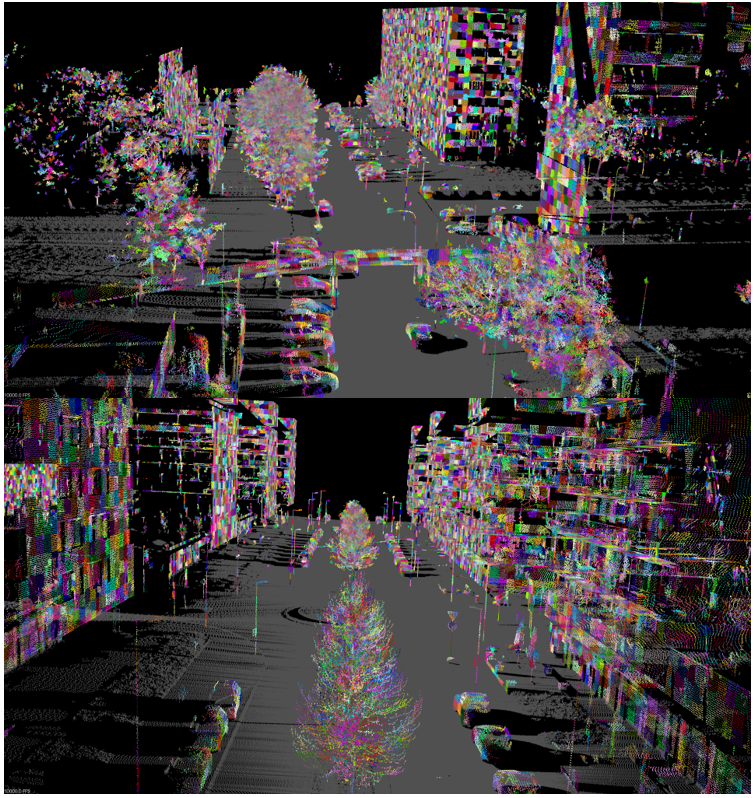
\includegraphics[width=16cm, height=19cm]{img/supervoxel.png}
  \caption{Mračná bodov objektov zoskupené do supervoxelov rôznej farby ($SD1$ hore, $SD2$ dole)} 
  \label{fig:supervoxel}
\end{figure} 
\vfill\clearpage

\subsection{Segmentácia mračna bodov}
\noindent Výsledkom predošlých krokov je samotná segmentácia mračna bodov objektov. Táto segmentácia nám rozdelí body mračna na jednotlivé objekty, čo následne umožní individuálny prístup pri ďalších krokoch, ako sú podvzorkovanie alebo rekonštrukcia povrchu. Vďaka segmentácií budeme mať väčšiu kontrolu a dosiahneme lepšie výsledky.
\newline\indent Pre segmentáciu mračna bodov využijeme \acrshort{pcl} implementáciu \acrshort{cpc} (Constrained Planar Cuts) metódy. Táto metóda využíva graf súsledností vytvorený v predošlom kroku pomocou \acrshort{vccs}, na to aby získala informáciu o lokálnych konkávnostiach/konvexnostiach, pomocou čoho vytvára EEC (Euclidean Edge Cloud). Toto mračno hrán reprezentuje každý bod, ako hranu grafu súslednosti, pričom uchováva veľkosť hrany a jej smer (konvexný alebo konkávny). Na základe tejto reprezentácie, je možné využiť geometricky obmedzený deliaci model, pre nájdenie možných rezov. Pre určenie roviny rezu je použitý vážený \acrshort{ransac}, ktorý sa snaží maximalizovať hodnotiacu funkciu, pričom body s konkávnym smerom hrany sú uprednostňované pred tými so konvexnou. Mračno bodov je na základe tejto roviny rekurzívne rezané, až pokým nie sú dosiahnuté ukončovacie podmienky, čím získavame výsledné segmentované mračno bodov. \cite{CPCsegmentation}
\newline\indent Samotná \acrshort{pcl} implementácia ponúka viacero nastaviteľných parametrov, pričom rôzne konfigurácie majú svoje výhody a nevýhody. Výsledná konfigurácia vyzerá následovne:

\begin{itemize}
    \setlength\itemsep{0.1em}
    \item Prah tolerancie konkávnosti (uhol v stupňoch) = 15,0
    \item Maximálny počet rezov = 20
    \item Minimálna veľkosť rezaného segmentu = 300
    \item Minimálna veľkosť segmentu (menšie budu zlúčené) = 150
    \item Počet \acrshort{ransac} iterácií = 3000
    \item K-faktor (faktor pre rozšírenú kontrolu konvexnosti) = 0
    \item Minimálne rezné skóre (skóre na vykonanie rezu) = 0,3
    \item Prah hladkosti (kontrola hladkosti hrán) = 0,1
    \item Použitie kritéria rozumnosti (odstránenie oblastí s jedným spojením) = nie
    \item Použitie lokálnych obmedzení rezania = áno
    \item Použitie usmerneného rezania (kolmé rezanie na hranu) = nie
    \item Čisté rezanie (rezanie hrán so suprevoxelmi na opačných stranách roviny) = áno
\end{itemize}

\newpage\vfill
\begin{figure}[ht]
  \centering
  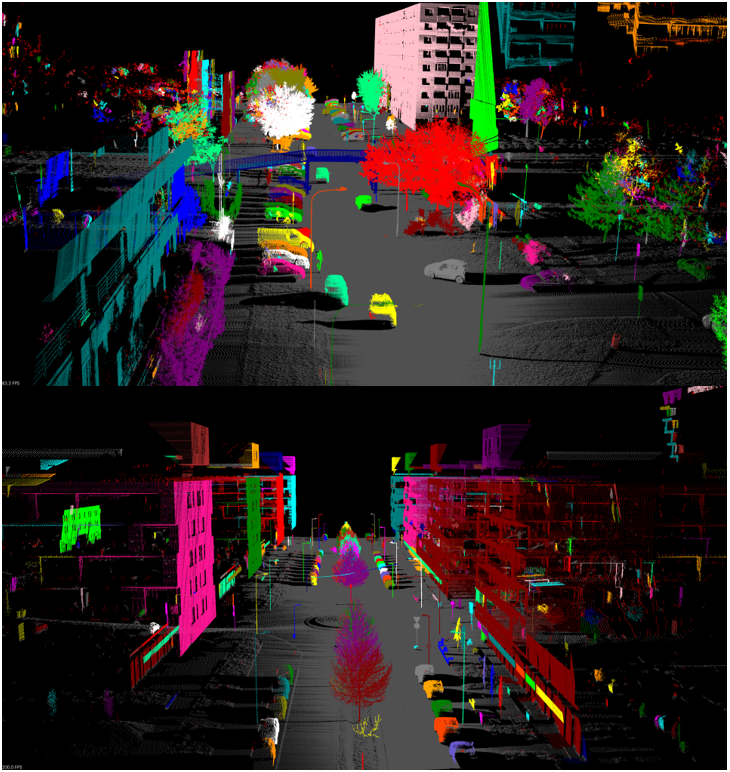
\includegraphics[width=16cm, height=19cm]{img/segmentation.png}
  \caption{Mračná bodov segmentované na jednotlivé objekty, označené rôznou farbou ($SD1$ hore, $SD2$ dole)} 
  \label{fig:cpc_seg}
\end{figure} 
\vfill\clearpage

\subsection{Podvzorkovanie mračna bodov}
\noindent Ďalším krokom pred samotnou rekonštrukciou povrchu je podvzorkovanie mračna bodov. Tento krok nám zníži celkový počet bodov, čo zabezpečí nie len zníženie pamäťovej náročnosti, ale aj zníženie výpočtového času pri rekonštrukcií povrchu. Pre tento účel budeme používať dve odlišné metódy, pričom budeme rozdielne pristupovať ku bodom zeme a ku bodom objektov.
\subsubsection{Podvzorkovanie bodov objektov}
\noindent Ako prvými sa budeme zaoberať bodmi objektov, ktoré obsahujú pomerne veľa detailov, ktoré chceme zachovať, a preto zvolíme adaptívny prístup podvzorkovania.
\newline\indent Pre tento účel využijeme \acrshort{don} (Difference of Normals), pomocou ktorého klasifikujeme jednotlivé body objektu podľa ich dôležitosti. Táto metóda je založená na odhade normál pomocou dvoch rôznych rádiusov, v ktorých vyhodnocuje body. Myšlienka je tá, že ak je odhad normál robený na rovnom povrchu, pre obidve rádiusy bude smer normály podobný, a tým pádom ich diferencia bude minimálna. Naopak ak je tento odhad robený na zakrivenom povrchu ich smer bude rozdielny, a tým pádom aj ich diferencia bude veľká (vid. Obr. \ref{fig:Don_principle}). Na základe veľkosti novej normály (0 - 1), ktorá vznikla diferenciou, vieme určiť úroveň zakrivenia povrchu v danom bode, a teda môžeme dané body klasifikovať podľa ich úrovne dôležitosti, pričom viac zakrivený povrch je dôležitejší.
\newline\indent Pre samotné podvzorkovanie využijeme voxelovú mriežku, ktorá rozdelí priestor bodov na rovnomerné voxely, pričom vždy zachová iba bod najbližší ku ťažisku voxelu. Pre rôzne triedy dôležitosti sme využili rôzne rozlíšenie voxelovej mriežky, ktoré prináleží dôležitosti danej triedy. Objekty sme rozdelili do štyroch tried a podvzorkovali sme ich pri nasledovnej konfigurácií parametrov:

\begin{itemize}
  \setlength\itemsep{0.2em}
  \item Rádiusy pre odhad normál (malý, veľký) = 0,03-0,07 ; 0,40
  \item Veľkosť diferencie normál (trieda 1-4) = (0-0,06) ; (0.06-0,10) ; (0,10-0,13) ; (0,13-1,0)
  \item Rozlíšenie voxelovej mriežky (trieda 1-4) = 0,13 ; 0,05 ; 0,02 ; 0,00 (bez podvzorkovania)
\end{itemize}

\begin{figure}[!htbp]
  \centering
  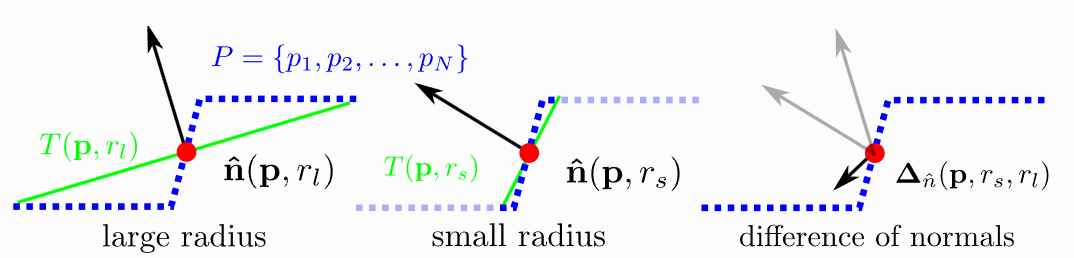
\includegraphics[width=15cm, height=3.3cm]{img/Don_principle.png}
  \caption{Ukážka princípu fungovania \acrshort{don} na zakrivenom povrchu \cite{DoN_segmentation}} 
  \label{fig:Don_principle}
\end{figure} 

\newpage\vfill
\begin{figure}[ht]
  \centering
  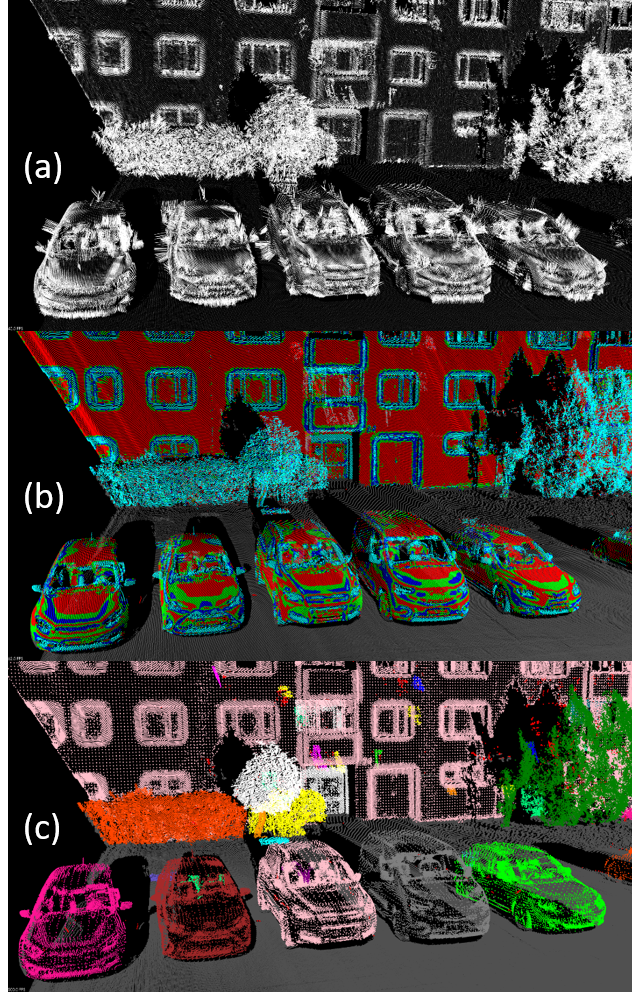
\includegraphics[width=15cm, height=21cm]{img/downsample_objects.png}
  \caption{(a) Mračno diferencií normál (b) Klasifikované mračno na základe dôležitosti bodov v vzostupnom poradí červené, zelené, modré a najdôležitejšie tyrkysové (c) Výsledné podvzorkované mračno bodov objektov ($SD1$)} 
  \label{fig:downsampling_objects}
\end{figure} 
\vfill\clearpage

\subsubsection{Podvzorkovanie bodov zeme}
\noindent Po podvzorkovaní bodom objektov ostávajú iba body zeme. Tieto body v drvivej väčšine neobsahujú toľko detailov ako body objektov, a preto na ich podvzorkovanie využijeme iba druhú časť predošlého postupu, a teda podvzorkujeme ich pomocou voxelovej mriežky s fixným rozlíšením, čo zabezpečí vysokú úroveň podvzorkovania.
\newline\indent Toto rozhodnutie sme urobili hlavne z dôvodu, že body zeme obsahujú hlavne rovinné plochy, ktoré majú medzi sebou pomerne hladký prechod. Ak by sme chceli využiť predošlí postup aj na body zeme, zbytočne by sme zvýšili ponechaný počet bodov, nakoľko oblasti s nízkou vegetáciou, ako je tráva, obsahujú pomerne nerovný povrch, pričom aj pri ponechaní viacerých bodov, sú zložité na dôveryhodnú rekonštrukciu povrchu. 
\newline\indent Konfigurácia pre podvzorkovanie bodov zeme je nasledovná:

\begin{itemize}
  \setlength\itemsep{0.2em}
  \item Rozlíšenie voxelovej mriežky = 0,20
\end{itemize}

\begin{figure}[!htbp]
  \centering
  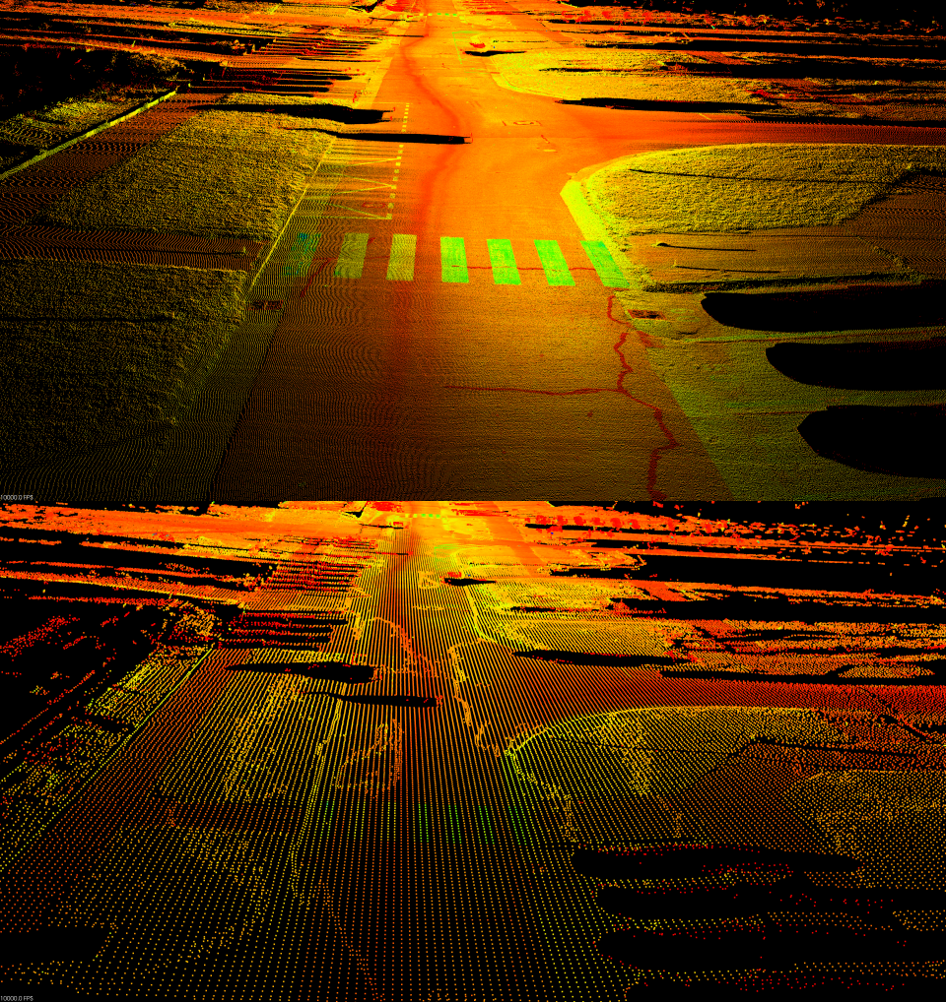
\includegraphics[width=15cm, height=13cm]{img/downsample_ground.png}
  \caption{Mračno bodov zeme pred (hore) a po (dole) podvzorkovaní. ($SD1$)} 
  \label{fig:downsample_ground}
\end{figure} 

\begin{table}
    \begin{center} % Center the table
        \begin{tabular}{|c || c | c | c | c | c| c|} 
         \hline
          & \thead{Nový \\ počet \\ bodov \\ zeme} &
            \thead{Nový \\ počet \\ bodov \\ objektov} &
            \thead{Zmenšenie \\ počtu \\ bodov \\ zeme [\%]} &
            \thead{Zmenšenie \\ počtu \\ bodov \\ objektov [\%]} &
            \thead{Celkové \\ zmenšenie \\ počtu \\ bodov [\%]} & 
            \thead{Celková \\ potrebná \\ pamäť [MB]} \\ [0.5ex]    
         \hline\hline
         \textbf{SD1} & 244 262  & 4 229 627 & 97,11 & 39,77 & 71,09 & 64,60  \\ 
         \hline
         \textbf{SD2} & 192 495  & 1 297 412 & 93,74 & 32,01 & 68,91 & 23,10 \\
         \hline
         \textbf{SD3} &  237 870  & 1 468 073 & 95,47 & 60,89 & 79,46 & 29,00 \\
         \hline
         \textbf{SD4} & 63 678  & 1 204 318 & 98,08 & 37,67 & 75,21 & 19,00 \\
         \hline
         \textbf{SD5} & 582 313  & 3 197 181 & 81,83 & 21,31 & 47,90 & 54,70 \\ 
         \hline
        \end{tabular}
    \caption{Porovnanie zmenšenia počtu bodov pred (viď. Tab. \ref{table::ground_separation}) a po podvzorkovaní mračien bodov}
    \label{table:subsampling}
    \end{center}
\end{table}

\subsection{Rekonštrukcia povrchu}
\noindent Predošlým predspracovaním dostávame podvzorkované mračno bodov, očistené od odľahlých bodov, ktoré je zároveň segmentované na jednotlivé objekty, vďaka čomu môžeme prejsť na samotnú rekonštrukciu povrchu. Prvým krokom pri rekonštrukcií povrchu bude výber použitej metódy, ktorá dosahuje najlepšie výsledky.  

\subsubsection{Výber metódy}
\noindent Pri výbere metódy na rekonštrukciu sa zameriame na metódy, ktoré ponúka \acrshort{pcl} knižnica, a to sú Poissonová rekonštrukcia, Marching cubes (Hoppe) a \acrshort{gpt} (Greedy projection trinagulation). Principiálne fungovanie prvých dvoch bolo bližšie vysvetlené v kapitolách \ref{sec:poisson}, \ref{sec:marching_cubes} a \acrshort{gpt} metódu si v krátkosti vysvetlíme teraz. 
\newline\indent Fungovanie tejto metódy je pomerne jednoduché a vieme ju rozdeliť do štyroch základných krokov. Prvým krokom je nájdenie lokálnych susedstiev pre každý bod, ktoré je zložené z $K$ najbližších susedov. Následne je vykonaný odhad normál každého referenčného bodu, pomocou čoho je vytvorená rovina, ktorá je kolmá na smer normály a všetky body zo susedstva sú projektované na túto rovinu. Na tejto rovine je použitý priestorovo rastúci algoritmus, ktorý sa z počiatočného trojuholníku rozrastá, až kým nie je skompletizovaný celý povrch, pričom dodržuje obmedzenia. Na záver sa projektovaná reprezentácia vráti do pôvodného 3D priestoru, čím dostávame výsledný povrch. \cite{GreedyTriangulation}
\newline\indent Pri výbere používanej metódy sa zameriame na hodnotiace faktory, ako sú dôveryhodnosť rekonštruovaného povrchu, časová náročnosť a výpočtová náročnosť (obmedzenia hardvéru). Na obrázku \ref{fig:mesh_compararison} môžeme vidieť dosiahnuté výsledky jednotlivých metód, ktoré boli upravené pre potreby porovnávania. Čo sa týka dôveryhodnosti najlepšie výsledky dosahuje Poissonová metóda, ktorá vytvára hladký vodotesný povrch, ktorý dobre zachytáva aj menšie detaily. Porovnateľne dobrá je aj \acrshort{gpt} metóda, ktorá je ale parametricky závislá od veľkosti a hustoty objektu, čo vedie ku nežiadaným dieram v povrchu. Posledná je Marching cubes metóda, ktorá vytvára kockovaný povrch, ktorý nie je prirodzený a vedie ku skresľovaniu výzoru objektu.
\newline\indent V prípade časovej a výpočtovej náročnosti bola najlepšia \acrshort{gpt} metóda, ktorá povrch ukážkového objektu zrekonštruovala najrýchlejšie (1,35s), pričom porovnateľne rýchla bola aj Poissonová rekonštrukcia (1,74s), ktorá ale následne potrebovala ďalšie úpravy. Najpomalšia bola Marching cubes (16,26s), ktorá ako jediná mála hardvérový problém a nebolo ju možné skúsiť na objektoch s väčším množstvom bodov. 
\newline\indent S predošlých výsledkov bolo rozhodnuté, že sa budeme pokračovať s Poissonovou metódou rekonštrukcie povrchu, nakoľko vizuálne dosahovala najlepšie výsledky a nie je parametricky závislá od hustoty mračna bodov. Metóda má ale svoje nedostatky, ktoré budú prebrané v ďalšej podkapitole. 

\begin{figure}[!htbp]
  \centering
  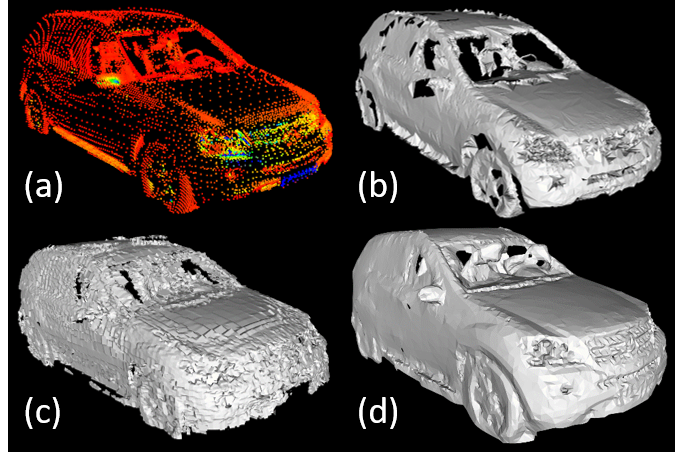
\includegraphics[width=16cm, height=11cm]{img/mesh_methods_compararison.png}
  \caption{Porovnanie rôznych metód rekonštrukcie povrchu na objekte auta - (a) Podvzorkované mračno bodov (b) \acrshort{gpt} (c) Marching cubes (d) Poissonová rekonštrukcia ($SD1$)} 
  \label{fig:mesh_compararison}
\end{figure} 

\subsubsection{Odstránenie nedostatkov}
\noindent V predošlej podkapitole bolo rozhodnuté, že rekonštrukcia povrchu bude vykonávaná pomocou Poissonovej rekonštrukčnej metódy, nakoľko dosahovala najlepšie výsledky. Tieto výsledky boli ale dosiahnuté, až po odstránení niekoľkých nedostatkov. 
\newline\indent Prvým dôležitým nedostatkom bolo vytváranie nadbytočných polygónov (viď. Obr. \ref{fig:mesh_bad_polygons}), ktoré vytvorili falošnú plochu, a tým pádom zničili dôveryhodnosť rekonštrukcie. Táto plocha je vytvorená na základe princípu fungovania Poissonovej metódy, pričom ukončenie jej vytvárania, je riadené pomocou hraničnej (z ang. boundary) podmienky, ktorá ale v \acrshort{pcl} knižnici nie je nastaviteľná. Existuje viacero spôsobov, ako túto plochu odstrániť, pričom v našom prípade využijeme pôvodné mračno bodov a vyhľadávanie najbližšieho suseda pomocou kd-stromu. Pre každý vrchol polygónu nájdeme najbližšieho suseda v pôvodnom mračne bodov a na základe určeného prahu vzdialenosti vyhodnotíme, či sa jedná o falošný polygón, ktorý následne odstránime.

\begin{figure}[!htbp]
  \centering
  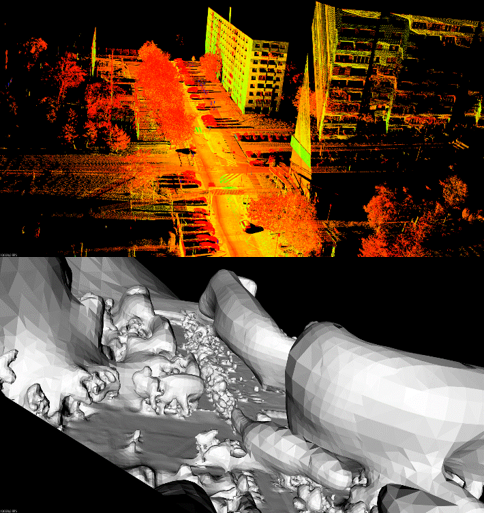
\includegraphics[width=16cm, height=13cm]{img/mesh_bad_polygons.png}
  \caption{Podvzorkované mračno bodov (hore), plocha s nadbytočnými polygónmi (dole) ($SD1$)} 
  \label{fig:mesh_bad_polygons}
\end{figure} 

\indent Po odstránení falošných polygónov, získavame očistený povrch (viď. Obr. \ref{fig:mesh_no_segmentation}). Plocha v hornej časti bola vytvorená použitím Poissonovej metódy na celé mračno bodov naraz, čo malo za následok pomerne malé rozlíšenie povrchu a stratu potrebných detailov. Tento problém bol vyriešený pomocou využitia predošlej segmentácie, čo nám umožnilo použiť rekonštrukciu na jednotlivé objekty osobitne a zabezpečilo zvýšenie zachovanej presnosti.

\begin{figure}[!htbp]
  \centering
  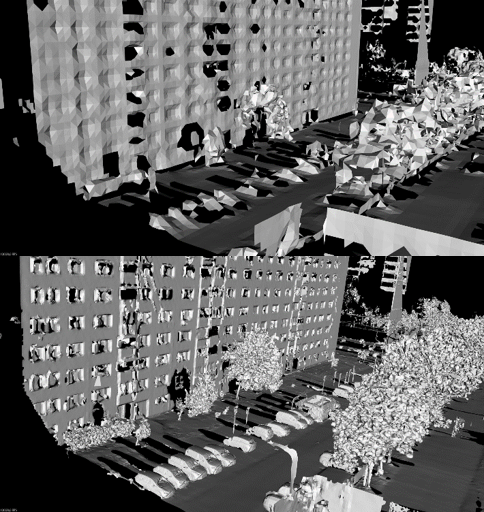
\includegraphics[width=16cm, height=13cm]{img/mesh_no_segmentation.png}
  \caption{Rekonštrukcia celého povrchu naraz (hore), rekonštrukcia individuálnych objektov (dole) ($SD1$)} 
  \label{fig:mesh_no_segmentation}
\end{figure} 

\indent Poissonová metóda je založená na správnom odhade normál, čo viedlo ku ďalšiemu problému (Obr. \ref{fig:mesh_bad_normals}). Pri odhade normál nastáva nejasnosť, či majú byť normály otočené o 180 stupňov alebo nie, pričom o tom rozhoduje umiestnenie tzv. hľadiska. Použité sady dát boli získané s pohyblivého vozidla, pričom objekty nasnímali z viacerých uhlov, čo znamená, že každý objekt má niekoľko hľadísk. Nesprávne umiestnenie hľadiska má za následok vznik trhlín, čo sa ale dá vo veľkej miere vyriešiť, pomocou umiestnenia hľadiska do ťažiska menších objektov alebo naopak ďaleko od väčších objektov.

\begin{figure}[ht]
  \centering
  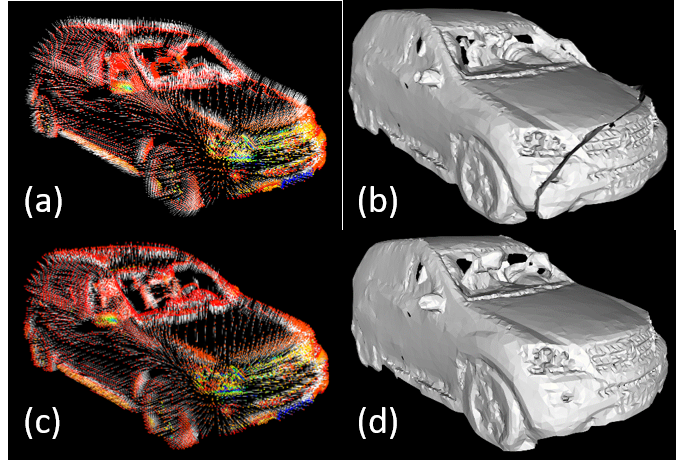
\includegraphics[width=16cm, height=10.25cm]{img/mesh_bad_normals.png}
  \caption{(a) Nesprávny odhad normál (b) Rekonštrukcia zo nesprávneho odhadu normál (c) Správny odhad normál (d) Rekonštrukcia zo správneho odhadu normál ($SD1$)} 
  \label{fig:mesh_bad_normals}
\end{figure} 

\indent Posledný problém Poissonovej metódy, bolo vytvorenie príliš veľkého počtu polygónov, aj napriek predošlému podvzorkovaniu. Tento problém sme vyriešili pridaním kvadratickej decimácie vrcholov polygónov (viď. kapitola \ref{sec:decimation}), ktorá zabezpečila zníženie pamäťovej náročnosti povrchu a súčasné zachovanie detailov (viď. Obr. \ref{fig:decimation_results}), pričom predošlé podvzorkovanie zlepšilo jeho efektivitu.

\begin{figure}[!htbp]
  \centering
  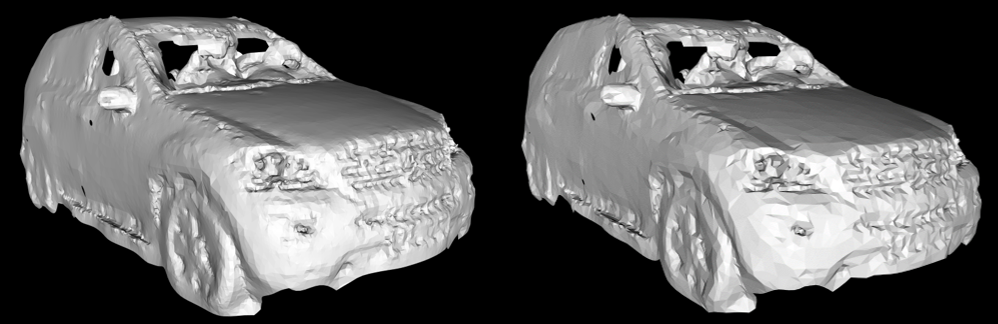
\includegraphics[width=16cm, height=5.25cm]{img/decimation_results.png}
  \caption{Porovnanie originálneho objektu (vľavo) so zdecimovaným (vpravo) pri znížení pamäťovej náročnosti o 70\%} 
  \label{fig:decimation_results}
\end{figure} 

\indent Po odstránení predošlých problémov, dosiahla rekonštrukcia vysoké zníženie pamäťovej náročnosti (viď. Tab. \ref{table:mesh_results}) a súčasné zachovania detailov. Celý postup rekonštrukcie bol vykonaný pre následujúcu konfiguráciu parametrov:

\begin{itemize}
  \setlength\itemsep{0.2em}
  \item Hĺbka oktálového stromu (objekty, zem) = 9 ; 13
  \item Hĺbka riešenia Laplcovej rovnice = 10
  \item Hĺbka extrahovaného izo povrchu = 10
  \item Počet vzoriek na uzol (pre vytvorenie ďalšej úrovne v oktálovom strome) = 2
  \item Prah vzdialenosti falošného polygónu = 0,013
  \item Redukčný faktor decimácie = 0,70-0,95
\end{itemize}

\begin{table} [!h]
  \begin{center} % Center the table
      \begin{tabular}{|c || c | c | c | c | c| c|} 
       \hline
        & \thead{Počet \\ vrcholov} &
          \thead{Počet \\ polygónov} &
          \thead{Potrebná \\ pamäť [MB]} &
          \thead{Zmenšenie potrebnej pamäti \\ oproti mračnu bodov [\%]} \\ [0.5ex]    
       \hline\hline
       \textbf{SD1} & 2 382 215  & 4 099 270 & 78,00 & 64,81 \\ 
       \hline
       \textbf{SD2} & 998 040  & 1 683 075 & 32,20 & 81,72 \\
       \hline
       \textbf{SD3} &  1 454 153  & 2 639 484 & 49,30 & 64,83 \\
       \hline
       \textbf{SD4} & 741 312  & 1 327 302 & 24,90 & 67,41 \\
       \hline
       \textbf{SD5} & 2 261 276  & 4 095 192 & 76,60 & 26,83 \\ 
       \hline
      \end{tabular}
  \caption{Výsledné hodnoty rekonštruovaných povrchov pre jednotlive súbory dát}
  \label{table:mesh_results}
  \end{center}
\end{table}

\subsection{Textúrovanie povrchu}
\noindent V poslednej časti sa zameriame na textúrovanie povrchu pomocou dát z kamery. Vytvorený povrch obohatíme o vizuálny realizmus, tak že mu pridáme informácie o farbe, drsnosti a ďalších rôznych atribútoch, pomocou čoho nadobudne hĺbku a zvýši tak predstavu o priestore.
\newline\indent Ako prvý krok textúrovania, je namapovanie jednotlivých vrcholov polygónov, na príslušné UV súradnice z kamerovej fotky. Pre tento účel potrebujeme transformovať vrcholy polygónov do súradnicového systému kamery (použitím poskytnutých transformácií), čím zabezpečíme, že kamera je v počiatku súradnicového systému a následná projekcia bude jednoduchšia. Na obrázku \ref{fig:texture_camera_image}, môžeme vidieť, že ide o 360 stupňový ekvidistantný (z ang. equirectangular) typ fotky, čo znamená, že dané vrcholy polygónov projektujeme na jednotkovú guľu, pričom ich UV súradnice sú rovné normalizovaným polárnym súradniciam gule, a teda môžeme ich získať pomocou následujúceho vzťahu:

\begin{equation}
  U = \frac{atan2\left(\dfrac{pt_y}{\sqrt{pt_x^2 + pt_y^2 + pt_z^2}} , \dfrac{pt_x}{\sqrt{pt_x^2 + pt_y^2 + pt_z^2}}\right)} {2\Pi} + 0,5
  \label{eq:texturing2}
\end{equation}
\begin{equation}
  V = \frac{asin\left(\dfrac{pt_z}{\sqrt{pt_x^2 + pt_y^2 + pt_z^2}}\right)} {2\Pi} + 0,5
  \label{eq:texturing3}
\end{equation} 
\\
\noindent kde $pt$ je vrchol polygónu a UV súradnice sú normalizované v rozsahu (0-1).
\newline\indent Keď už vieme mapovať súradnice fotky na súradnice polygónov, musíme vyriešiť, ako textúrovať povrch z viacerých fotiek. Vo väčšine prípadov, objekty bližšie ku kamere bývajú ostrejšie, zatiaľ čo vzdialenejšie objekty, začínajú byť skreslené a rozmazané. Z tohto dôvodu si pre každý polygón ukladáme informáciu o najbližšej kamere, z ktorej ho následne otextujeme, čím zabezpečíme požadovaný výsledok (Obr. \ref{fig:texture_process}a).
\newline\indent Predošlým krokom sme zabezpečili pomerne dobrý výsledok, ale takýmto spôsobom dochádza ku textúrovaniu povrchov, ktoré v skutočnosti kamera nevidí. Využijeme preto \acrshort{pcl} implementáciu sledovania lúčov (z ang. ray tracing), ktorá je založená na reprezentácií pomocou oktálového stromu. Metóda vysiela lúč z bodu kamery do jednotlivých vrcholov polygónov a zisťuje, či dochádza ku kolízií s inými polygónmi (voxelmi), ktoré ležia medzi nimi. Takto vieme zabezpečiť, aby bol texturovaný polygón skutočne viditeľný z danej kamery a predídeme tým falošnej projekcií textúry na nevidené povrchy (Obr. \ref{fig:texture_process}b).
\newline\indent Posledný problém, ktorý sme riešili, bolo odstránenie statickej prekážky. Mohli sme si všimnúť, že na použitých fotkách sa nachádza samotné auto, z ktorého boli zbierané dáta a nakoľko sa toto auto vždy nachádza najbližšie ku kamere, zanechávalo po sebe falošnú textúru na ceste. Tento problém sme vyriešili manuálnym zadefinovaním polygónu, ktorý obkresľuje okraje auta (Obr. \ref{fig:texture_camera_image}) a následnou detekciou, či daná UV koordinácia leží vo vnútri tohto polygónu, sme príslušné polygóny povrchu automaticky označili za nevidené, pričom neskôr boli otexturované z rozdielnej fotky (Obr. \ref{fig:texture_process}c).
\newline\indent Pre celý predošlý postup sme využívali \acrshort{pcl} knižnicu, ktorá do istej miery ponúkala rozhranie pre mapovanie a textúrovanie povrchu, pričom výsledky boli dosiahnuté pri následujúcej konfigurácií parametrov:

\begin{itemize}
  \setlength\itemsep{0.2em}
  \item Hĺbka oktálového stromu = 3
  \item Rozlíšenie oktálového stromu = 0,05
  \item Počet použitých fotiek = 50 (20\%)
\end{itemize}

\vfill
\begin{figure}[!htbp]
  \centering
  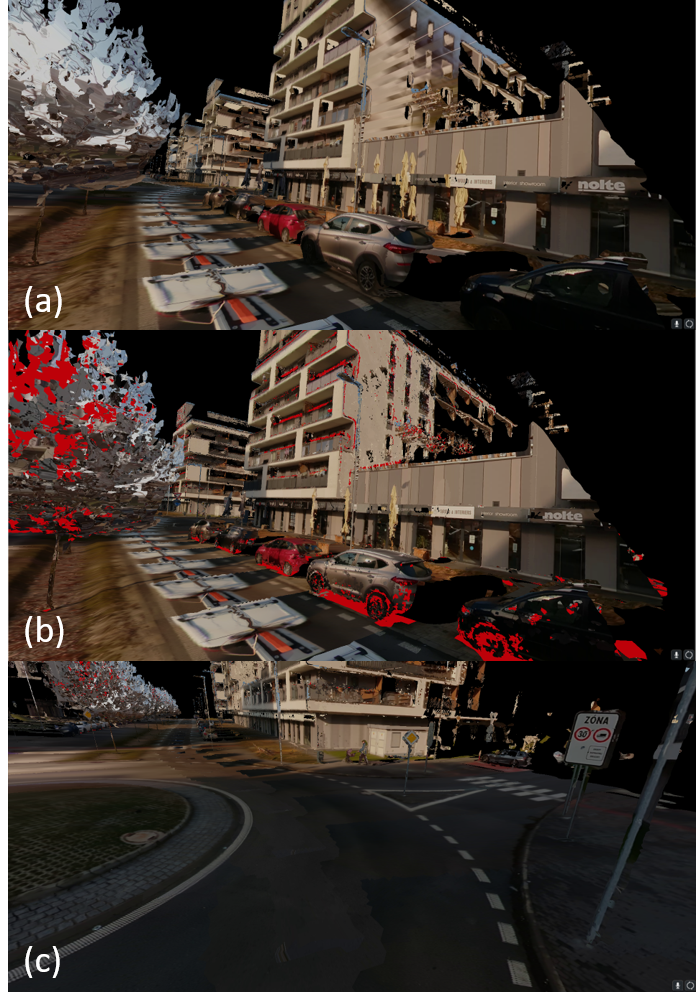
\includegraphics[width=16cm, height=20cm]{img/texturing_process.png}
  \caption{(a) Textúrovanie povrchu z najbližšej kamery (b) Textúrovanie z najbližšej kamery, iba ak kamera skutočne vidí povrch (červené polygóny nevidené žiadnou kamerou) (c) Odstránenie statickej prekážky auta na ceste ($SD2$)} 
  \label{fig:texture_process}
\end{figure}
\vfill\clearpage 

\vfill
\begin{figure}[H]
  \centering
  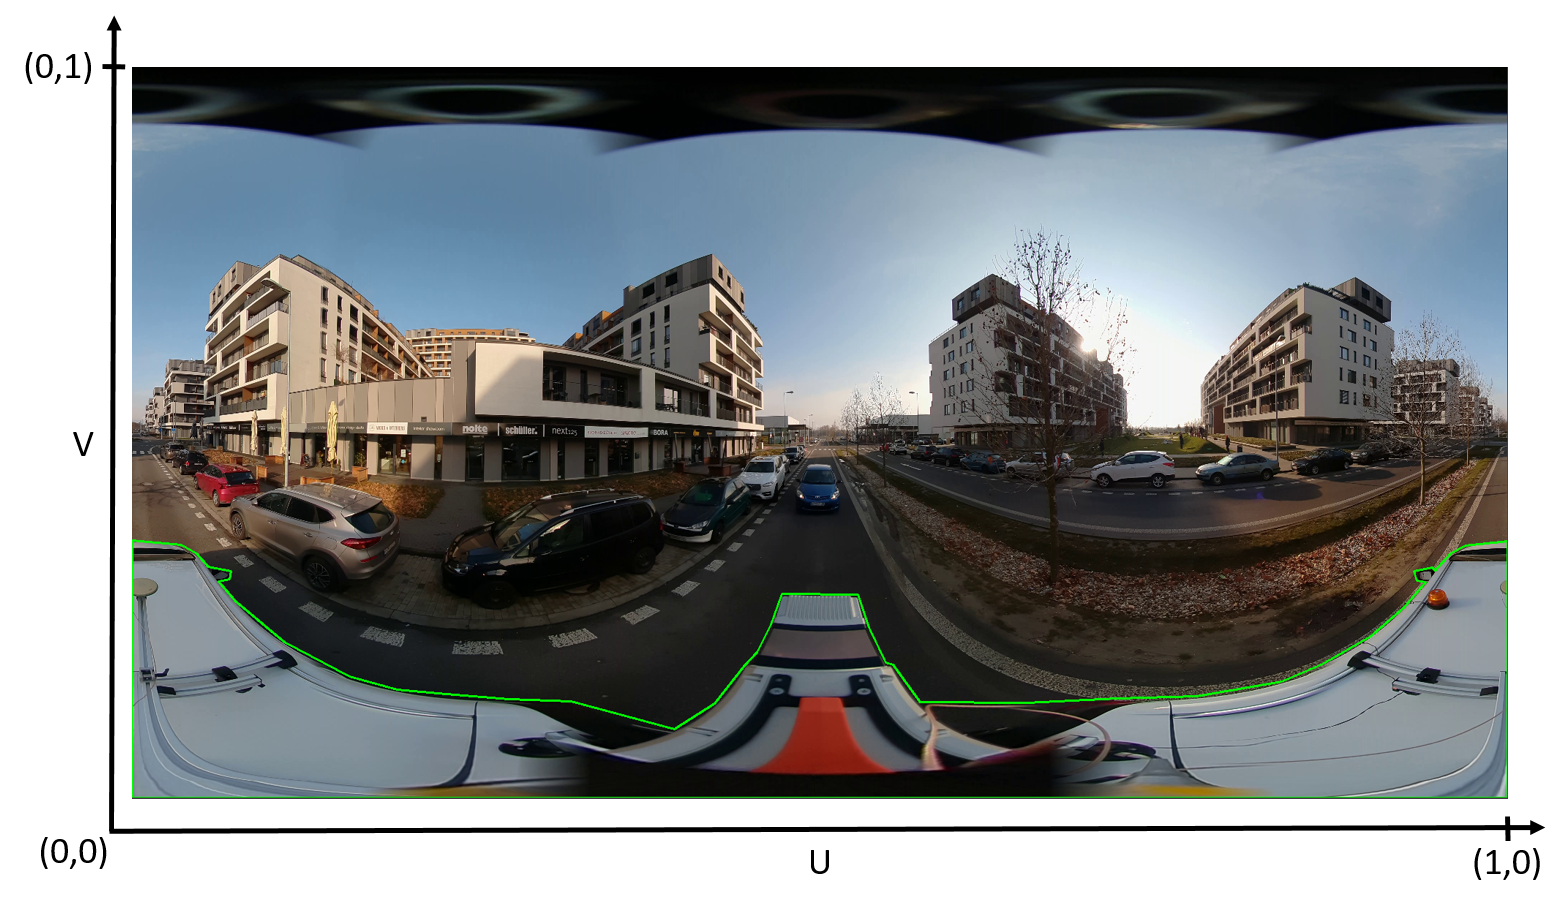
\includegraphics[width=16cm, height=10cm]{img/texture_camera_image.png}
  \caption{Ukážka kamerovej fotky s označeným autom, pomocou zeleného polygónu ($SD2$)} 
  \label{fig:texture_camera_image}
\end{figure} 
\vfill\clearpage

\section{Overenie riešenia}
\noindent V poslednej časti tejto práce overíme predošlé riešenie pomocou niekoľkých experimentov, pričom väčšina z nich bude vykonaná pomocou vizuálnej kontroly, nakoľko vo väčšine prípadov nemáme inú možnosť porovnania. Zameriame sa na jednotlivé kroky postupu, pričom ukážeme ich správnosť fungovania, vytkneme niektoré nedostatky a na záver ukážeme ich dôsledok na vytvorený povrch.

\subsection{Overenie separácia bodov zeme}
\noindent V tejto podkapitole sa zameriame na separácia bodov zeme, pričom pri tomto kroku hral dôležitú úlohu šum, a preto sa zameriame hlavne na neho. Pre tento účel sme využili sady dát $SD3$ a $SD5$, nakoľko slúžia ako validačné súbory dát a navyše boli získané pomocou rozdielneho \acrshort{lidar}-u, ktorý obsahuje vyššiu úroveň zle nasnímaných bodov, v podobe šumu.
\newline\indent Nedostatky progresívneho morfologického filtra môžeme vidieť v prípade, kedy auto nasnímalo falošné body na trase ktorou prešlo (Obr. \ref{fig:Parking_ground} a  \ref{fig:Parking_ground_detail}). Môžme si všimnúť, že body boli husto zoskupené, a tým pádom neboli odstránené pomocou filtrovania odľahlých bodov, čo zapríčinilo nesprávnosť fungovania filtra v tejto oblasti. S princípu fungovania progresívneho morfologického filtra vychádza, že v danom ``okne''  vyhodnotí najnižšie body, ako body zeme, čo v tomto prípade spôsobilo, že falošné body boli vyhodnotené ako body zeme, namiesto skutočných nad nimi.

\begin{figure}[!htbp]
  \centering
  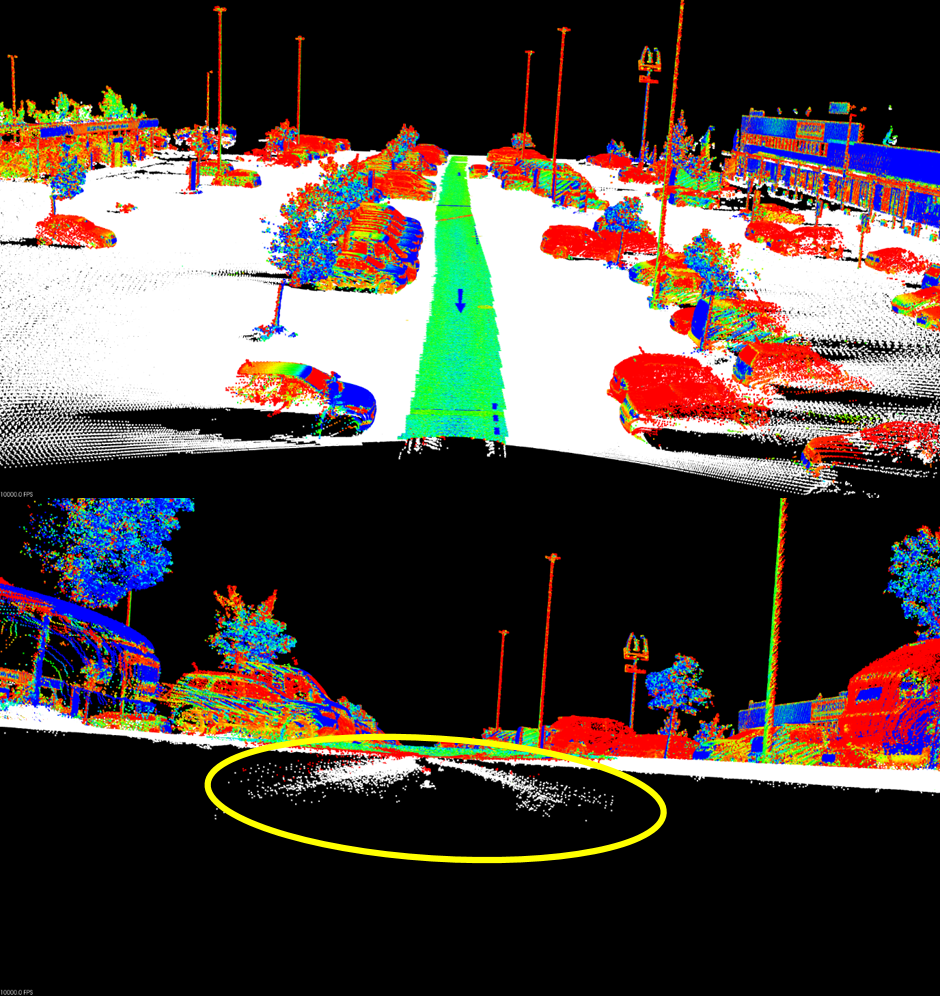
\includegraphics[width=16cm, height=8.5cm]{img/Parking_ground.png}
  \caption{Body cesty klasifikované ako body objektov ($SD3$)} 
  \label{fig:Parking_ground}
\end{figure}

\begin{figure}[!htbp]
  \centering
  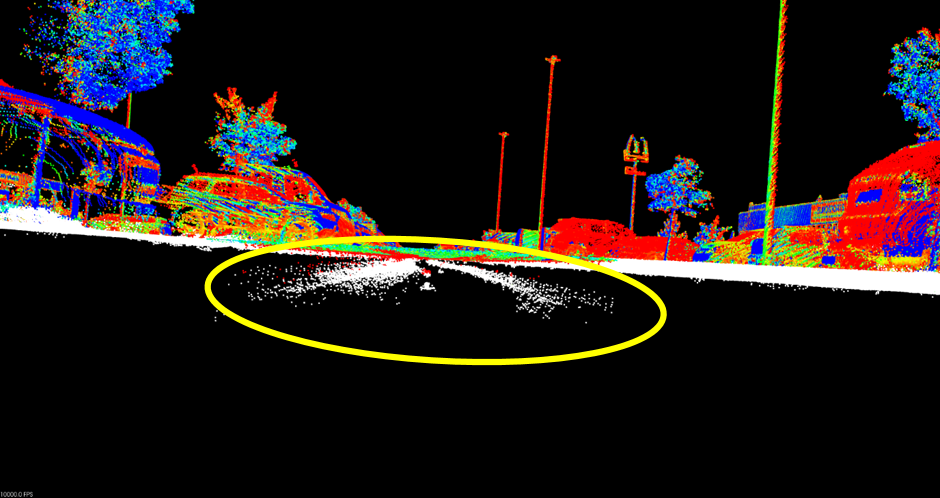
\includegraphics[width=16cm, height=9cm]{img/Parking_ground_detail.png}
  \caption{Body cesty klasifikované ako body objektov (detail šumu) ($SD3$)} 
  \label{fig:Parking_ground_detail}
\end{figure}

\indent Následok šumu bolo ešte lepšie vidieť v prípade, kedy boli dáta získané z letiaceho dronu (Obr. \ref{fig:UAV_ground}), kde miera šumu bola omnoho väčšia a postihovala takmer celé mračno bodov. V tomto prípade dochádzalo ku nesprávnej filtrácií nie len pri bodoch zeme, ale navyše aj pri bodoch striech, ktoré boli nesprávne označené za body zeme. Tento výsledok bol zapríčinení šumom a taktiež nízkym nastavením maximálnej veľkosti ``okna'' pre tento súbor dát. Môžme teda vidieť, že v prípade vysokej úrovne šumu filter vo veľkej miere zlyháva, čo bude mať za následok nižšiu úroveň podvzorkovania. 

\newpage\vfill
\begin{figure}[!htbp]
  \centering
  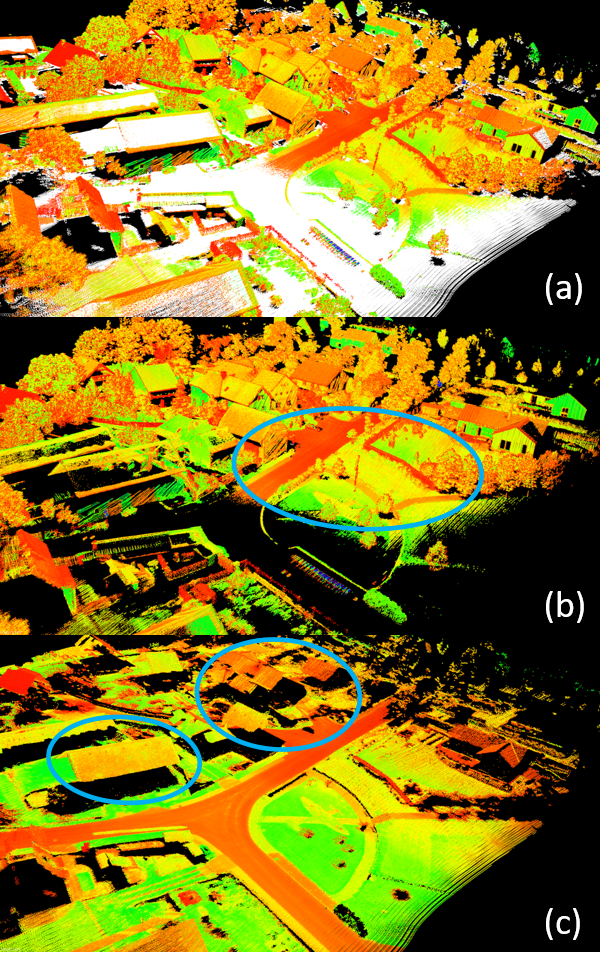
\includegraphics[width=16cm, height=21cm]{img/UAV_ground.png}
  \caption{Odolnosť morfologickej separácie bodov zeme na šum - (a) Mračno bodov objektov (pôvodná farba), body zeme (biela farba) (b) Body objektov obsahujú aj body zeme (c) Body zeme obsahujú strechy budov ($SD5$)} 
  \label{fig:UAV_ground}
\end{figure}
\vfill\clearpage 

\indent Medzi posledné nedostatky filtrovania zeme patrilo to, že progresívny morfologický filter berie za body zeme, aj body tesne nad jeho skutočným povrchom (Obr. \ref{fig:seprartion_wheels}) a taktiež má problém s málo hustými bodmi, ktoré sú v blízkej tesnosti zeme (Obr. \ref{fig:seprartion_density}).

\vfill
\begin{figure}[!htbp]
  \centering
  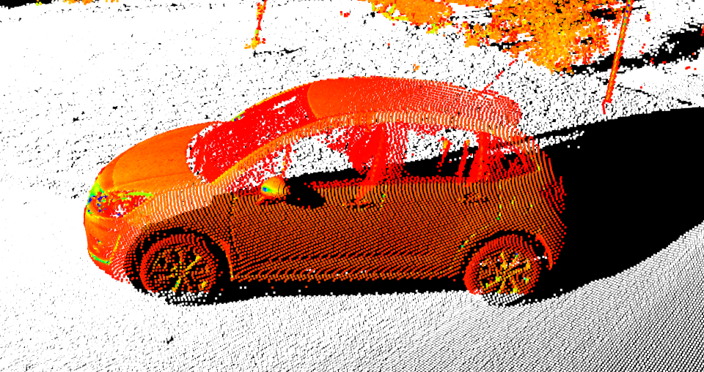
\includegraphics[width=16cm, height=8.5cm]{img/seprartion_wheels.png}
  \caption{Body kolies auta vyhodnotená ako body zeme ($SD1$)} 
  \label{fig:seprartion_wheels}
\end{figure}

\begin{figure}[!htbp]
  \centering
  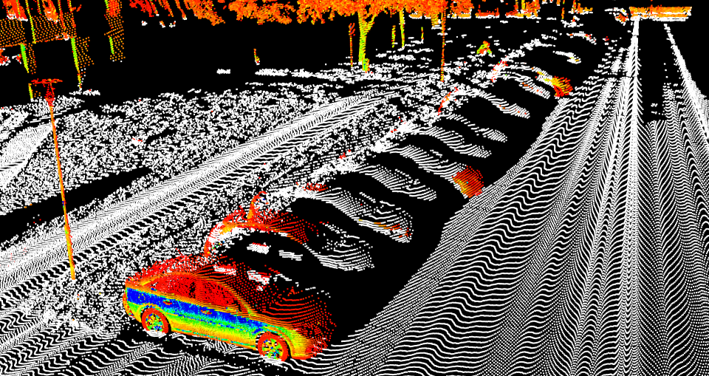
\includegraphics[width=16cm, height=8.5cm]{img/seprartion_density.png}
  \caption{Málo hustne body áut vyhodnotené ako body zeme ($SD1$)} 
  \label{fig:seprartion_density}
\end{figure}

\subsection{Overenie generovania supervoxelov a segmentácie}
\noindent V tejto podkapitole sa zameriame na overenie zhlukovania bodov do supervoxelov a spojíme to so segmentáciou, nakoľko tieto kroky spolu blízko súvisia. Vizuálne overíme jednotlivé kroky, pričom si ukážeme ich nedostatky.
\newline\indent Zhlukovanie bodov do supervoxelov bolo z veľkej časti úspešné, ale vznikol problém v prípade, kedy sa pri sebe v malej vzdialenosti nachádzalo viacero objektov. V takomto prípade niekedy supervoxely prechádzali cez hranice objektov, čo bolo obzvlášť pravdou v prípade ak sa jednalo o vegetáciu (Obr. \ref{fig:supervoxel_connecting}).

\begin{figure}[!htbp]
  \centering
  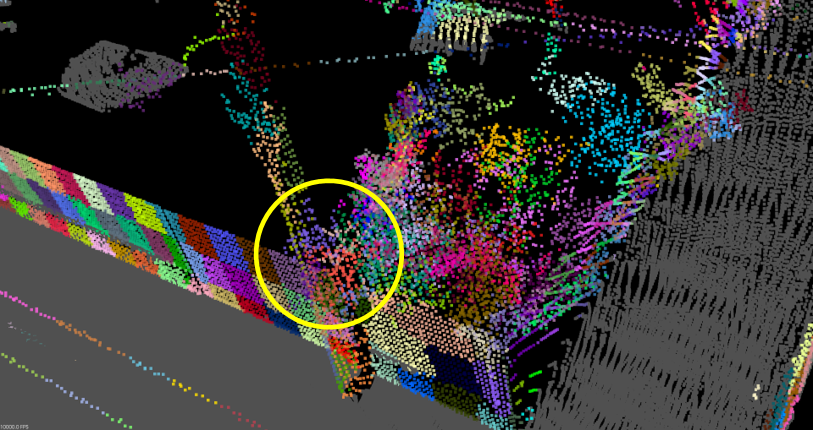
\includegraphics[width=16cm, height=9cm]{img/supervoxel_connecting.png}
  \caption{Prechod supervoxelov medzi bodmi stĺpu a bodmi stromu ($SD4$)} 
  \label{fig:supervoxel_connecting}
\end{figure} 

\indent V prípade samotnej segmentácie sme sa stretli s podobným problémom, a teda ak bolo pri sebe viacero objektov v malej vzdialenosti, tak v niektorých prípadoch nastalo ich spojenie (Obr. \ref{fig:segmentation_connecting}), čo čiastočne súviselo s predošlou chybou pri vytváraní supervoxelov. Navyše v prípade veľkých, ale aj menších horšie nasnímaných objektov dochádzalo ku rozdeleniu objektu na viacero menších objektov (Obr. \ref{fig:segmentation_big} a \ref{fig:segmentation_devide}), čo ale v niektorých prípadoch nemuselo byť nevyhnutnou chybou. 

\begin{figure}[!htbp]
  \centering
  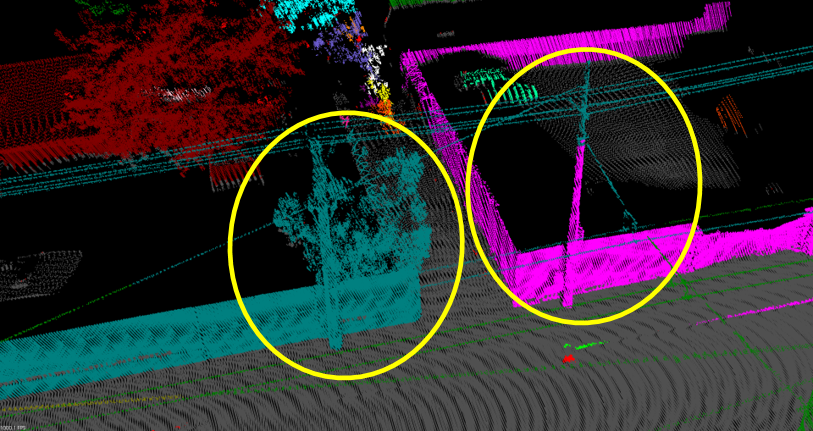
\includegraphics[width=16cm, height=9cm]{img/segmentation_connecting.png}
  \caption{Body viacerých objektov segmentované ako jeden objekt ($SD4$)} 
  \label{fig:segmentation_connecting}
\end{figure} 

\begin{figure}[htbp]
  \centering
  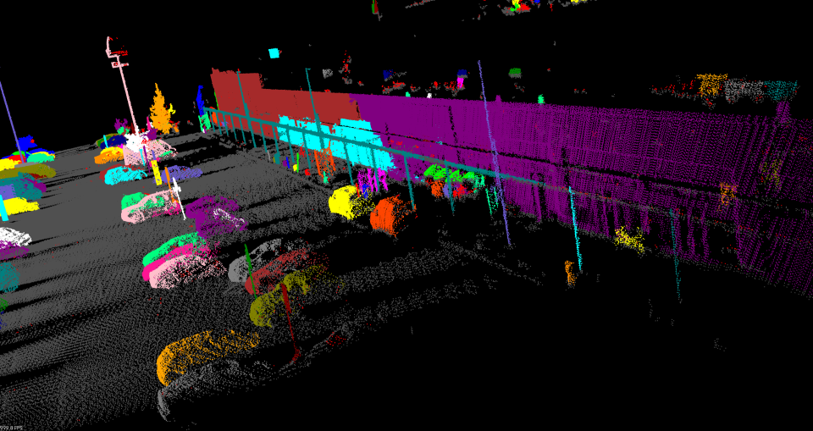
\includegraphics[width=16cm, height=9cm]{img/segmentation_big.png}
  \caption{Segmentovanie bodov veľkej budovy na viacero objektov ($SD3$)} 
  \label{fig:segmentation_big}
\end{figure} 

\begin{figure}[!htbp]
  \centering
  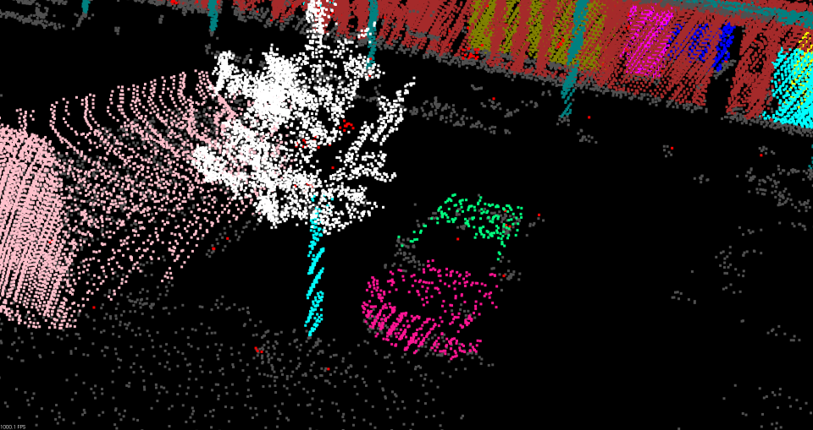
\includegraphics[width=16cm, height=9cm]{img/segmentation_devide.png}
  \caption{Segmentovanie bodov stromu a auta na viacero objektov ($SD3$)} 
  \label{fig:segmentation_devide}
\end{figure} 

\newpage\vfill
\subsection{Overenie adaptívneho podvzorkovania}
\noindent Pri adaptívnom podvzorkovaní sa zameriame hlavne na vizuálne porovnanie vytvorených povrchov pre nepodvzorkované, adaptívne podvzorkované a rovnomerne podvzorkované mračná bodov, keďže dosiahnuté úrovne podvzorkovania boli ukázané skôr (Tab. \ref{table:subsampling}). Týmto porovnaním si ukážeme výhody adaptívneho prístupu oproti bežnému a zároveň si ukážeme niektoré nedostatky.
\newline\indent Dosiahnuté výsledky adaptívneho podvzorkovania môžeme dobre vidieť na obrázku \ref{fig:adaptive_comparison}, kde pre porovnanie bolo pridané rovnomerné podvzorkovanie pomocou voxelovej mriežky (neadaptívne), ktoré bolo nastavené, tak aby dosahovalo takmer rovnakú úroveň podvzorkovania (počtu bodov). Z vizuálneho hľadiska si môžeme všimnúť, že boli zachované ostrejšie detaily najmä v oblasti značky auta, pričom pri neadaptívnom prístupe, začali miznúť. Adaptívne podvzorkovanie znížilo výpočtovú náročnosť pri rekonštrukcií povrchu a zároveň pri porovnaní s nepodvzorkovaným mračnom bodov, zachovalo potrebné črty objektu.
\newline\indent Pre ďalšie porovnanie sme využili menej husté mračno bodov z rozdielneho súboru dát (Obr. \ref{fig:adaptive_comparison2}). V tomto prípade z vizuálneho hľadiska nie je vidieť výrazný rozdiel, čo bolo najmä zapríčinené menšou hustotou bodov (nižšou prítomnosťou detailov). Ďalej si môžme všimnúť, že v tomto prípade pomáha adaptívne podvzorkovanie vyhladeniu rovnejších povrchov (kapota auta), ale na druhú stranu zlyháva pri efektívnom znížení počtu bodov na zašumenom povrchu (čelné sklo).

\newpage\vfill
\begin{figure}[!htbp]
  \centering
  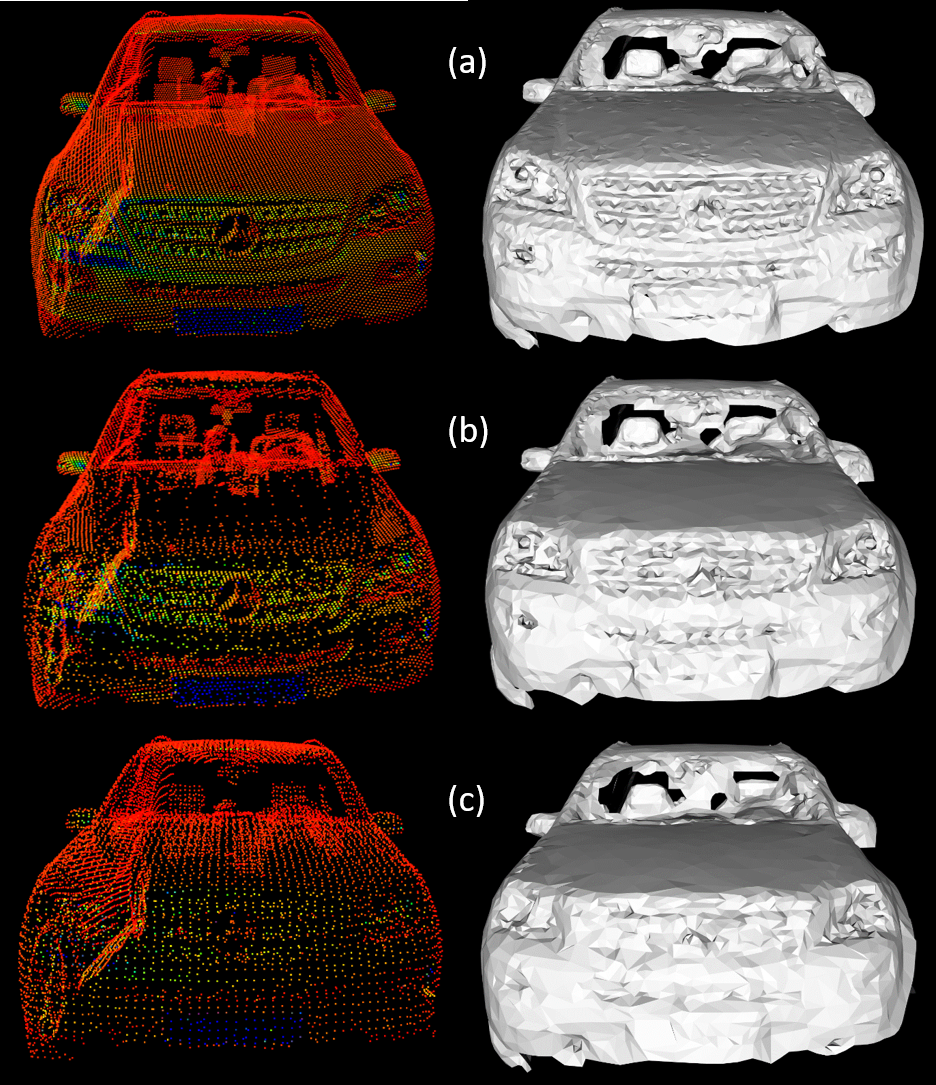
\includegraphics[width=16cm, height=21cm]{img/adaptive_comparison.png}
  \caption{Mračná bodov a ich príslušný povrch - (a) Nepodvzorkované mračno bodov (b) Adaptívne podvzrokované mračno bodov (c) Rovnomerne podvzorkované mračno bodov pomocou voxelovej mriežky ($SD1$)} 
  \label{fig:adaptive_comparison}
\end{figure}
\vfill\clearpage 

\newpage\vfill
\begin{figure}[!htbp]
  \centering
  \includegraphics[width=16cm, height=21cm]{img/adaptive_comparison2.png}
  \caption{Mračná bodov a ich príslušný povrch - (a) Nepodvzorkované mračno bodov (b) Adaptívne podvzrokované mračno bodov (c) Rovnomerne podvzorkované mračno bodov pomocou voxelovej mriežky ($SD3$)} 
  \label{fig:adaptive_comparison2}
\end{figure}
\vfill\clearpage 

\subsection{Overenie rekonštrukcie povrchu}
\noindent Pri rekonštrukcií povrchu sme dosiahli pomerne vysoké zníženie pamäťovej náročnosti oproti pôvodnému mračnu bodov (viď. Tab. \ref{table:mesh_results}). V tejto podkapitole sa preto budeme zaoberať vizuálnou kontrolou dosiahnutých výsledkov, pričom sa zameriame aj na nedostatky spôsobené predošlými krokmi.
\newline\indent Ako prvé sme overili rekonštrukciu povrchu v prítomnosti falošných bodov v podobe šumu (Obr. \ref{fig:noise_mesh} a \ref{fig:ground_separation_mesh}). V prvom prípade bola úroveň šumu príliš vysoká, na základe čoho zlyhala predošlá separácia bodov, adaptívne podvzorkovanie vyhodnotilo šum za dôležité body a viedlo to ku vzniku drsného povrchu, ktorý nie je prirodzený. V ďalšom prípade taktiež čiastočne zlyhala separácia bodov zeme, ale vďaka nižšej úrovni šumu, bol tento nedostatok zakrytý zemou (v podobe objektu), ktorá sa pomerne plynulo spojila so skutočnou zemou. Nevýhodou zlyhania predošlých krokov je nižšia úroveň podvzorkovania a vytvorenie väčšieho počtu polygónov, ktoré navyše opisujú falošné dáta.

\begin{figure}[!htbp]
  \centering
  \includegraphics[width=16cm, height=9cm]{img/noise_mesh.png}
  \caption{Vznik drsného povrchu pri nesprávnej separácií bodov zeme (Obr. \ref{fig:UAV_ground}) a rekonštrukcií zo zašumených dát ($SD5$)} 
  \label{fig:noise_mesh}
\end{figure} 

\newpage\vfill
\begin{figure}[!htbp]
  \centering
  \includegraphics[width=16cm, height=8.5cm]{img/ground_separation_mesh.png}
  \caption{Hladký prechod medzi viacerými povrchmi zeme, aj napriek nesprávnej separácií zeme (Obr. \ref{fig:Parking_ground}) ($SD3$)} 
  \label{fig:ground_separation_mesh}
\end{figure} 

\indent Ďalším nedostatkom pri rekonštrukcií boli prípady, kedy zlyhala segmentácia, čo zapríčinilo spojenie povrchu viacerých objektov (Obr. \ref{fig:connecting_mesh}) a odstránenie skutočnej medzery medzi nimi. Taktiež sa našli prípady, kedy aj napriek úpravám zlyhal odhad normál, čo zapríčinilo vytvorenie trhlín v povrchu (Obr. \ref{fig:normal_mesh}).

\vfill
\begin{figure}[!htbp]
  \centering
  \includegraphics[width=16cm, height=8.5cm]{img/connecting_mesh.png}
  \caption{Prepojenie viacerých objektov spolu, na základe zlej segmentácie (Obr. \ref{fig:segmentation_connecting}) ($SD4$)} 
  \label{fig:connecting_mesh}
\end{figure} 

\begin{figure}[!htbp]
  \centering
  \includegraphics[width=16cm, height=8.5cm]{img/normal_mesh.png}
  \caption{Výskyt trhlín na základe zlého odhadu normál ($SD3$)} 
  \label{fig:normal_mesh}
\end{figure} 

\indent V poslednom rade sme sa zamerali na dôveryhodnosť povrchu, kde sme si všimli, že rekonštrukcia má problém s úzkymi objektami a vegetáciou (Obr. \ref{fig:cable_mesh} a \ref{fig:tree_mesh}), pričom tento efekt bol posilnený neúplným odstránením nadbytočných polygónov na hranách objektu.

\vfill
\begin{figure}[!htbp]
  \centering
  \includegraphics[width=16cm, height=8.5cm]{img/cable_mesh.png}
  \caption{Problém Poissonovej rekonštrukčnej metódy s rekonštrukciou úzkych objektov (trolejbusové vedenie) ($SD4$)} 
  \label{fig:cable_mesh}
\end{figure} 

\begin{figure}[!htbp]
  \centering
  \includegraphics[width=16cm, height=9cm]{img/tree_mesh.png}
  \caption{Problém Poissonovej rekonštrukčnej metódy s dôveryhodnou rekonštrukciou stromov  ($SD1$)} 
  \label{fig:tree_mesh}
\end{figure} 

\subsection{Overenie textúrovania povrchu}
\noindent Textúrovanie povrchu dosiahlo pomerne dobré výsledky a obohatilo to povrch o dávku realizmu, avšak nachádzali sa tam nedostatky, ku ktorým sa teraz vyjadríme. 
\newline\indent Ako prvý problém sa prejavilo využitie sledovania lúčov, ktoré bolo založené na využití oktálového stromu. Vo veľkej miere to síce odstránilo falošné textúrovanie, ale kvôli neúplnému zachyteniu geometrie polygónov pomocou voxelov, dochádzalo ku mozaikovému textúrovaniu a taktiež niektoré polygóny neboli otextúrované vôbec, aj napriek tomu, že boli v skutočnosti videné (Obr. \ref{fig:texturing_problems}a).
\newline\indent Ďalší nedostatok vznikol pri textúrovaní s viacerých fotiek. Na hranách medzi jednotlivými snímkami dochádzalo ku ostrému prechodu farby (Obr. \ref{fig:texturing_problems}b), čo vytváralo neprirodzený vzhľad. Tento problém by sa dal adresovať, pomocou využitia Gaussového filtra na jednotlivých hranách, pre zjemnenie ich prechodu.
\newline\indent Posledný nedostatok sa týkal dynamických objektov, ktoré boli pri získavaní mračna bodov odstránené, ale ostali na fotkách z kamery. Tieto objekty spôsobujú falošné textúrovanie iných objektov (Obr. \ref{fig:texturing_problems}c) a pre ich odstránenie by bolo potrebné implementovať detekciu dynamických objektov na fotkách. 

\begin{figure}[!htbp]
  \centering
  \includegraphics[width=16cm, height=20cm]{img/texturing_problems.png}
  \caption{(a) Mozaikové textúrovanie kvôli zlej reprezentácií polygónov pomocou oktálového stromu (sledovanie lúčov) (b) Ostrý prechod farby medzi viacerými snímkami (c) Neodstránenie dynamických objektov (auto na ceste) ($SD2$)} 
  \label{fig:texturing_problems}
\end{figure}
\vfill\clearpage  